% filepath: /gpfs/mcc/HT04543/jxc06/jxc74-jxc06/projects/FusionComputingLab/PhaseV_FCL1/codes/U-Net-LES/Paper_Germano_GenerativeAI.tex
\documentclass[authoryear,preprint,review,12pt]{elsarticle}

\usepackage[a4paper,margin=2cm]{geometry}
\usepackage{amsmath,amssymb}
\usepackage{graphicx}
\usepackage{hyperref}
\usepackage{booktabs}
\usepackage{subcaption}
\usepackage{algorithm}
\usepackage{algorithmic}
\usepackage{todonotes}

\hypersetup{colorlinks=true,linkcolor=black,citecolor=black,urlcolor=cyan}

\journal{Computer Physics Communications}

\begin{document}

\begin{frontmatter}

\title{
    % Learning Germano Differential-filtered DNS fields via Generative AI to accelerate edge plasma turbulence simulations
    Learning differential filter inversion with deep learning for modelling subgrid turbulence in edge plasmas
}

\author{Jony Castagna}
\author{Josh Williams}

\affiliation{
  organization={UKRI-STFC Hartree Centre},
  addressline={Daresbury Laboratory},
  city={Warrington},
  postcode={WA4 4AD},
  country={United Kingdom}
}

\begin{abstract}
We present a novel method which combines the invertibility of Germano's filter with generative artificial intelligence to accelerate edge plasma turbulence simulations.
Rather than learning the mapping from coarse LES fields to fine DNS, the proposed method learns the mapping from coarse LES fields to Germano Differential-filtered DNS fields. 
We then use the inverse of Germano's filter to reconstruct the fine-scale DNS fields and hence calculate exactly the nonlinear terms in the governing equations, or the subgrid-scale terms in the LES.

The method is tested on the Hasegawa--Wakatani and modified Hasegawa--Wakatani plasma turbulence models at $256^2$ and $512^2$ DNS resolutions using 2, 4 and 8 times smaller LES grids in each direction. We compare the generative model with DNS and conventional LES diagnostics, including energy, enstrophy, spectra, probability distributions, poloidal and radial fluxes and computational cost. Validation extends to 1000 simulation time units for HW and 100 for mHW, whose faster dynamics lead toward laminarization. Finer LES meshes retain several integral and spectral features, while the coarsest HW $256^2$ reconstruction shows substantial energy, enstrophy and transport deficits and its mHW counterpart develops excess fluctuations and transport. Thousand-time-unit HW and mHW benchmarks show MPI task-time reductions of 4.82--49.45, with a maximum wall-clock speedup of 1.55.
\end{abstract}

\begin{keyword}
Large Eddy Simulation \sep Generative artificial intelligence \sep 
Hasegawa--Wakatani model \sep plasma turbulence \sep deconvolution methods
\end{keyword}

\end{frontmatter}
%----------------------------------------------------------------
%
%
%
%
%
%
%
%----------------------------------------------------------------
\section{Introduction}\label{sec:Introduction}
The dynamics of plasma turbulence in the edge region of nuclear fusion reactors are best studied through direct numerical simulation (DNS). This approach is highly prohibitive, and restricts simulations to small systems far below the resolution required for future tokamaks such as ITER, even on modern exascale hardware. Alternatively, simpler models are used in 1D or 2D with diffusion profiles taken from experiments.
One faster alternative for studying edge plasmas without resolving all scales of the turbulence is using Large Eddy Simulations (LES) on coarse grids. 
However, but an ad-hoc modelling of the sub-grid scales is required. In strongly magnetized plasma it is notoriously very challenging to find correct models \citep{leddy2016thesis}, as the energy injected at small length and, via inverse cascade, propagated to large scales, as described on the work on 2D turbulence by \citet{kraichnan_inertial_1967}.

One standard problem studied in plasma edge turbulence is the 2D Hasegawa--Wakatani (HW) model \citep{hasegawa_self-organization_1987}, which couples plasma-density and electrostatic-potential fluctuations to describe resistive drift-wave turbulence. To account for zonal-flow dynamics, the modified Hasegawa--Wakatani (mHW) model excludes the zonal components from the resistive coupling \citep{numata_bifurcation_2007}. This reflects the absence of a parallel-electron response for zonal modes, which are constant on a flux surface. Removing their direct resistive damping allows zonal shear flows to develop and, depending on the parameters, suppress drift-wave turbulence. 
Turbulence modelling of the HW system through models such as Smagorinsky has been studied by \citet{leddy2016thesis}. Recently, fully data-driven models of this problem have also been studied \citep{gahr2024scientific, artigues2025accelerating, greif2023physics}.
The HW and mHW models provide complementary tests of an LES closure in regimes with different interactions between turbulent fluctuations and zonal flows.

Deconvolution operators for LES have been proposed in the past as Approximate Deconvolution Methods (ADM) by \citet{stolz_approximate_1999}. ADM reconstructs unfiltered flow variables based on the filtered variables, but this fails in capturing small turbulent details not present in the original simulation \todo{REF}.
However, recent interest in deep neural networks for computational fluid dynamics \citep{wang_recent_2024} has presented approaches for generating subgrid flow structures through (i) generative adversarial networks (GANs) \citep{goodfellow_generative_2014,bode_using_2021,nista2024influence,castagna_stylegan_2024}, (ii) diffusion models \citep{ho_denoising_2020,sardar2024spectrally,shu2023physicsDM} and other methods \citep{kim_unsupervised_2021, ling2016reynolds}. Each of these methodologies has pros and cons, mainly on training robustness, accuracy and speed. In our previous work \citep{castagna_stylegan_2024} we used StyleGAN \citep{karras_style-based_2019}, a model developed by NVIDIA for face synthesis, as a deconvolution operator for 2D turbulent flows. The algorithm used, named Style Eddy Simulation (StylES), showed a factor $10\times$ speedup vs single core DNS for $1024^2$ resolution. GANs such as StyleGAN often suffer from the need for a large quantity of training data to achieve stable training. Even then, reconstructing DNS fields from LES on very coarse meshes remains challenging. This is particularly true for lossy filters such as Gaussian or top-hat kernels. One class of filters for LES proposed by \citet{germano_differential_1986} are known as differential filters which are invertible at a fixed resolution. This corresponds to inverting the Helmholtz equation of a filtered variable, and has been used in particle-laden flows to reconstruct the unfiltered fluid velocity in particle drag calculations \citep{park2017particle}.
A key limitation is that typically the LES variable will be solved on a coarse grid, and the loss of information will make this no longer invertible.

In the present paper we improved our previous work on StylES \citep{castagna_stylegan_2024}, replacing the full StyleGAN architecture with a simpler U-Net based architecture, but moving the training target from the fully developed DNS fields to the Germano's filtered DNS fields (at the DNS resolution). 
The idea is that the super-resolution task is split into two parts: (i) de-aliasing the LES field by mapping from a coarse grid LES to a fine grid filtered DNS, and (ii) reconstruction the DNS from the filtered DNS on the same grid using the inverse of Germano's differential filter.
This approach allows for: a) a much faster super-resolution and hence time integration and b) simplify drastically the training process, notoriously difficult for GANs.

The paper continues as follows: Sections~\ref{sec:PhysicalModel} introduce the physical model and the LES filtering approach. Section~\ref{sec:NumericalImplementation} section explains the U-Net based architecture and the modifications needed to have a stable time integration. Moreover, details on the training and reconstruction methodology are provided. Section~\ref{sec:Results} presents the results and discussion on the performance. Finally, Section~\ref{sec:Conclusions} summarizes the findings and proposes future work, which will be mainly moving towards a full 3D implementation of the proposed methodology.

The code used to generate the results is available on the U-Net-LES repositories at \url{https://github.com/stfc/U-Net-LES} and the model weights are available on Zenodo at \url{https://doi.org/10.5281/zenodo.22973917}.
%----------------------------------------------------------------
%
%
%
%
%
%
%
%----------------------------------------------------------------
\section{Physical model}\label{sec:PhysicalModel}

\subsection{Hasegawa-Wakatani model}
In a tokamak device, one of the first simplified model which describes the transport of turbulence in the scrape-off layer is described by Hasegawa-Wakatani (HW) equations \citep{hasegawa_self-organization_1987}. This consists of a perpendicular slab to the toroidal magnetic field, with radial coordinate $x$ and poloidal coordinate $y$. The time evolution of the normalized density perturbation $n$, electrostatic potential $\phi$ and vorticity $\zeta$ are given by the two phase fluid magnetohydrodynamic equations:
\begin{align}
    \frac{\partial\zeta}{\partial t}+\{\phi,\zeta\}
    &=\alpha(\phi-n)-D_\zeta\nabla_\perp^4\zeta,
    \label{eq:hw_vorticity}\\
    \frac{\partial n}{\partial t}+\{\phi,n\}
    &=\alpha(\phi-n)-\kappa\frac{\partial\phi}{\partial y}
      -D_n\nabla_\perp^4 n.
    \label{eq:hw_density}
\end{align}
The potential follows from:
\begin{equation}
    \nabla_\perp^2\phi=\zeta,
\end{equation}
and the Poisson bracket describing the $\mathbf{E}\times\mathbf{B}$ advection is
\begin{equation}
    \{a,b\}=\partial_xa\,\partial_yb-\partial_ya\,\partial_xb.
    \label{eq:hw_poisson}
\end{equation}
The constant $\alpha$ represents the conductivity, while $\kappa=-\partial_x\ln n_0$ specifies the background density-gradient drive. Fourth-order dissipation (known as hyperviscosity) removes small-scale fluctuations. The hyperviscosity term can be rewritten in different forms, according to the numerical scheme used and the wavenumber cut-off.

For $\alpha=0$, vorticity evolves independently and the incompressible hydrodynamic equations are recovered. For large $\alpha$, the standard HW model approaches $n=\phi$. Neglecting dissipation, subtraction of the density equation gives the Hasegawa--Mima limit:
\begin{equation}
    q=\nabla_\perp^2\phi-\phi,
    \qquad
    \partial_tq+\{\phi,q\}=\kappa\partial_y\phi.
    \label{eq:hm_limit}
\end{equation}

The modified HW model removes zonal components from the coupling \citep{numata_bifurcation_2007}.
By setting:
\begin{equation}
    \langle f\rangle_y=\frac{1}{L_y}\int_0^{L_y}f(x,y,t)\,dy,
    \qquad f'=f-\langle f\rangle_y.
    \label{eq:zonal_decomposition}
\end{equation}
the equations become:
\begin{align}
    \frac{\partial\zeta}{\partial t}+\{\phi,\zeta\}
    &=\alpha(\phi'-n')-D_\zeta\nabla_\perp^4\zeta,
    \label{eq:mhw_vorticity}\\
    \frac{\partial n}{\partial t}+\{\phi,n\}
    &=\alpha(\phi'-n')-\kappa\frac{\partial\phi}{\partial y}
      -D_n\nabla_\perp^4 n.
    \label{eq:mhw_density}
\end{align}
which introduces zonal modes without parallel-electron response which. Excluding their direct resistive damping permits zonal shear flows that can suppress turbulence \citep{numata_bifurcation_2007}.

We use primes for non-zonal fluctuations and reserve tildes for LES-filtered fields. This distinction matters because the zonal average and the LES filter serve different purposes: the former defines the physical coupling, while the latter introduces the unresolved nonlinear terms discussed below.

Both HW and mHW systems are considered fully periodic in $x$ and $y$, with domain size $L_x=L_y=50.176$. The background density gradient is adjusted according to the test case, $\kappa=0.5 - 1$, as well as the dissipation coefficients are set to $D_\zeta=D_n=10^{-3} - 10^{-4}$. The parallel-electron response is $\alpha=0.5 - 1$, which are ideal values for the weakly collisional regime. 
The initial conditions are Gaussian random fields with zero mean and unit variance, filtered to remove high wavenumbers. 
The simulations are run up to 2000 time units ($t_{HW}=\Omega_{ci}t_{physical}$, where $\Omega_{ci}=\frac{ZeB}{m_i}$ is the ion cyclotron frequency). Snapshots are saved every $t_{HW}$.

\subsection{LES formulation with differential filtering}
\label{sec:GermanoDifferentialFilter}

\citet{germano_differential_1986} introduced spatial filters whose inverse is a differential operator. For the isotropic case, define:
\begin{equation}
    \mathcal{H}_\ell=I-\ell^2\nabla_\perp^2,
    \qquad \mathcal{F}_\ell=\mathcal{H}_\ell^{-1},
    \qquad \widetilde f=\mathcal{F}_\ell f.
    \label{eq:germano_filter}
\end{equation}
Thus filtering amounts to solving a Helmholtz problem, whereas its formal inverse is locally defined as:
\begin{equation}
    (I-\ell^2\nabla_\perp^2)\widetilde f=f,
    \qquad f=\widetilde f-\ell^2\nabla_\perp^2\widetilde f.
    \label{eq:germano_inverse}
\end{equation}
Here $\ell$ (usually indicated with $\alpha$ or $a$ elsewhere), is the filter width in physical space. The inverse requires boundary conditions consistent with the forward filter, where our implementation uses periodic Fourier transforms.

In Germano's unbounded three-dimensional construction, the corresponding normalized convolution kernel is $G_\ell(r)=\exp(-r/\ell)/(4\pi\ell^2r)$. For our two-dimensional periodic domain, the filter is instead specified by its Fourier multiplier:
\begin{equation}
    \widehat{\widetilde{f}}(\mathbf{k})
    =\frac{\widehat f(\mathbf{k})}{1+\ell^2|\mathbf{k}|^2},
    \qquad
    \widehat f(\mathbf{k})
    =(1+\ell^2|\mathbf{k}|^2)\widehat{\widetilde{f}}(\mathbf{k}).
    \label{eq:germano_transfer}
\end{equation}
where $\widehat{\cdot}$ denotes Fourier coefficients. 
The zero mode is preserved, and short wavelengths are attenuated algebraically without a sharp spectral cutoff. 
This differs from Gaussian filtering, whose attenuation is exponential in squared wavenumber. 
\autoref{fig:hw_filter_spectra} compares the unfiltered, Gaussian-filtered and differential-filtered energy spectra for a HW snapshot, illustrating their different attenuation at high wavenumbers. 

\todo[inline=true]{give $\ell$ for both filters? and make figure smaller (80mm x 80mm)}.
% Germano also gives the constant-coefficient anisotropic extension $I-A_{ij}\partial_i\partial_j$, with positive-definite $A_{ij}$ and multiplier $(1+A_{ij}k_i k_j)^{-1}$; we use the isotropic choice $A_{ij}=\ell^2\delta_{ij}$.

\begin{figure}[htbp]
\centering
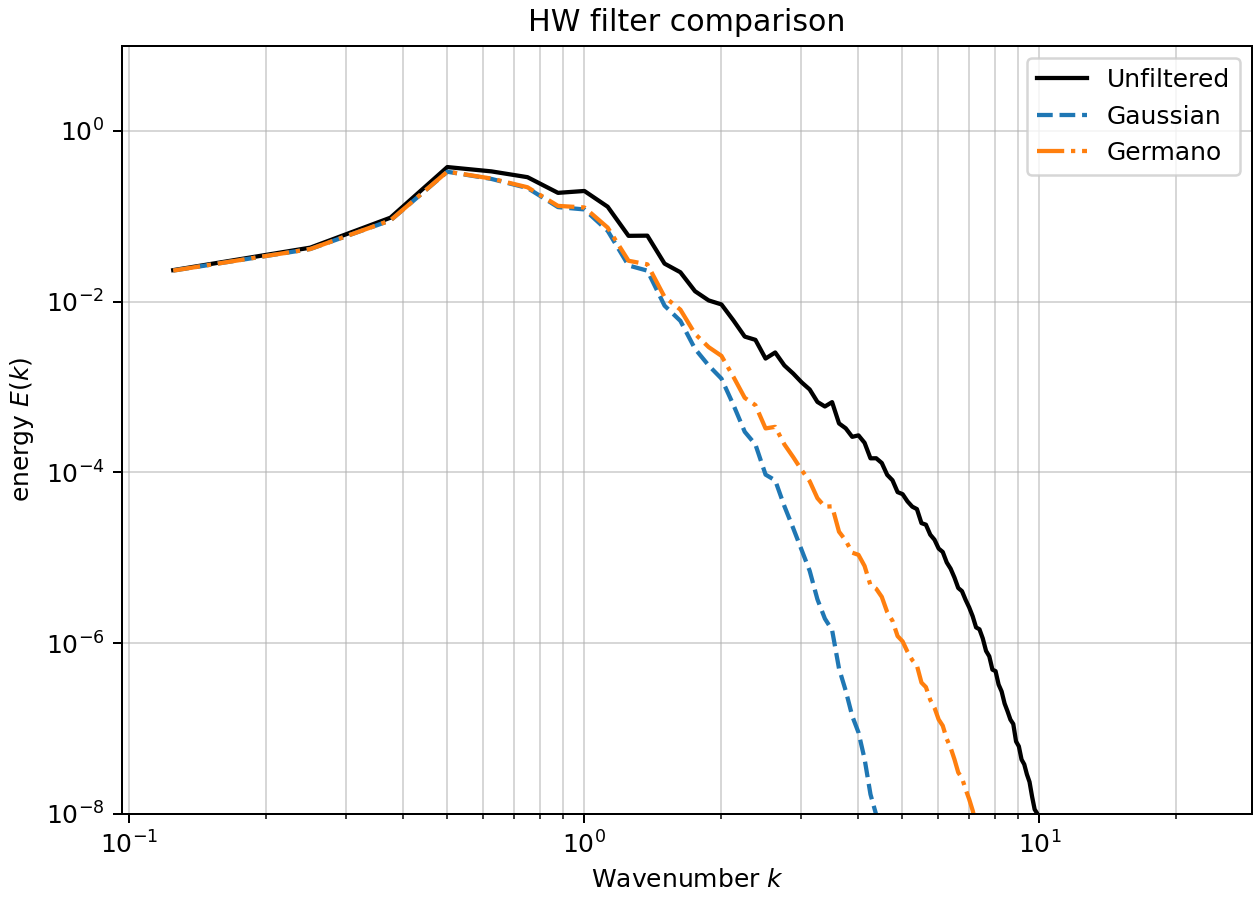
\includegraphics[width=0.85\linewidth]{images/fields_HW_run0_time501_N256_filter_spectra.png}
\caption{Energy spectra for the HW run-0 snapshot at $t=501$ on a $256^2$ mesh, comparing the unfiltered field with Gaussian and Germano filtering. Both filters attenuate the high-wavenumber spectrum; the Gaussian-filtered spectrum falls more steeply than the Germano-filtered spectrum in the plotted comparison.}
\label{fig:hw_filter_spectra}
\end{figure}

For homogeneous $\ell$ on the periodic domain, filtering is linear and commutes with spatial derivatives and the time derivative. Therefore, the filtering procedure satisfies the criteria for LES filtering of linearity, conservation and commutation \citep{sagaut_large_2006}. 
It also commutes with the poloidal average defining the mHW coupling. 
These properties justify filtering the linear terms directly. However, this cannot be assumed for spatially varying filter widths or incompatible boundary treatments \citep{klein2020commutation}. 

Applying the filter, $\mathcal{F}_\ell$, to \eqref{eq:hw_vorticity}--\eqref{eq:hw_density} (omitting the filtered mHW equations for brevity) yields
\begin{align}
    \partial_t\widetilde\zeta+\{\widetilde\phi,\widetilde\zeta\}
    &=\alpha(\widetilde\phi-\widetilde n)
      -\tau_{\mathrm{SGS},\zeta}-D_\zeta\nabla_\perp^4\widetilde\zeta,
    \label{eq:filtered_hw_vorticity}\\
    \partial_t\widetilde n+\{\widetilde\phi,\widetilde n\}
    &=\alpha(\widetilde\phi-\widetilde n)
      -\tau_{\mathrm{SGS},n}-\kappa\partial_y\widetilde\phi
      -D_n\nabla_\perp^4\widetilde n.
    \label{eq:filtered_hw_density}
\end{align}
where the exact nonlinear residual is
\begin{equation}
    \tau_{\mathrm{SGS},f}
    =\mathcal{F}_\ell\{\phi,f\}-\{\widetilde\phi,\widetilde f\},
    \qquad f\in\{n,\zeta\}.
    \label{eq:sgs_bracket}
\end{equation}
where the first term is calculated with our learned reconstruction. 
\todo{at this point, it is unclear what the need for the UNet is to me}

A central result of \citet{germano_differential_1986} is that the differential inverse gives exact expressions for filtered correlations. For two smooth scalar fields $a$ and $b$, define $C_\ell(a,b)=\mathcal{F}_\ell(ab)-\widetilde a\widetilde b$. The product rule and Eq.~\eqref{eq:germano_inverse} give
\begin{equation}
    \mathcal{H}_\ell C_\ell(a,b)
    =2\ell^2\nabla_\perp\widetilde a\cdot\nabla_\perp\widetilde b
     +\ell^4(\nabla_\perp^2\widetilde a)(\nabla_\perp^2\widetilde b).
    \label{eq:germano_correlation}
\end{equation}
Consequently, the exact correlation is the forward filter of the right-hand side, rather than just its leading gradient term. Applied to the two products in the Poisson bracket, this identity gives
\begin{equation}
    \tau_{\mathrm{SGS},f}
    =C_\ell(\partial_x\phi,\partial_y f)
     -C_\ell(\partial_y\phi,\partial_x f).
\end{equation}
Equivalently, the nonlinear term can be evaluated by reconstructing both fields:
\begin{equation}
    \mathcal{F}_\ell\{a,b\}
    =\mathcal{F}_\ell\{
       \mathcal{H}_\ell\widetilde a,
       \mathcal{H}_\ell\widetilde b\}.
    \label{eq:germano_bracket_inverse}
\end{equation}
where $a=\phi$ and $b$ is $n$ or $\zeta$.

These are continuous identities, not a closure assumption or a guarantee of exact reconstruction from coarse samples. As Germano emphasizes, an exactly inverted filtered system is formally a change of dependent variables; numerical resolution still limits the information retained.

In particular, the physical filter and the downsampling to the LES mesh are separate operations. Writing $\mathcal{R}_h$ for Fourier downsampling to that mesh, the network input is $(n,\phi)_{\mathrm{LES}}=\mathcal{R}_h\mathcal{F}_\ell(n,\phi)_{\mathrm{DNS}}$. Downsampling discards modes that the differential inverse alone cannot restore. Our learned reconstruction supplies an estimate of the filtered field on the fine mesh before inversion:
\begin{equation}
    (\widetilde{n},\widetilde{\phi})_{\mathrm{LES}}
    \xrightarrow{\mathcal{N}_\theta}
    (\widetilde n^{\mathrm{pred}},\widetilde\phi^{\mathrm{pred}})_{\mathrm{fDNS}}
    \xrightarrow{\mathcal{H}_\ell}
    (n^{\mathrm{rec}},\phi^{\mathrm{rec}})_{\mathrm{DNS}}.
    \label{eq:germano_learning_path}
\end{equation}
The inverse multiplier grows as $|\mathbf{k}|^2$, amplifying high-wavenumber prediction errors. The implementation therefore permits spectral regularization before or after inversion; when enabled, it changes the reconstruction from the exact inverse in Eq.~\eqref{eq:germano_inverse}. Vorticity is derived consistently as $\zeta^{\mathrm{rec}}=\nabla_\perp^2\phi^{\mathrm{rec}}$. The reconstructed nonlinear terms are then filtered and restricted,
\begin{equation}
    \mathcal{F}_\ell\{\phi,f\}
    =\mathcal{R}_h\mathcal{F}_\ell
      \{\phi^{\mathrm{rec}},f^{\mathrm{rec}}\},
      \qquad f\in\{n,\zeta\}.
\end{equation}
providing the LES solver with an approximation to the filtered fine-grid advection. This separates the analytically defined Germano inverse from the learned recovery of information lost through mesh downsampling.
%----------------------------------------------------------------
%
%
%
%
%
%
%
%----------------------------------------------------------------
\section{Numerical Implementation}\label{sec:NumericalImplementation}
We describe here the numerical implementation details for the full methodology. The settings below refer to the HW reconstruction from $32^2$ LES $\to$ $256^2$ DNS; they are not assumed to apply to every resolution or modified-HW case, but give very good guidance for other configurations. The BOUT++ solver \citep{dudson_bout++_2009} is used for solving the filtered HW and mHW equations. The coefficients $D_\zeta$ and $D_n$ correspond to \texttt{Dvort} and \texttt{Dn} in the BOUT++ implementation. In the two-dimensional runs, the paper's poloidal coordinate $y$ corresponds to the code's $z$ coordinate. For further details, see the Hasegawa-Wakatani example in the BOUT++ repository.

\subsection{NN-Architecture}\label{sec:NN-Architecture}
We use a variation of the U-Net architecture \citep{ronneberger_u-net_2015} for the reconstruction model, hereafter referenced as \textbf{DirectUNetSR}. However, as the input is already at the LES coarse resolution, we have an asymmetric architecture with a small encoder followed by a decoder to upsample the input to the fine DNS resolution. Skip connections are only used at low levels as we found that they tend to introduce artifacts during time integration which eventually degrade the reconstruction quality and lead to very strong oscillations. The reconstruction configuration described here is the HW training run with a $256^2$ DNS mesh and a $32^2$ LES mesh.

The three coarse input channels are density, potential and vorticity, denoted by $\mathbf{U}=(n,\phi,\zeta)$. The network predicts two fine-grid filtered fields, $\widetilde n_\theta$ and $\widetilde\phi_\theta$,\todo{why $\theta$??} being the vorticity obtained from the Laplacian of the potential fields $\zeta=\nabla_\perp^2\phi$. The encoder begins with 96 feature channels on the $32^2$ input mesh and uses a 192-channel bottleneck on a $16^2$ mesh. A skip-connected decoder returns to $32^2$, followed by periodic bilinear upsampling stages reaching $64^2$, $128^2$ and $256^2$. Circular convolution padding and periodic interpolation preserve the domain topology. The model has 1,670,738 trainable parameters and no global input skip connection. Figure~\ref{fig:direct_unet_architecture} summarizes the network and its differentiable reconstruction path.

\begin{figure}[htbp]
\centering
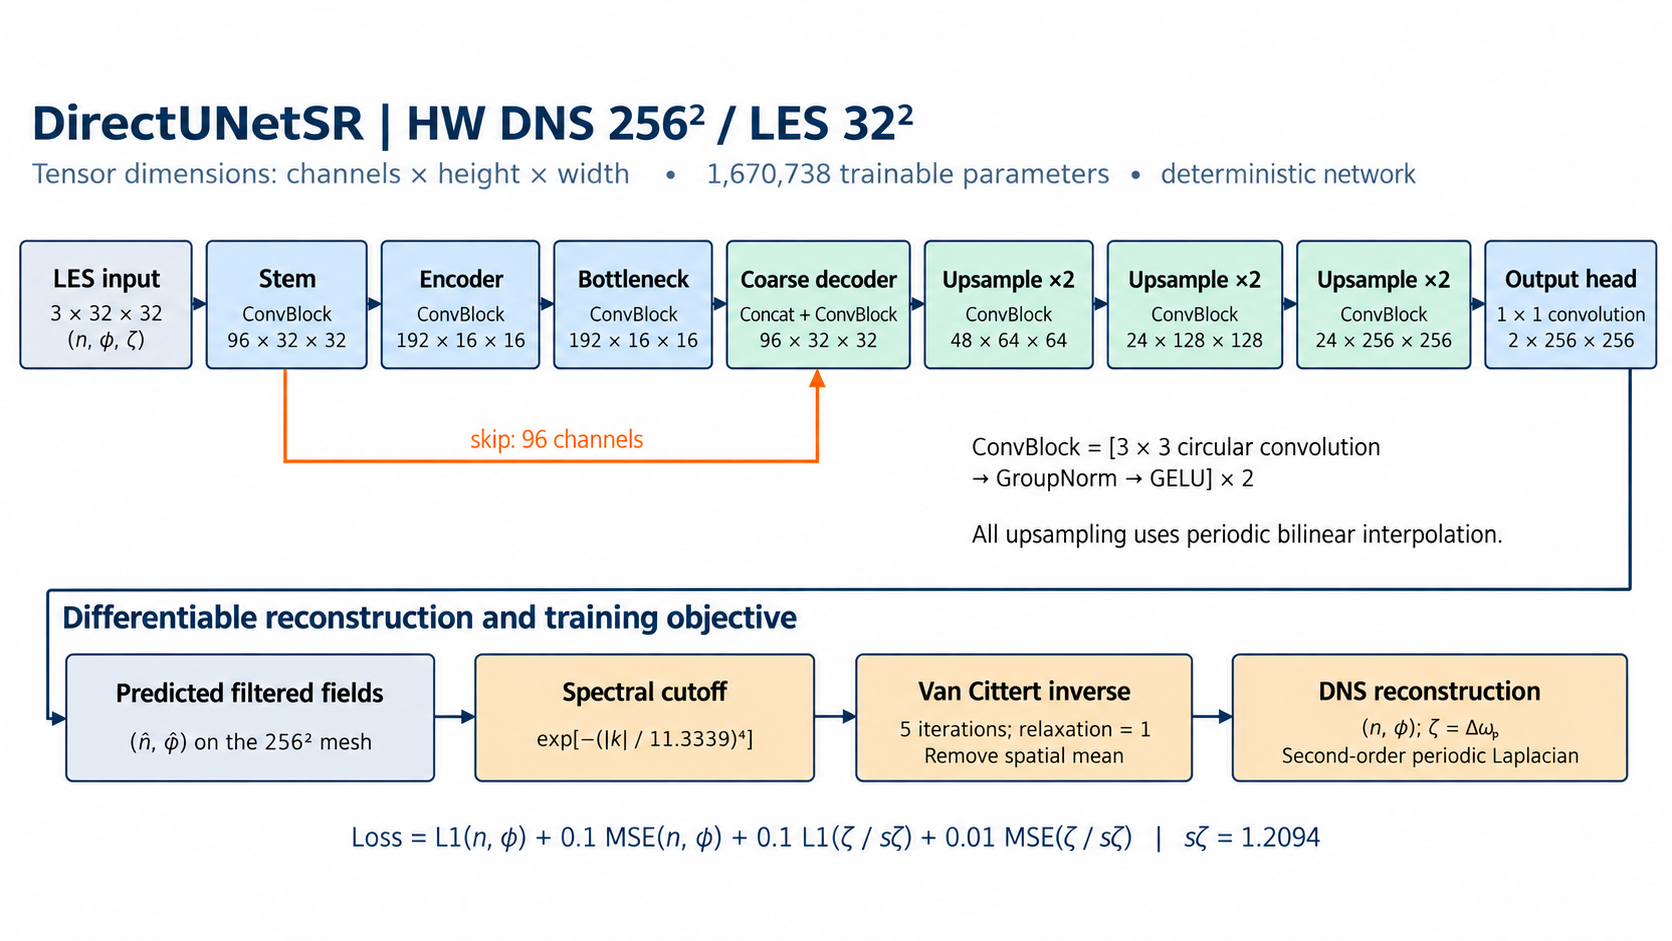
\includegraphics[width=\linewidth]{images/direct_unet_architecture2.png}
\caption{Current \texttt{DirectUNetSR} architecture for the HW $32^2$ LES $\to$ $256^2$ DNS training configuration. Tensor sizes are channels $\times$ height $\times$ width, omitting the batch dimension. The orange connection concatenates the stem features with the upsampled bottleneck features. Blue and green blocks contain learned convolutions; the spectral cutoff, van Cittert iterations and vorticity evaluation are fixed differentiable operations. The loss compares reconstructed fields with DNS targets; its vorticity terms use $\sigma_\zeta=1.2094$, and density/potential losses average both channels.}
\label{fig:direct_unet_architecture}
\end{figure}

\subsection{Reconstruction}
The output from the DirectUNetSR model is passed through a smooth spectral cutoff with multiplier to eliminate excessively high wavenumbers. The cutoff is configured to remove modes above the Nyquist frequency of the coarse LES mesh, with a smooth transition to avoid Gibbs oscillations. The cutoff multiplier is
\begin{equation}
    Q(\mathbf{k})=\exp\left[-\left(\frac{|\mathbf{k}|}{k_c}\right)^8\right],
    \qquad k_c=0.707107\,\frac{\pi}{h}\simeq11.3339.
\end{equation}
    \todo{where doesn the 0.707107 come from? Is it constant with downsampling factor?}
For stability purposes, the configured inverse is a truncated van Cittert reconstruction\todo{add reference}, rather than directly apply the inverse. For $g=Q\widetilde f_\theta$, implemented spectrally, it computes
\begin{equation}
    f^{(0)}=g,\qquad
    f^{(j+1)}=f^{(j)}+\omega\left[g-\mathcal{F}_\ell f^{(j)}\right],
    \quad j=0,\ldots,4,\qquad\omega=1.
    \label{eq:training_van_cittert}
\end{equation}
where $\omega$ is a relaxation parameter. The iteration is differentiable, and the network can learn to compensate for the approximate inverse. The reconstructed field is $f^{(5)}$ with its spatial mean removed to satisfy the divergence-free constraint on mass and electric charge. Thus this run uses five iterations of a regularized approximate inverse, rather than the exact differential inverse in Eq.~\eqref{eq:germano_inverse}. No post-inversion filter is enabled. Reconstructed vorticity is calculated from the potential using the second-order periodic finite-difference Laplacian,
\begin{equation}
    \zeta_\theta=\Delta_h\phi_\theta,\qquad
    (\Delta_h\phi)_{i,j}
    =\frac{\phi_{i+1,j}+\phi_{i-1,j}+\phi_{i,j+1}+\phi_{i,j-1}-4\phi_{i,j}}{h^2},
\end{equation}
with periodic indices. The DNS vorticity target is likewise derived from its potential.

\subsection{Loss function}
The objective function compares the reconstructed fields with DNS after cutoff, inversion and vorticity evaluation; gradients propagate through this entire path and it does not directly penalize the network's intermediate filtered output. Let:
\begin{equation}
    \overline{n}=\frac{n_\theta-n_{\mathrm{DNS}}}{\sigma_n},\qquad
    \overline{\phi}=\frac{\phi_\theta-\phi_{\mathrm{DNS}}}{\sigma_\phi},\qquad
    \overline{\zeta}=\frac{\zeta_\theta-\zeta_{\mathrm{DNS}}}{\sigma_\zeta},
\end{equation}
be the normalized reconstruction errors, where $f_\theta$ denotes the reconstructed field and $f_{\mathrm{DNS}}$ its DNS target. For each quantity $f\in\{n,\phi,\zeta\}$, $\sigma_f$ is the loss normalization scale, given by the training-data standard deviation when that normalization is enabled and otherwise by a unit scale. With $\mu_{B,\Omega}[q]$ denoting the statistical mean of $q$ over the batch and spatial grid, define
\begin{align}
    \mathcal{L}_{n\phi}^{(1)}
    &=\tfrac12\mu_{B,\Omega}\!\left[|\overline{n}|+|\overline{\phi}|\right],&
    \mathcal{L}_{n\phi}^{(2)}
    &=\tfrac12\mu_{B,\Omega}\!\left[\overline{n}^2+\overline{\phi}^2\right],\\
    \mathcal{L}_{\zeta}^{(1)}
    &=\mu_{B,\Omega}\!\left[|\overline{\zeta}|\right],&
    \mathcal{L}_{\zeta}^{(2)}
    &=\mu_{B,\Omega}\!\left[\overline{\zeta}^2\right].
\end{align}
the implemented loss is defined as:
\begin{align}
    \mathcal{L}
    &=\lambda_{n\phi}^{(1)}\mathcal{L}_{n\phi}^{(1)}
      +\lambda_{n\phi}^{(2)}\mathcal{L}_{n\phi}^{(2)}
      +\lambda_{\zeta}^{(1)}\mathcal{L}_{\zeta}^{(1)}
      +\lambda_{\zeta}^{(2)}\mathcal{L}_{\zeta}^{(2)}.
    \label{eq:training_loss}
\end{align}
where $\lambda_{n\phi}^{(1)}$, $\lambda_{n\phi}^{(2)}$, $\lambda_\zeta^{(1)}$ and $\lambda_\zeta^{(2)}$ denote the respective loss weights.

The density/potential terms average the two channels, so each coefficient weights their combined mean loss. The squared-error contribution increases the penalty on larger residuals, while the vorticity terms constrain potential curvature through the derived field.

\begin{table}[ht]
\centering
\caption{Loss settings recorded for the HW $256^2\rightarrow32^2$ training configuration. The four effective coefficients in Eq.~\eqref{eq:training_loss} correspond to the density/potential L1 and MSE weights and the vorticity L1 and MSE weights, respectively; the implementation forms the last coefficient as the product of its recorded vorticity and MSE weights.}
\label{tab:training_loss_weights}
\begin{tabular}{lll}
\toprule
Coefficient & Value & Role \\
\midrule
$\lambda_{n\phi}^{(1)}$ & 1.0 & Unit density/potential L1 prefactor \\
$\lambda_{n\phi}^{(2)}$ & 0.1 & Density/potential MSE weight \\
$\lambda_\zeta^{(1)}$ & 0.1 & Normalized vorticity L1 weight \\
$\lambda_\zeta^{(2)}$ & 0.01 & Normalized vorticity MSE weight \\
\bottomrule
\end{tabular}
\end{table}

\subsection{Numerical dataset}\label{sec:Dataset}

The DNS dataset were generated using the BOUT++ plasma solver, starting from the
Hasegawa-Wakatani input file provided in the examples folder. 
Table \ref{tab:cases}
and \ref{tab:dataset_effort} resumes the test case resolutions, physical parameters
and computational efforts from \citet{castagna_stylegan_2024}. Four configurations were analysed, two for the HW model and two for the mHW model, with $256^2$ and $512^2$ DNS meshes. The different dataset have a different final time $T_f$ but the same number of trajectories $N_{runs}$. We start collecting samples from $T_s$ every $\Delta T_s$ for a total $N_s$ samples. The choice of $\Delta T_s$ is such that the variation in Similarity Structural Index Metric (SSIM) is always $\geq$ 10\%. The last 2 columns of Table \ref{tab:dataset_effort} show the overall computational cost $C_{cost}$ in node per hours, where 1 node of ScafellPike supercomputer at Hartree Centre contains a 2 socket of 16-cores Intel Xeon Gold processors, and the disk space occupied by the data.

\begin{table}[htbp]
\centering
\caption{Physical parameters for each test case.}
\label{tab:cases}
\begin{tabular}{l|c c c c}
\hline
Type & $N$ & $\alpha$ & $\kappa$ & $\nu_\zeta=\nu_n$ \\
\hline
HW  & $256^2$ & 1 & 0.5 & $10^{-3}$ \\
HW  & $512^2$ & 1 & 1   & $10^{-4}$ \\
mHW & $256^2$ & 1 & 1   & $10^{-3}$ \\
mHW & $512^2$ & 1 & 1   & $10^{-4}$ \\
\hline
\end{tabular}
\end{table}

\begin{table}[htbp]
\centering
\caption{Computational cost and memory usage for each test case.}
\label{tab:dataset_effort}
\begin{tabular}{l|c c c c c c c c }
\hline
Type & $N$ & $T_s$ & $T_f$ & $\Delta T_s$ & $N_{\mathrm{runs}}$ & $N_s$ & $C_{\mathrm{cost}}$ & disk [GB] \\
\hline
HW  & $256^2$ & 501 & 1000 & 10 & 100 & 5000 & 5.8 & 7.4 \\
HW  & $512^2$ & 201 & 1000 & 10 & 100 & 8000 & 111 & 47 \\
mHW & $256^2$ & 201 & 400  & 4  & 100 & 5000 & 5.8 & 7.4 \\
mHW & $512^2$ & 201 & 400  & 4  & 100 & 5000 & 111 & 30 \\
\hline
\end{tabular}
\end{table}








\subsection{Training}\label{sec:Training}
We split the dataset into 80\% for training, 10\% for validation and the rest 10\% for testing.
The run for 100 epochs with batch size 4, using AdamW at a constant learning rate of $10^{-4}$, weight decay $10^{-6}$, moment coefficients $(0.9,0.999)$ and $\epsilon=10^{-8}$. Gradient norms are clipped to 1.0. Computation uses float64 precision on an NVIDIA H100 80GB GPU. Synchronized random periodic shifts augment the training fields while preserving alignment of inputs and targets.

Figure~\ref{fig:training_objective} shows the loss as function of number of epochs for the 
$32^2$ LES $\to$ $256^2$ DNS configuration. A rapid decrease in the total objective during the first 20 epochs, followed by a slower reduction throughout the remaining training. At epoch 100, the training and validation objectives are approximately $5.2\times10^{-2}$ and $5.6\times10^{-2}$, respectively. The validation curve closely follows the training curve initially and develops a small gap at later epochs, while continuing to decrease overall. This behaviour indicates diminishing gains from further optimization without a sustained increase in validation loss over the recorded interval.

\begin{figure}[htbp]
\centering
% Show only the Total Training Objective panel of the original 180-dpi summary.
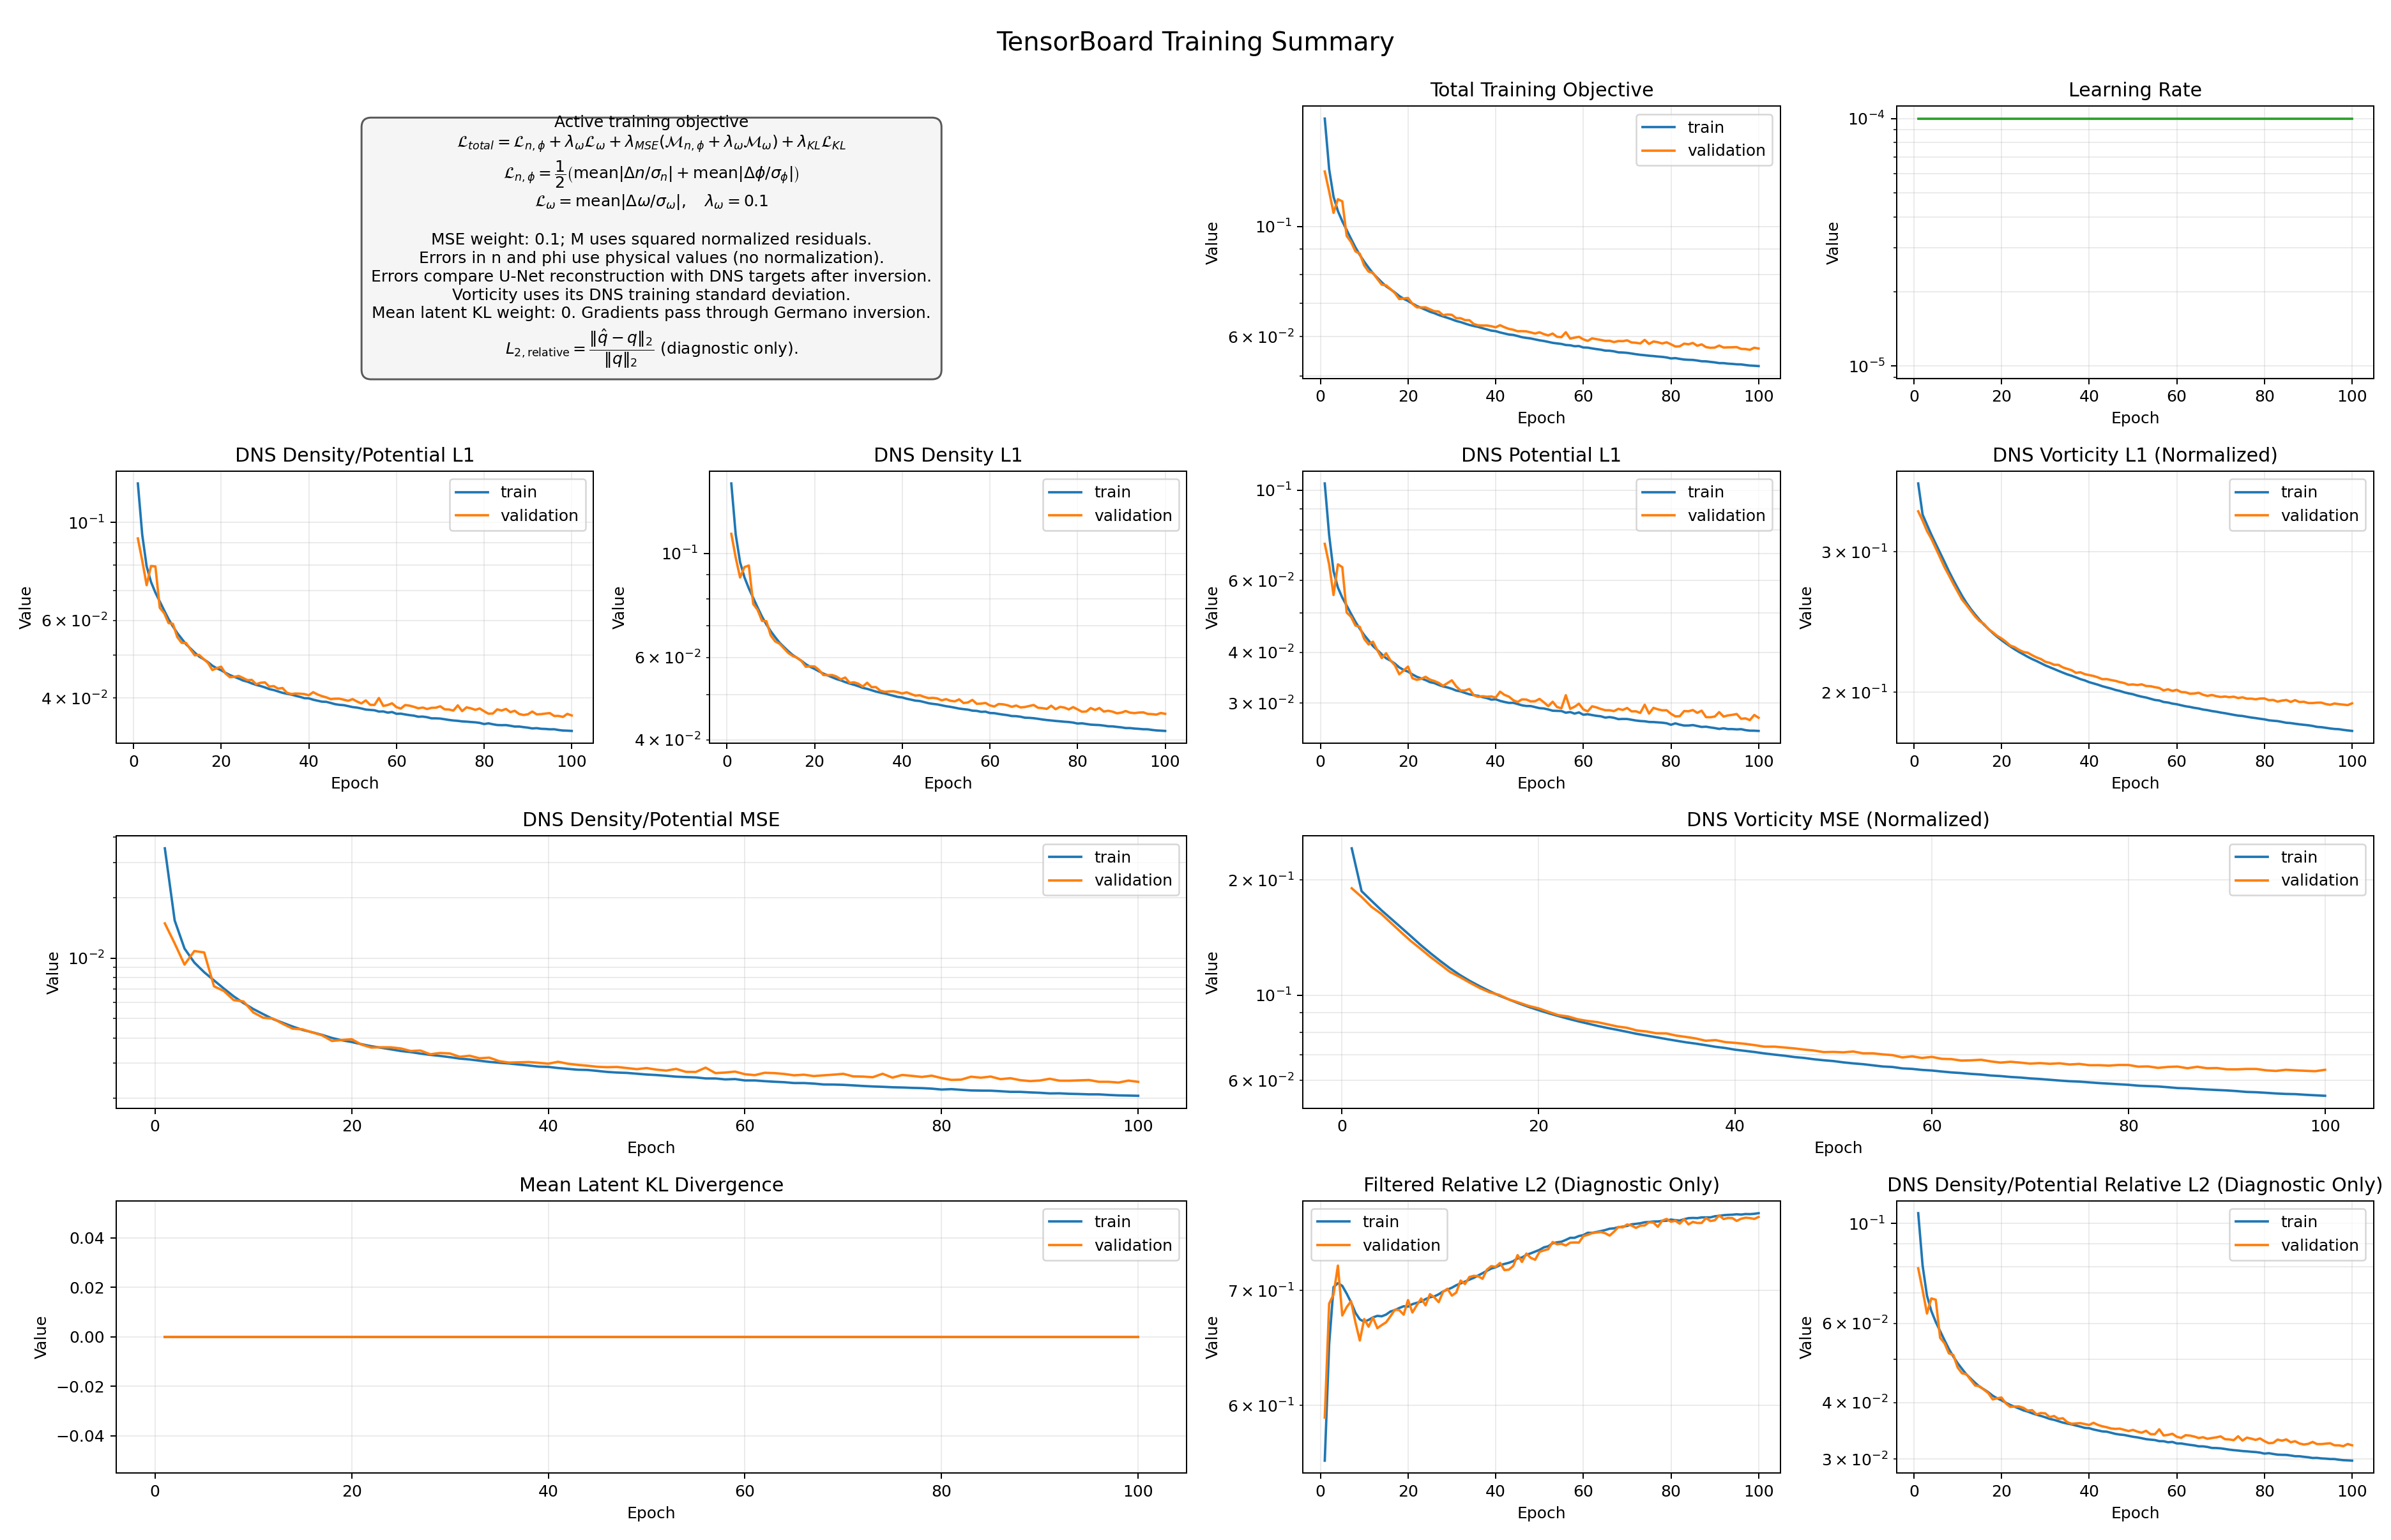
\includegraphics[width=0.75\linewidth,trim=736bp 688bp 372bp 42bp,clip]{images/HW_dns256_les32_tensorboard_summary.png}
\caption{Total training and validation objective, Eq.~\eqref{eq:training_loss}, for the HW configuration with $256^2$ DNS and $32^2$ LES grids over 100 epochs.}
\label{fig:training_objective}
\end{figure}


%----------------------------------------------------------------
%
%
%
%
%
%
%
%----------------------------------------------------------------
\section{Results}\label{sec:Results}

We compare HW and mHW at DNS resolutions of $256^2$ and $512^2$, each with three LES resolutions. The $256^2$ cases use $128^2$, $64^2$ and $32^2$ LES meshes; the $512^2$ cases use $256^2$, $128^2$ and $64^2$ meshes. These correspond to reductions by factors of two, four and eight in each direction. The updated HW diagnostics cover $0\leq t\leq1000$, whereas the mHW diagnostics cover $0\leq t\leq100$. The shorter mHW window reflects its faster dynamics and the tendency of the flow to laminarize beyond this interval. Endpoint statistics are evaluated at $t=0$ and the final time of each model; spatial comparisons remain at $t=0$.

The statistical figures show energy, enstrophy and particle-flux histories, endpoint spectra and three endpoint PDFs. The mHW\_N256 plots are regenerated from the DNS dumps and saved U-Net reconstructed fields for the $128^2$, $64^2$ and $32^2$ LES meshes, using the same $0\leq t\leq100$ window. The comparisons are against DNS; no separate conventional-closure curve is present. Approximate numerical values below are read from the plotted curves.

\subsection{Spatial reconstruction}

Figures~\ref{fig:fields-HW_N256}--\ref{fig:fields-mHW_N512} compare the initial density, potential and vorticity fields at $t=0$ for DNS and the two finer LES meshes. These comparisons assess the spatial fidelity of the initial reconstruction. The HW panels resolve vortex structures, while the mHW potential panels show bands extended in the poloidal direction. The signed difference panels, defined as DNS minus LES, identify local reconstruction errors in each field.

Only the initial spatial comparisons are shown here. They provide a qualitative assessment of reconstruction fidelity but do not establish dynamical accuracy or an integrated error norm. The subsequent evolution is assessed through the statistical diagnostics below. The coarsest LES meshes are included in those diagnostics, but are absent from the archived spatial comparison panels.

\begin{figure}[p]
\centering
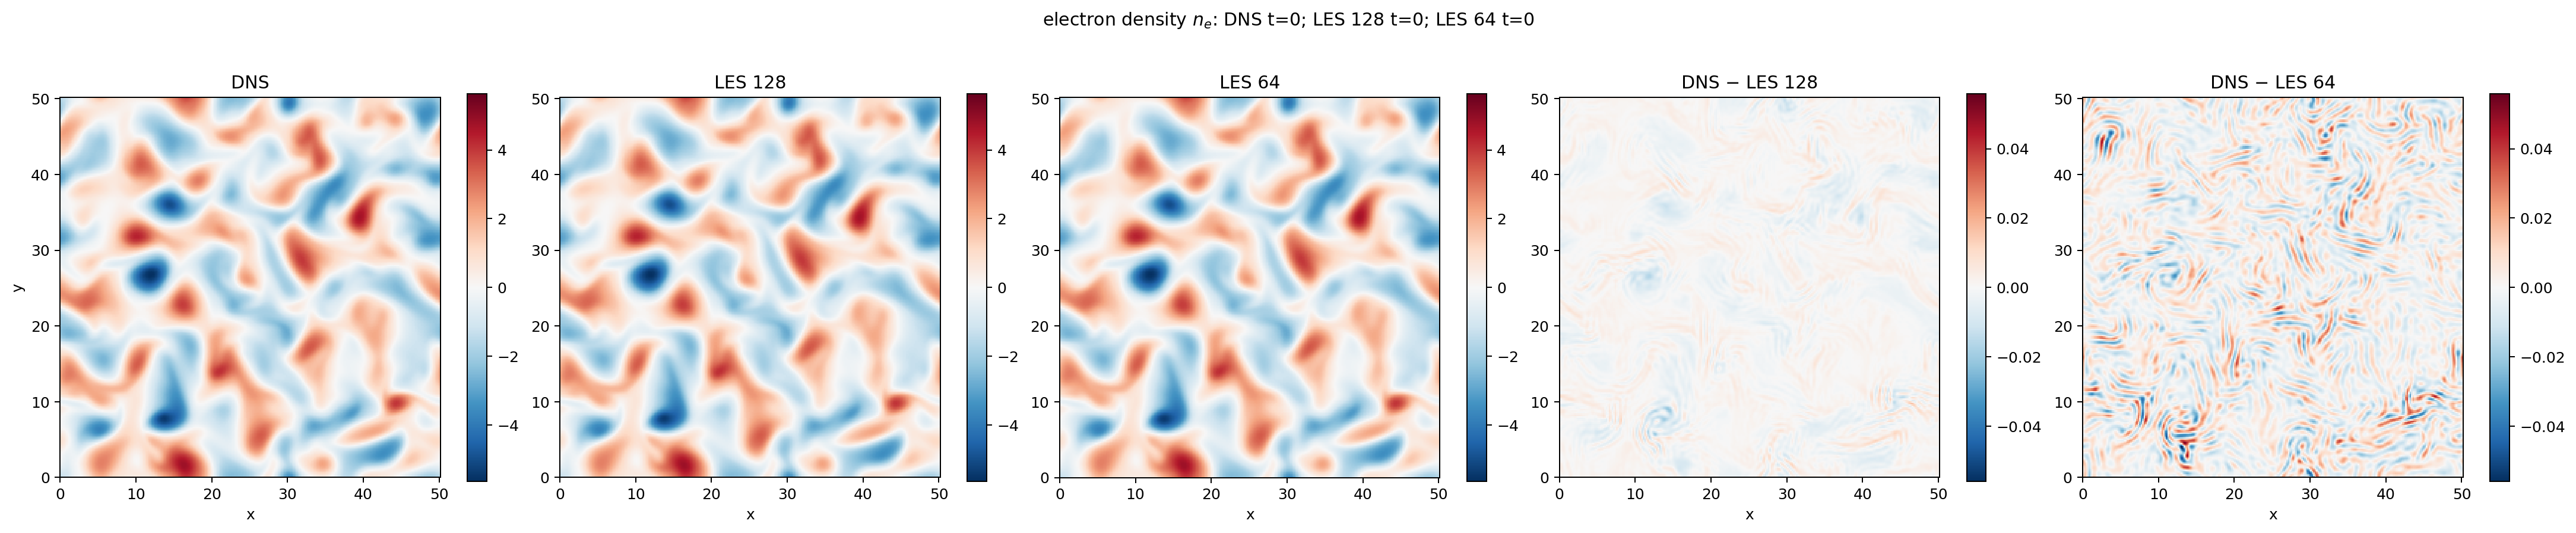
\includegraphics[width=\linewidth]{images/validation_current/HW_N256/U_comparison_frames/U_0000000.png}
\par\smallskip
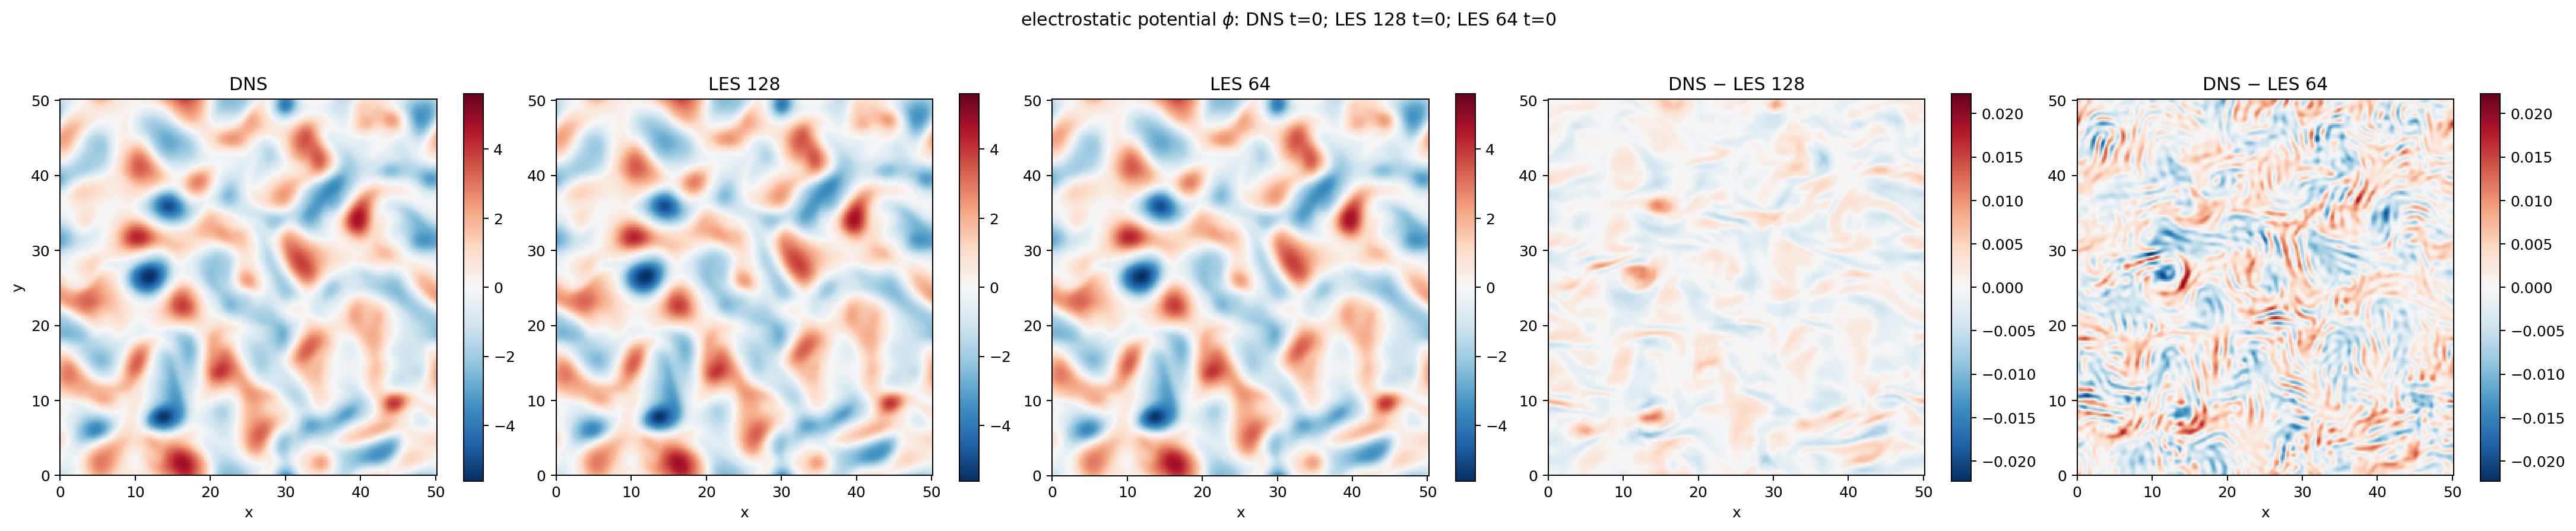
\includegraphics[width=\linewidth]{images/validation_current/HW_N256/V_comparison_frames/V_0000000.png}
\par\smallskip
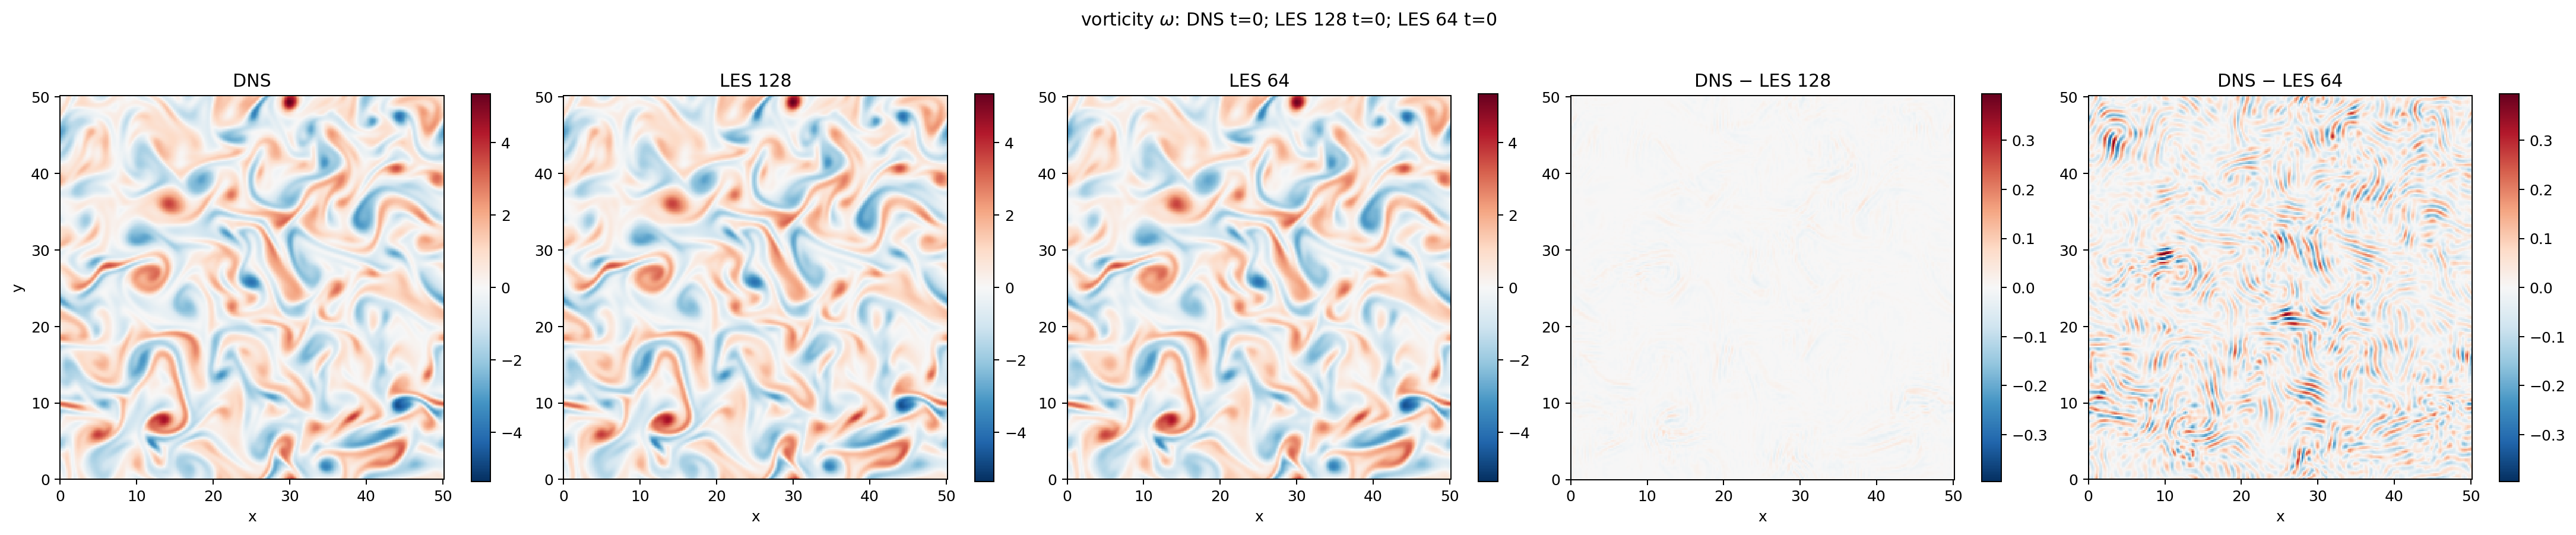
\includegraphics[width=\linewidth]{images/validation_current/HW_N256/P_comparison_frames/P_0000000.png}
\par\smallskip
\caption{HW\_N256 spatial comparisons at $t=0$: density (top), potential (middle) and vorticity (bottom). Each row shows DNS, the two finer LES reconstructions and their signed differences from DNS, as labelled. Signed differences are defined as DNS minus LES.}
\label{fig:fields-HW_N256}
\end{figure}

\begin{figure}[p]
\centering
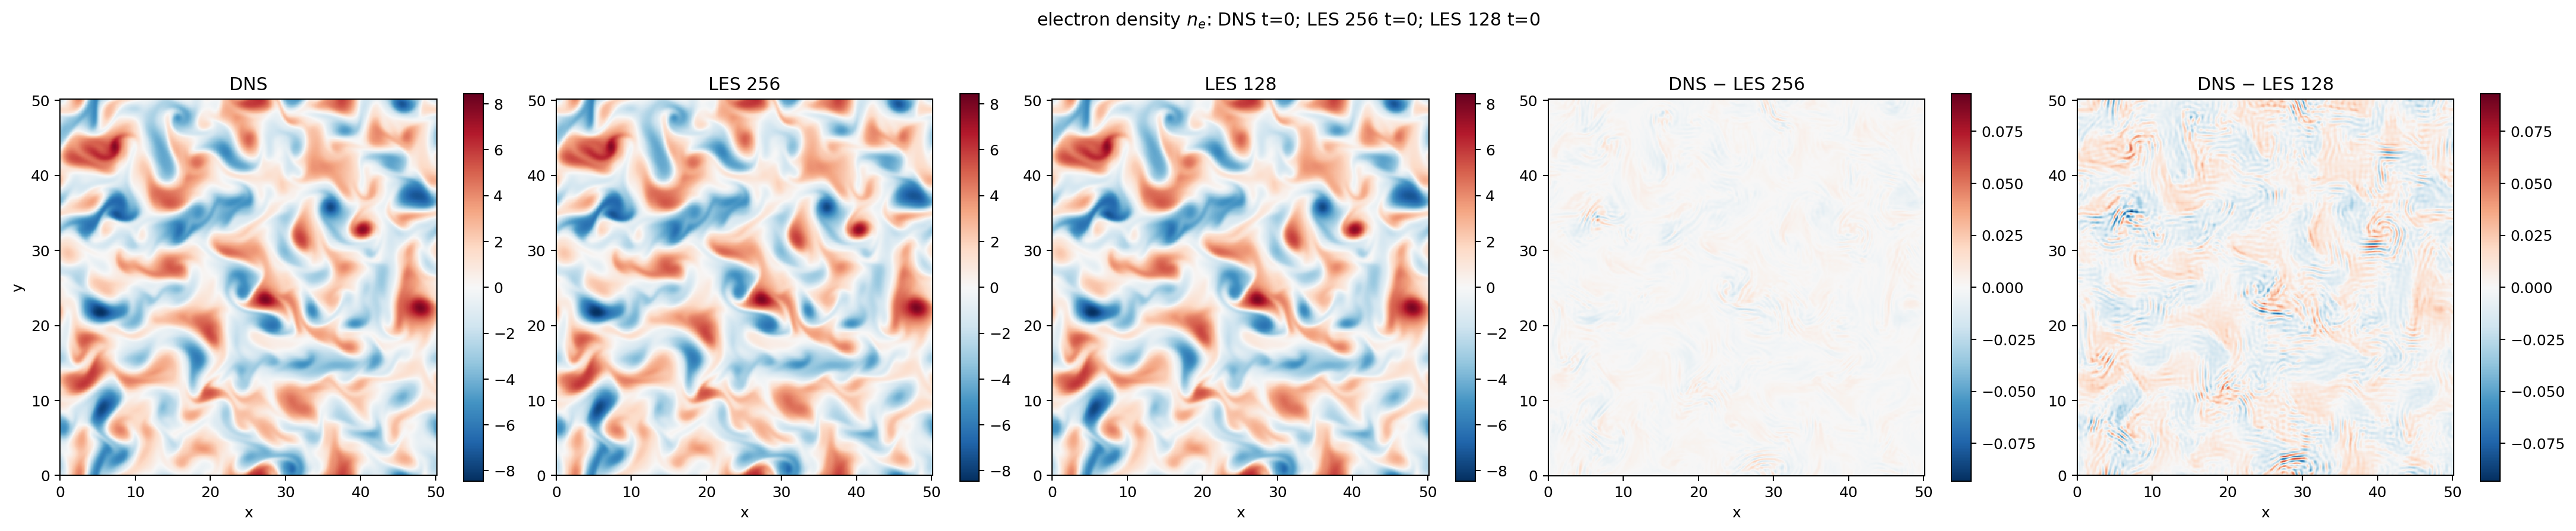
\includegraphics[width=\linewidth]{images/validation_current/HW_N512/U_comparison_frames/U_0000000.png}
\par\smallskip
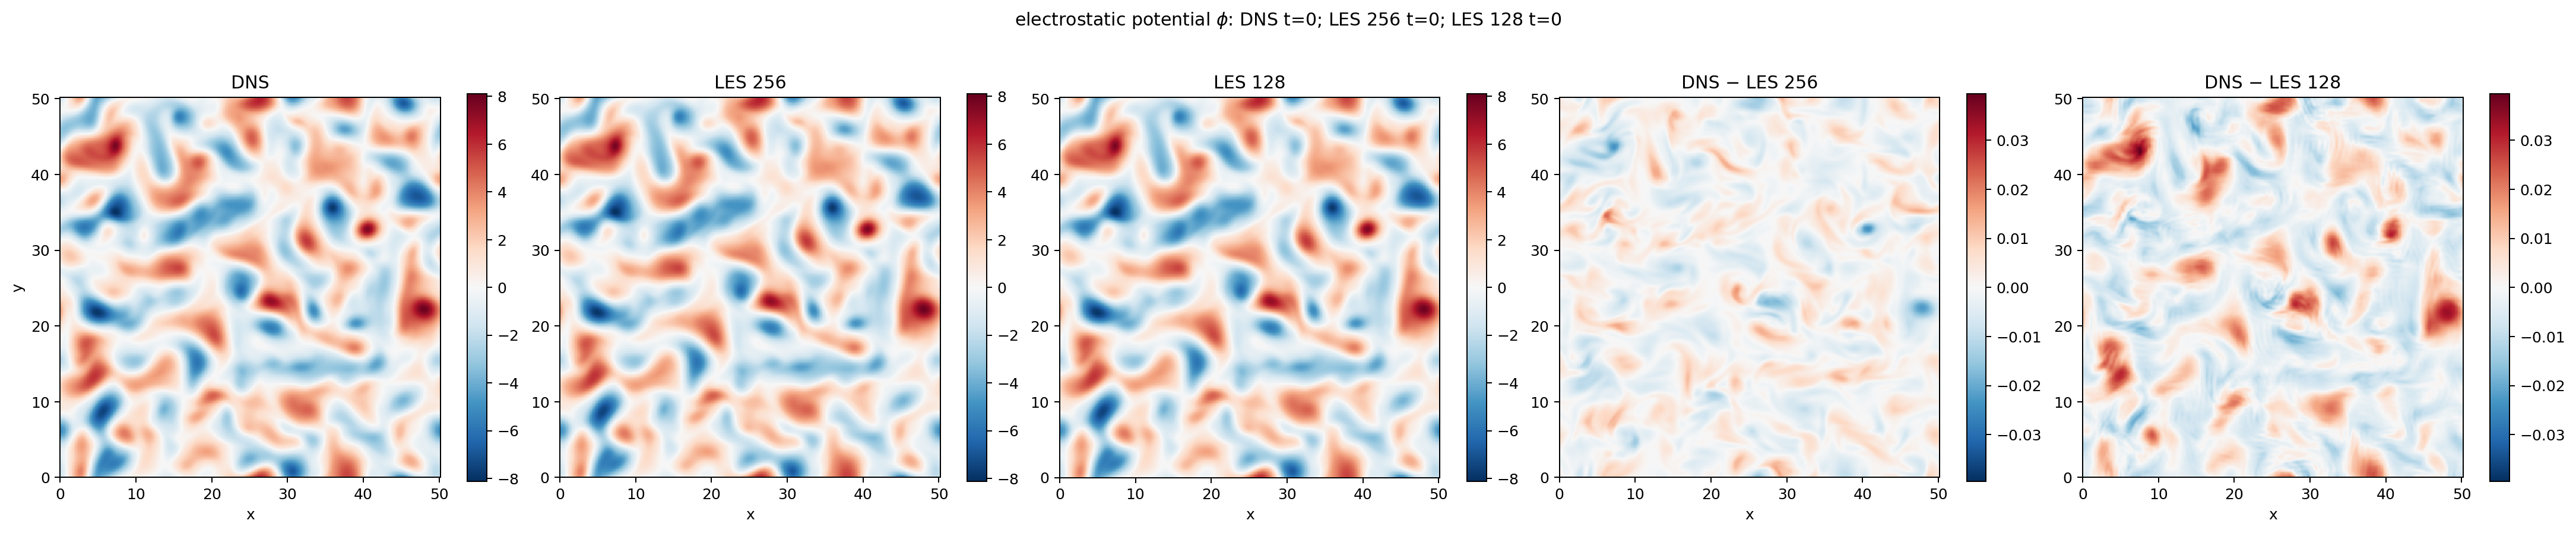
\includegraphics[width=\linewidth]{images/validation_current/HW_N512/V_comparison_frames/V_0000000.png}
\par\smallskip
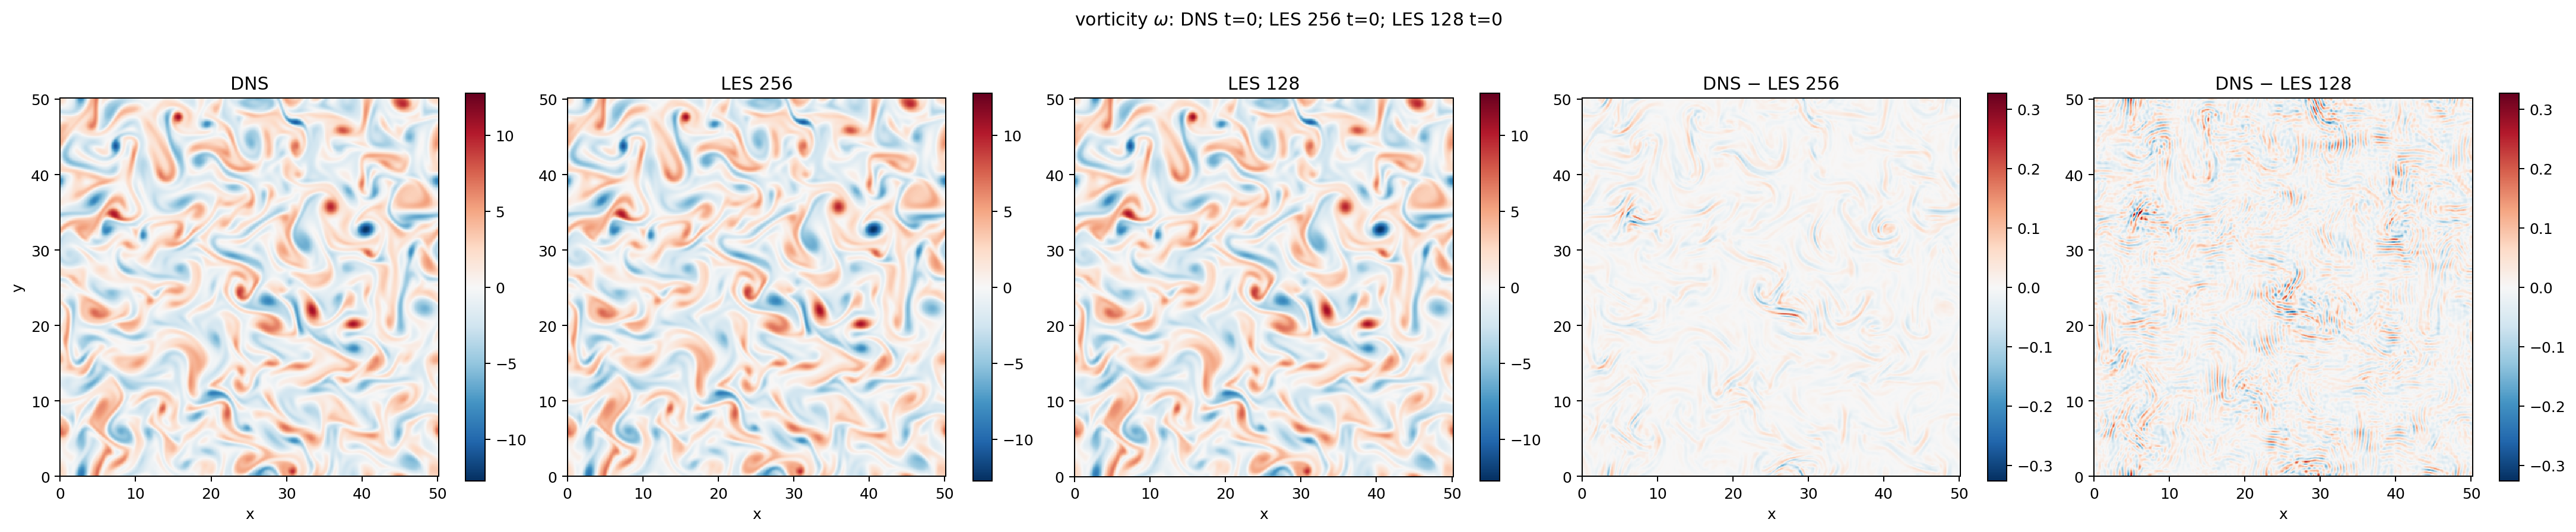
\includegraphics[width=\linewidth]{images/validation_current/HW_N512/P_comparison_frames/P_0000000.png}
\par\smallskip
\caption{HW\_N512 spatial comparisons at $t=0$: density (top), potential (middle) and vorticity (bottom). Each row shows DNS, the two finer LES reconstructions and their signed differences from DNS, as labelled. Signed differences are defined as DNS minus LES.}
\label{fig:fields-HW_N512}
\end{figure}

\begin{figure}[p]
\centering
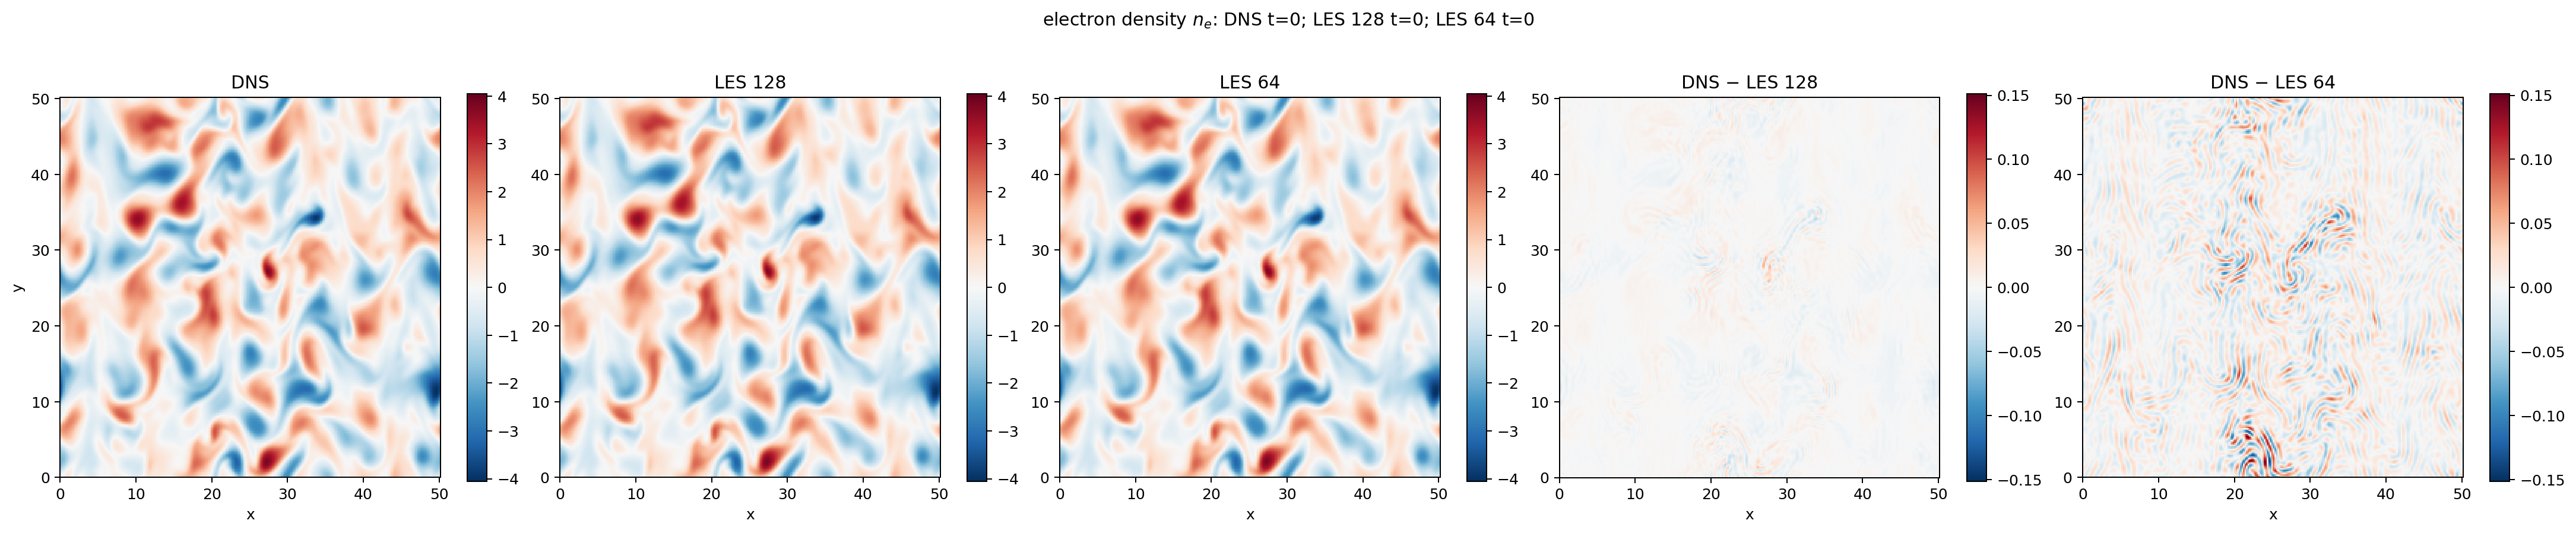
\includegraphics[width=\linewidth]{images/validation_current/mHW_N256/U_comparison_frames/U_0000000.png}
\par\smallskip
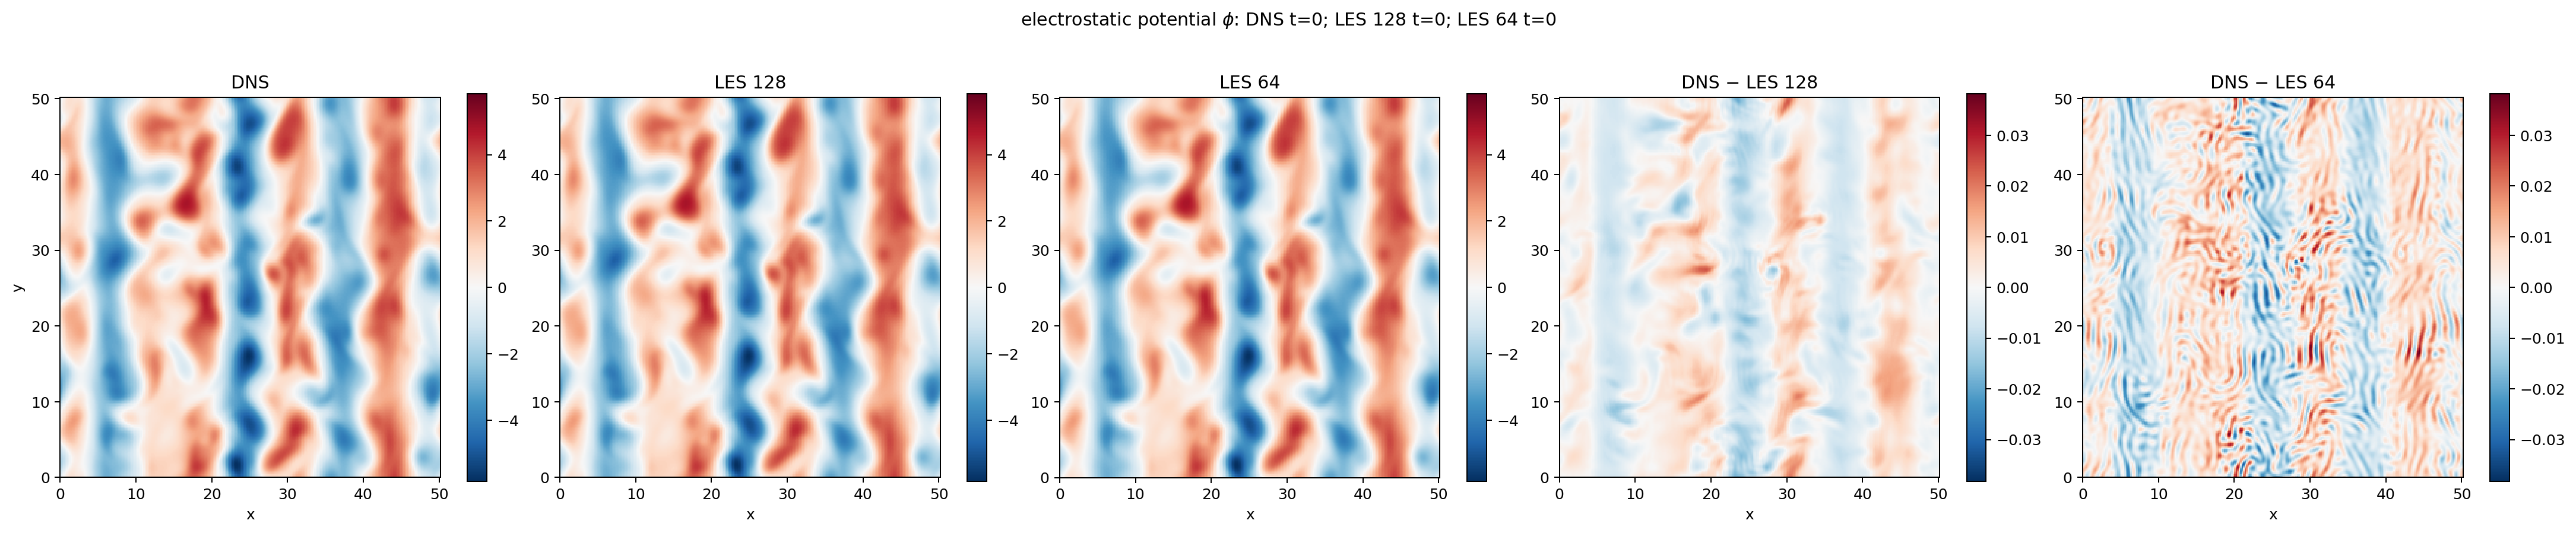
\includegraphics[width=\linewidth]{images/validation_current/mHW_N256/V_comparison_frames/V_0000000.png}
\par\smallskip
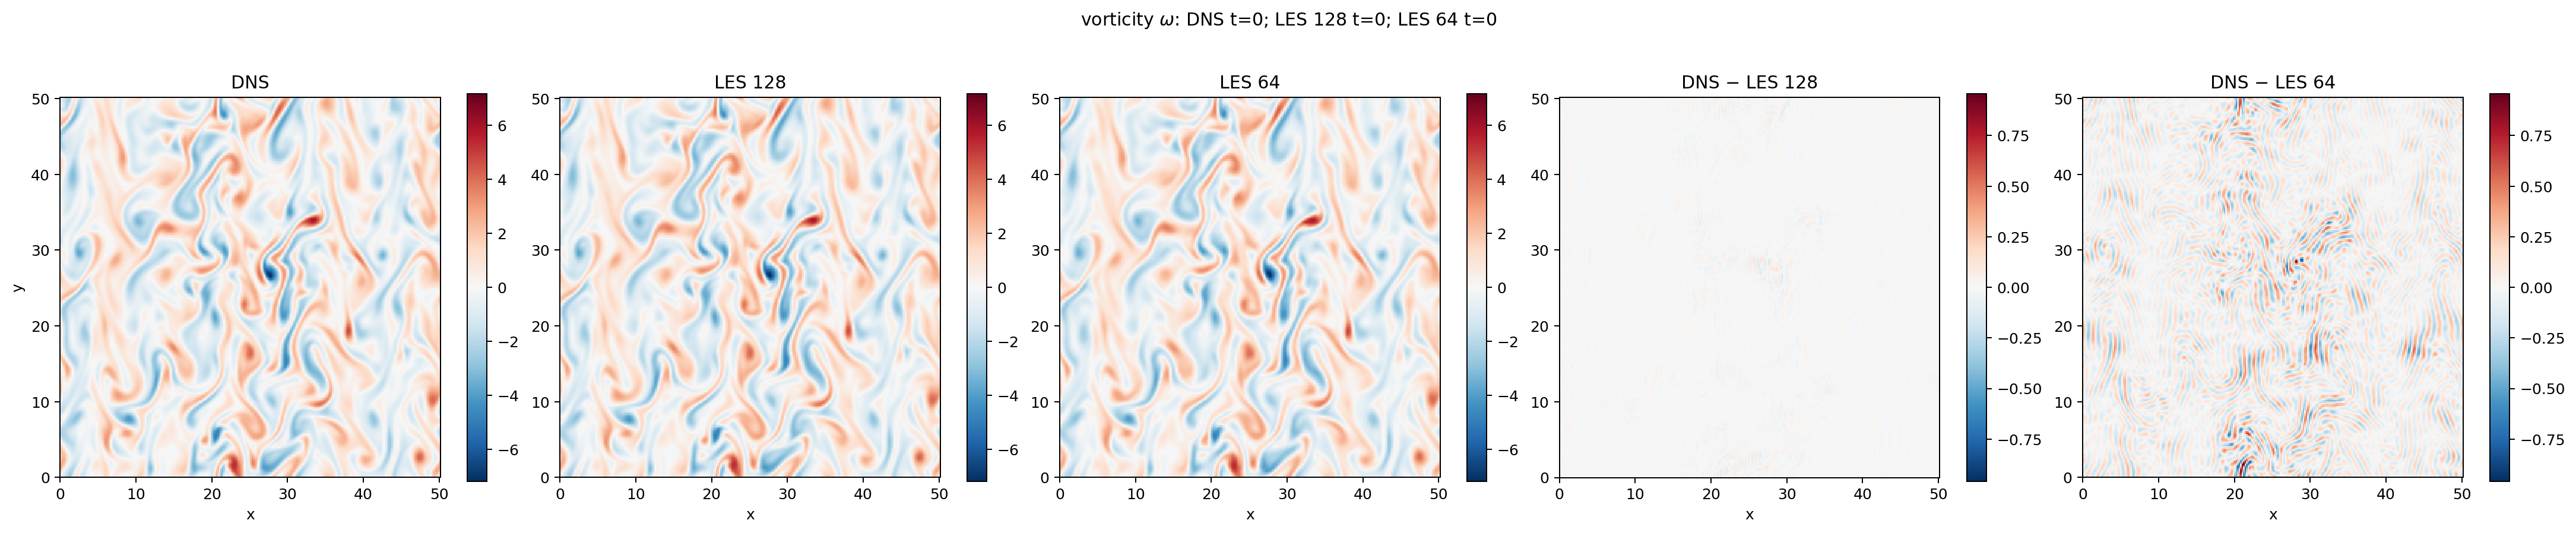
\includegraphics[width=\linewidth]{images/validation_current/mHW_N256/P_comparison_frames/P_0000000.png}
\par\smallskip
\caption{mHW\_N256 spatial comparisons at $t=0$: density (top), potential (middle) and vorticity (bottom). Each row shows DNS, the two finer LES reconstructions and their signed differences from DNS, as labelled. Signed differences are defined as DNS minus LES.}
\label{fig:fields-mHW_N256}
\end{figure}

\begin{figure}[p]
\centering
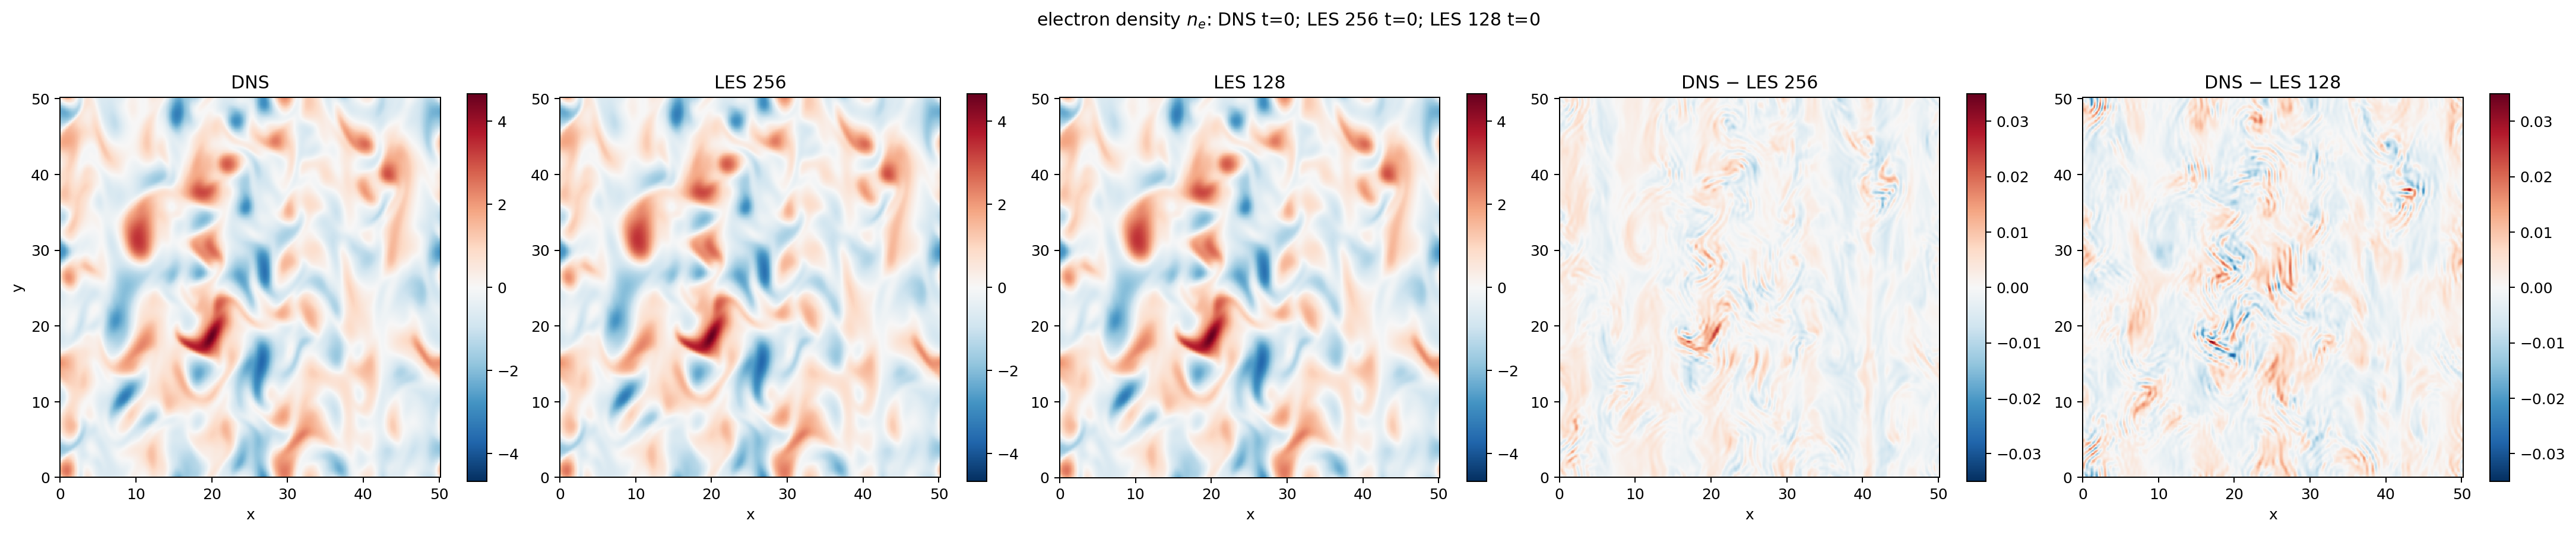
\includegraphics[width=\linewidth]{images/validation_current/mHW_N512/U_comparison_frames/U_0000000.png}
\par\smallskip
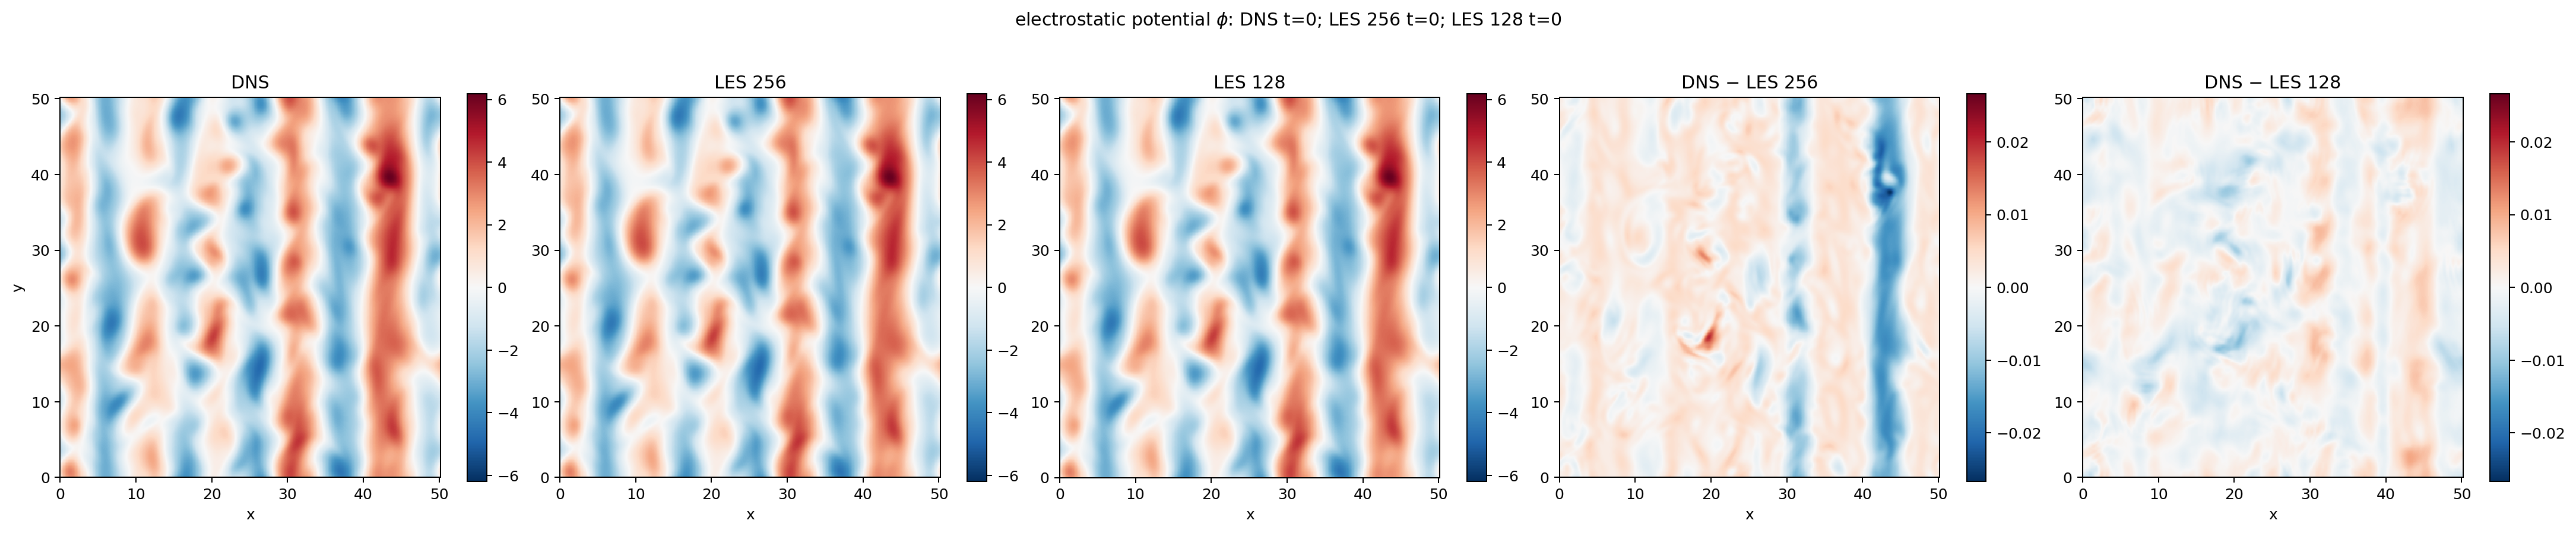
\includegraphics[width=\linewidth]{images/validation_current/mHW_N512/V_comparison_frames/V_0000000.png}
\par\smallskip
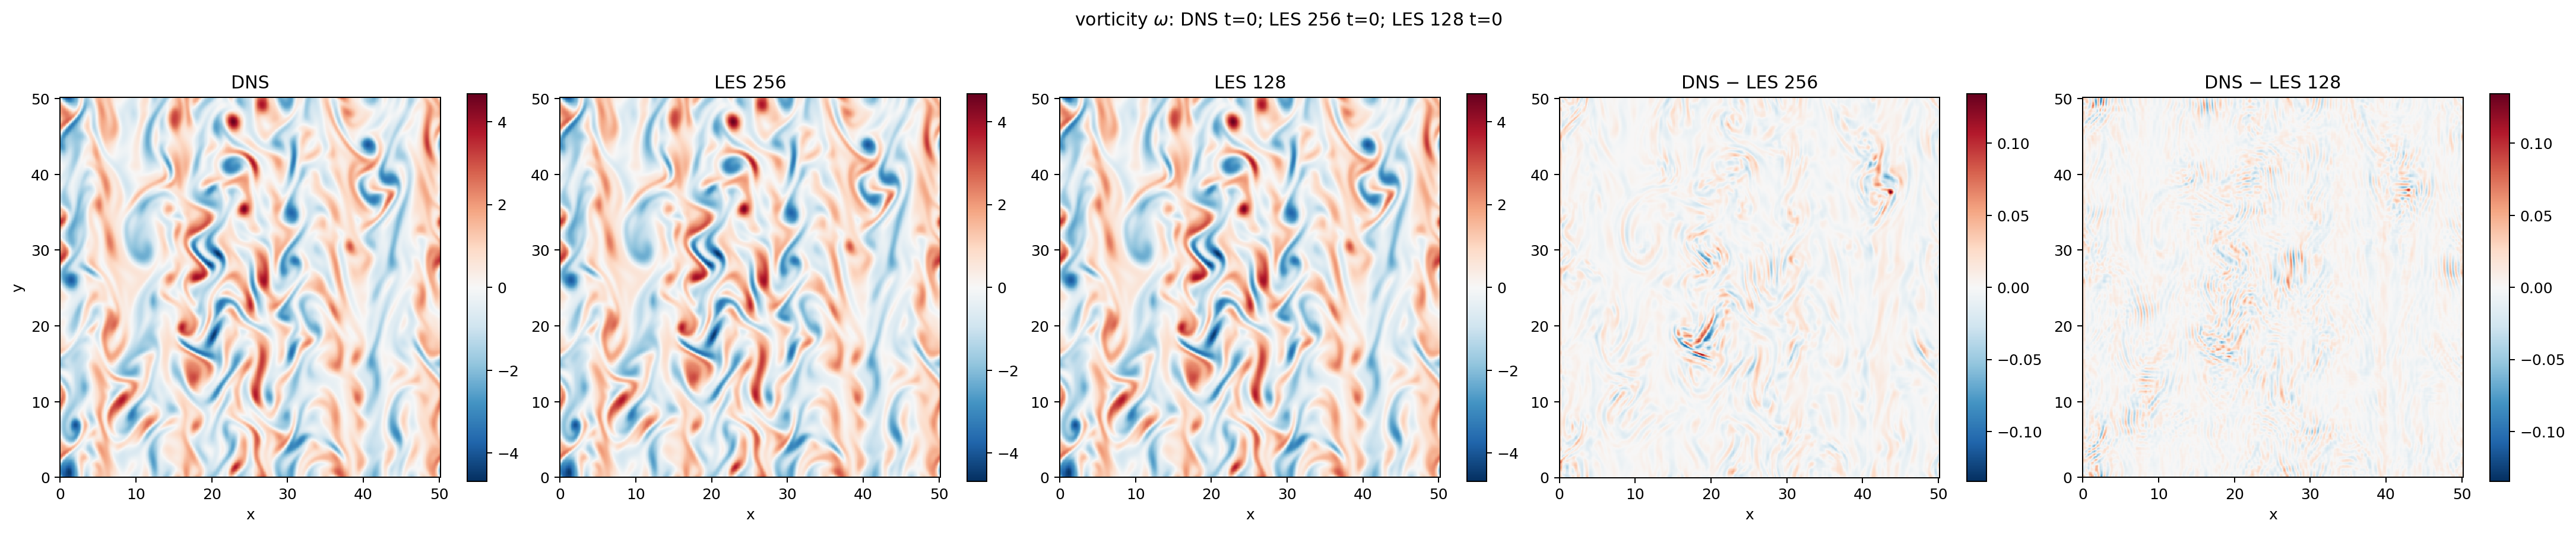
\includegraphics[width=\linewidth]{images/validation_current/mHW_N512/P_comparison_frames/P_0000000.png}
\par\smallskip
\caption{mHW\_N512 spatial comparisons at $t=0$: density (top), potential (middle) and vorticity (bottom). Each row shows DNS, the two finer LES reconstructions and their signed differences from DNS, as labelled. Signed differences are defined as DNS minus LES.}
\label{fig:fields-mHW_N512}
\end{figure}

\subsection{Energy and enstrophy}

The diagnostics are the spatially integrated HW energy and generalized enstrophy,
\begin{align}
 E &= \frac12\int_\Omega\left(n^2+|\nabla_\perp\phi|^2\right)\,d\mathbf{x},\\
 W &= \frac12\int_\Omega(n-\zeta)^2\,d\mathbf{x}.
\end{align}
The current plotting routine evaluates both with cell-area quadrature:
\begin{align}
 E_h &= \frac{\Delta x\Delta y}{2}\sum_{i,j}
 \left[n_{ij}^2+(D_x\phi)_{ij}^2+(D_y\phi)_{ij}^2\right],\\
 W_h &= \frac{\Delta x\Delta y}{2}\sum_{i,j}(n_{ij}-\zeta_{ij})^2,
\end{align}
where $D_x$ and $D_y$ are fourth-order periodic finite-difference derivatives. The plots label generalized enstrophy as $Z$ and vorticity as $\omega$; these correspond to $W$ and $\zeta$ here.

Figures~\ref{fig:energy} and~\ref{fig:enstrophy} reveal a strong resolution dependence over the longer HW interval. In HW\_N256, DNS energy fluctuates around $4.1$--$5.4\times10^3$. The $128^2$ and $64^2$ LES meshes retain comparable energy levels, although their fluctuations do not remain synchronized with DNS. The $32^2$ LES instead decays rapidly to approximately $1.0$--$1.3\times10^3$ after $t\simeq150$. Its generalized enstrophy falls to roughly $2.5$--$3.0\times10^3$, compared with DNS levels of approximately $7.5$--$9.5\times10^3$. Thus the coarse reconstruction loses both diagnostics over the longer interval.

For HW\_N512, DNS energy is typically $1.4$--$1.7\times10^4$, with intermittent larger excursions. The $256^2$ LES retains this range, while $128^2$ generally lies lower and $64^2$ remains near $1.1$--$1.4\times10^4$. Enstrophy shows a similar ordering: the coarsest curve is mostly around $2.3$--$2.9\times10^4$, below the DNS range of roughly $2.9$--$3.8\times10^4$. Agreement here concerns fluctuation levels and statistical behaviour rather than pointwise tracking of the turbulent trajectory.

For mHW\_N256, DNS energy rises from approximately $3.55\times10^3$ to $4.33\times10^3$ near $t=30$, before declining to $3.86\times10^3$ at $t=100$. The $128^2$ and $64^2$ reconstructions end near $3.86\times10^3$ and $3.90\times10^3$, respectively. The $32^2$ reconstruction instead continues growing to $5.23\times10^3$. Its generalized enstrophy reaches $8.81\times10^3$, compared with $3.51\times10^3$ for DNS and $3.54\times10^3$ and $3.76\times10^3$ for the two finer meshes. Thus the coarsest reconstruction fails to reproduce the decay and develops excess enstrophy well before the end of the mHW validation window.

In mHW\_N512, DNS energy initially rises from approximately $3.3\times10^3$ to $3.6\times10^3$ near $t=12$--$15$, then falls to about $3.0\times10^3$ at $t=100$. Generalized enstrophy similarly peaks near $5.4\times10^3$ before declining to about $2.7\times10^3$. The $256^2$ LES closely follows both trends. The $128^2$ and $64^2$ energy curves end near $2.9\times10^3$ and $2.75\times10^3$, respectively, with corresponding enstrophy deficits. This decay is consistent with the progression toward laminarization motivating the shorter mHW validation window.

\begin{figure}[p]
\centering
\begin{subfigure}[t]{0.48\textwidth}
\centering
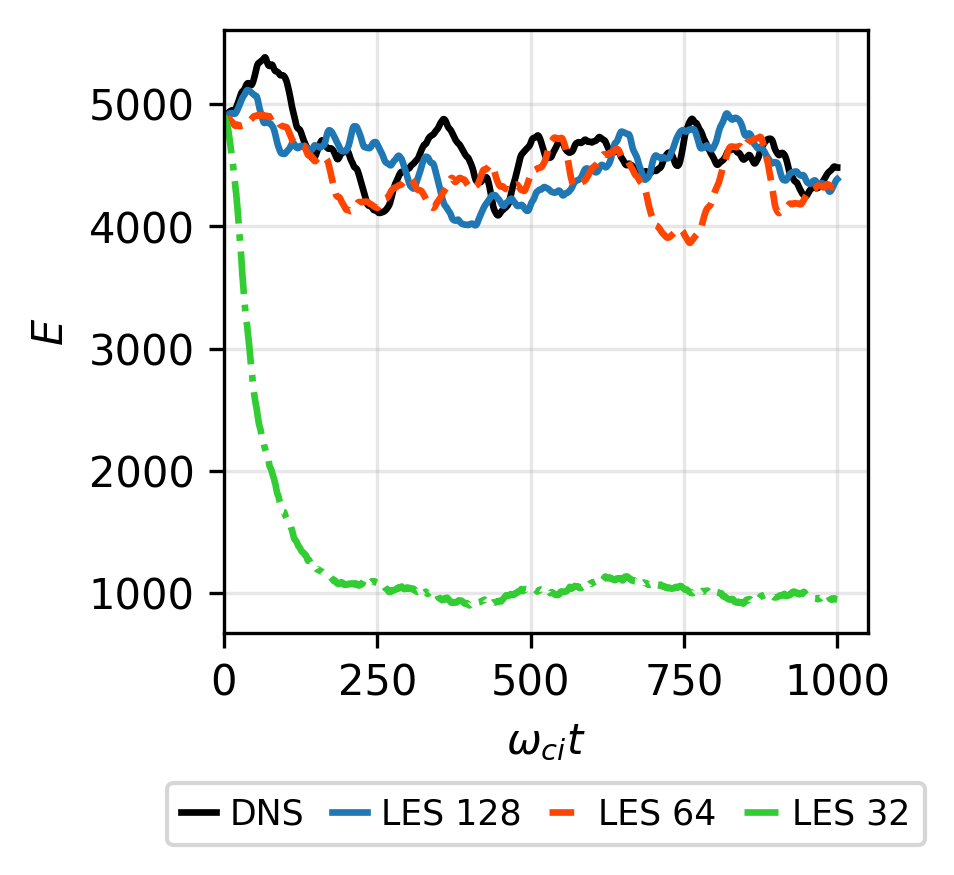
\includegraphics[width=\linewidth]{images/validation_current/HW_N256/energy_vs_time.png}
\caption{HW\_N256}
\end{subfigure}
\hfill
\begin{subfigure}[t]{0.48\textwidth}
\centering
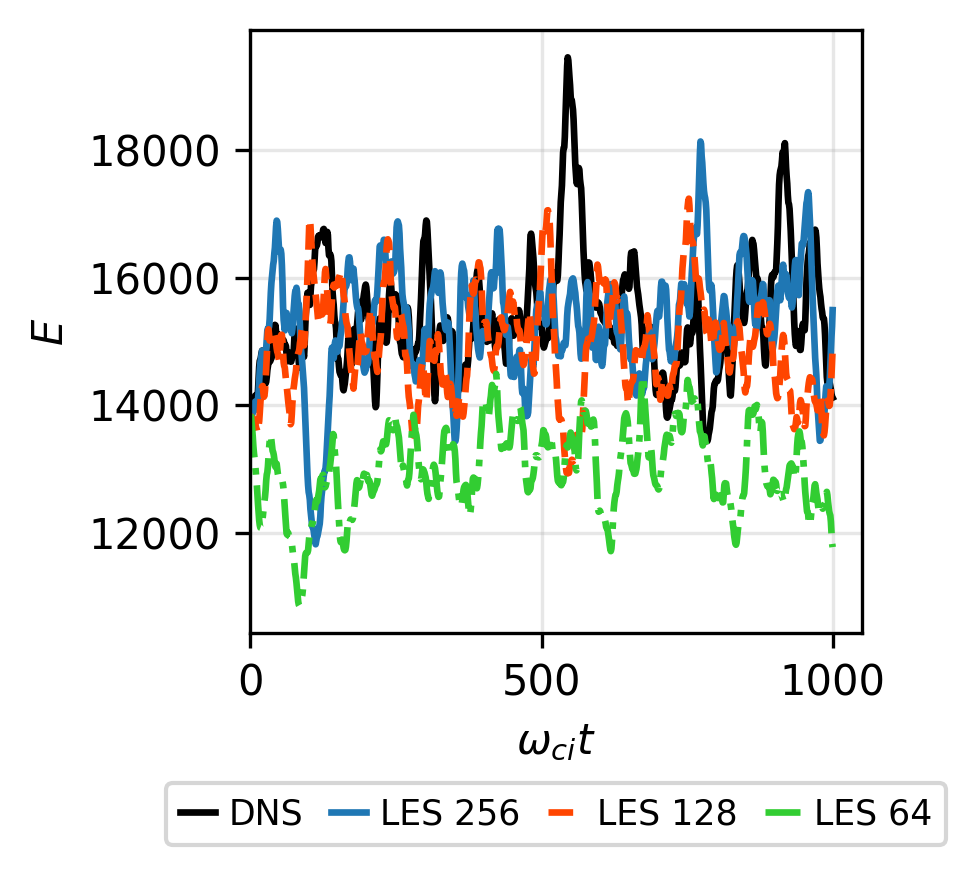
\includegraphics[width=\linewidth]{images/validation_current/HW_N512/energy_vs_time.png}
\caption{HW\_N512}
\end{subfigure}
\par\smallskip
\begin{subfigure}[t]{0.48\textwidth}
\centering
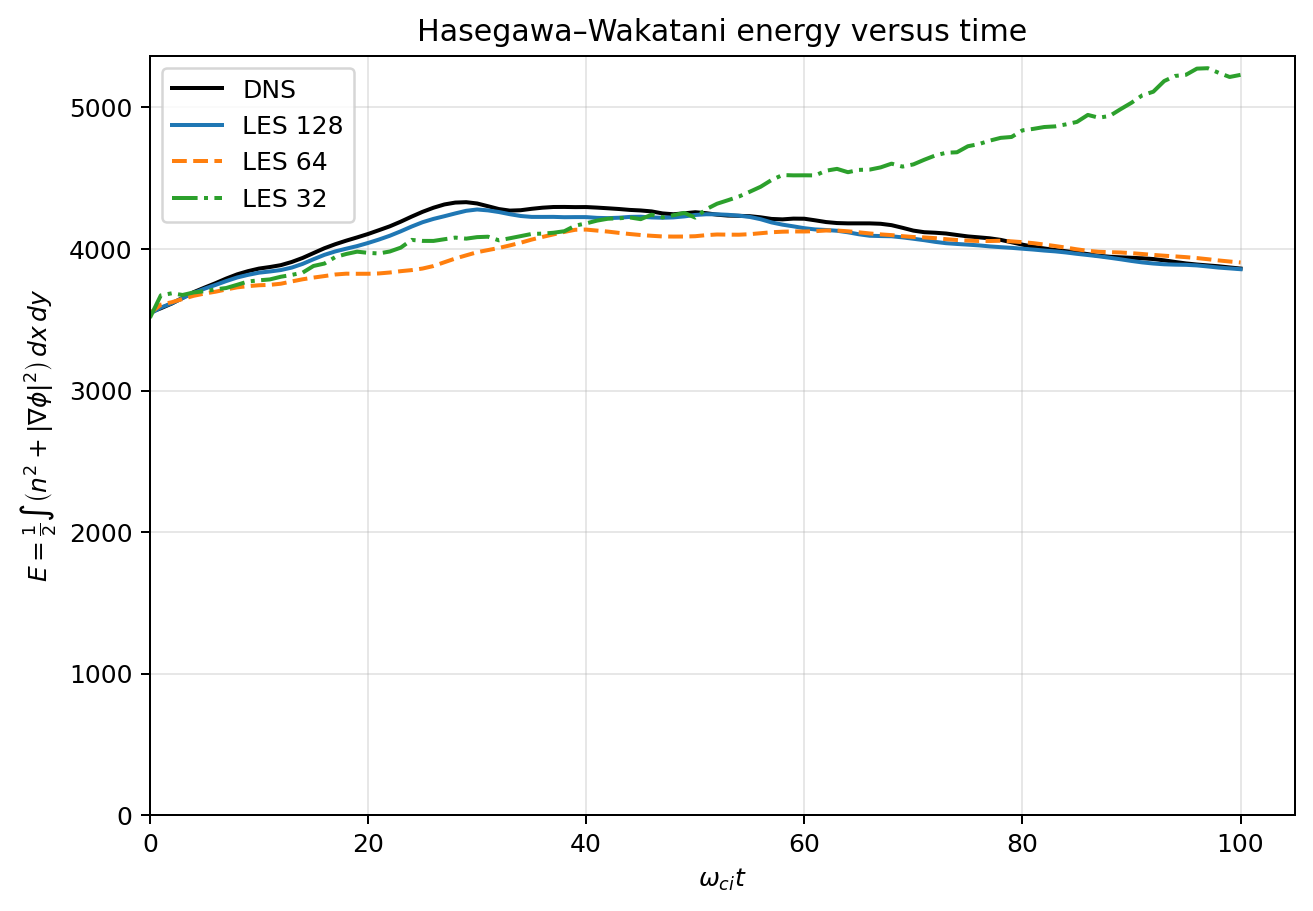
\includegraphics[width=\linewidth]{images/validation_current/mHW_N256/energy_vs_time.png}
\caption{mHW\_N256}
\end{subfigure}
\hfill
\begin{subfigure}[t]{0.48\textwidth}
\centering
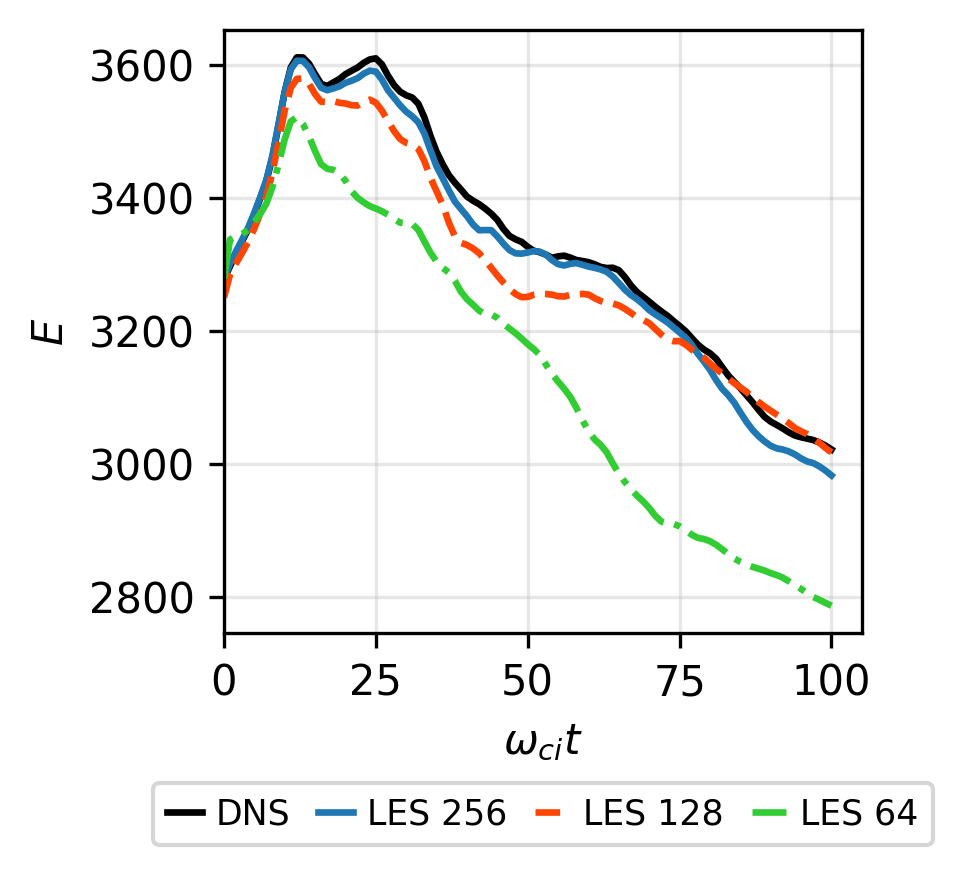
\includegraphics[width=\linewidth]{images/validation_current/mHW_N512/energy_vs_time.png}
\caption{mHW\_N512}
\end{subfigure}
\caption{Spatially integrated HW energy over $0\leq t\leq1000$ for HW and $0\leq t\leq100$ for mHW. Each available panel includes DNS and all three LES resolutions; energy uses cell-area quadrature on the diagnostic grid.}
\label{fig:energy}
\end{figure}

\begin{figure}[p]
\centering
\begin{subfigure}[t]{0.48\textwidth}
\centering
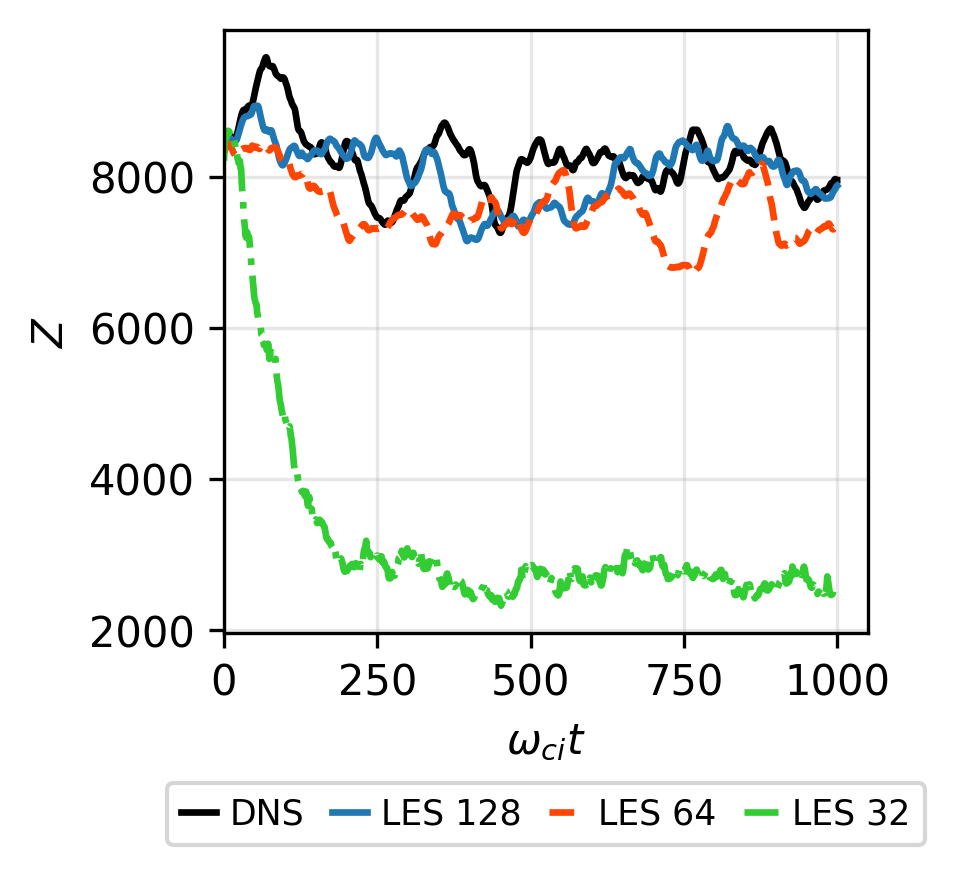
\includegraphics[width=\linewidth]{images/validation_current/HW_N256/enstrophy_vs_time.png}
\caption{HW\_N256}
\end{subfigure}
\hfill
\begin{subfigure}[t]{0.48\textwidth}
\centering
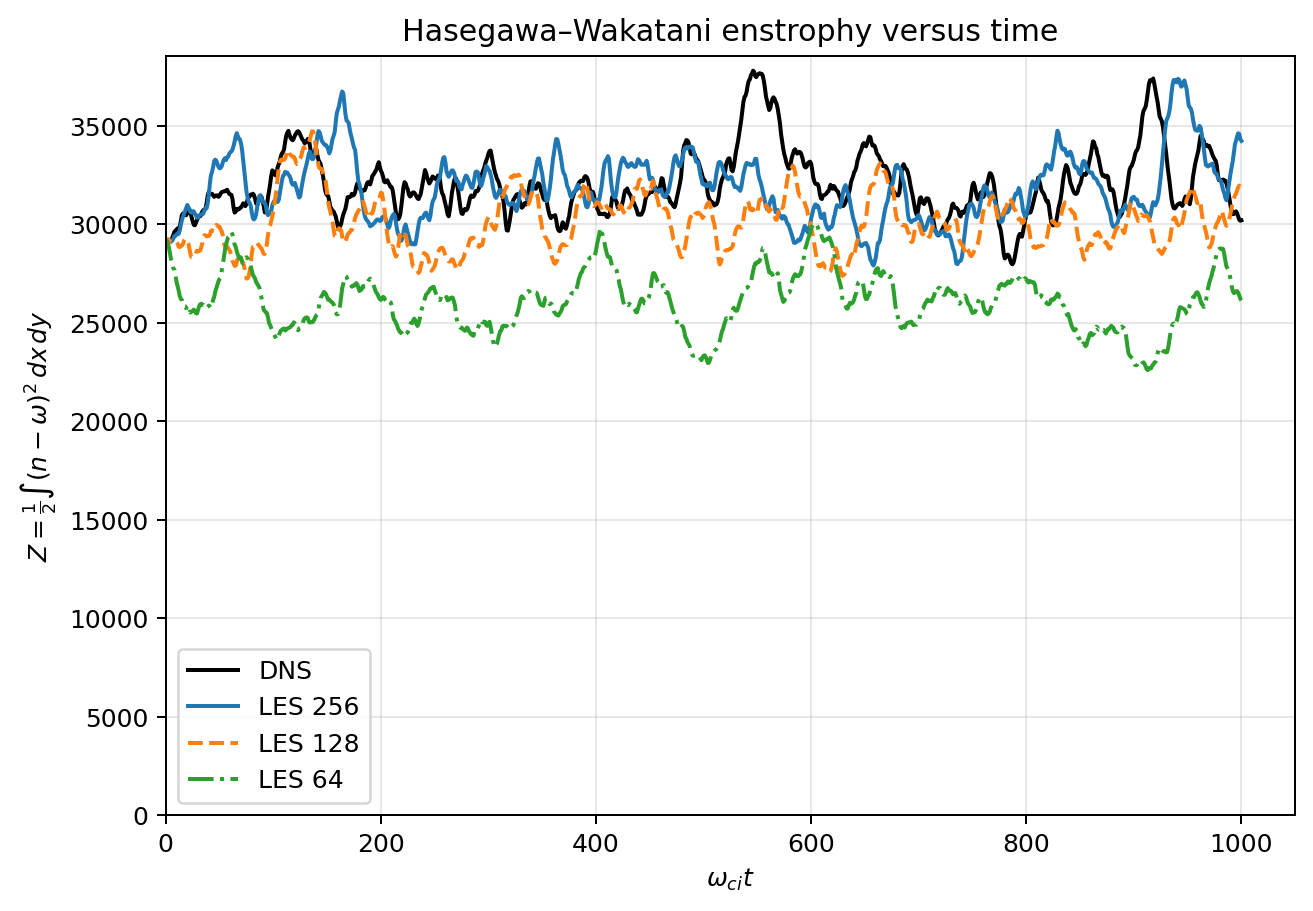
\includegraphics[width=\linewidth]{images/validation_current/HW_N512/enstrophy_vs_time.png}
\caption{HW\_N512}
\end{subfigure}
\par\smallskip
\begin{subfigure}[t]{0.48\textwidth}
\centering
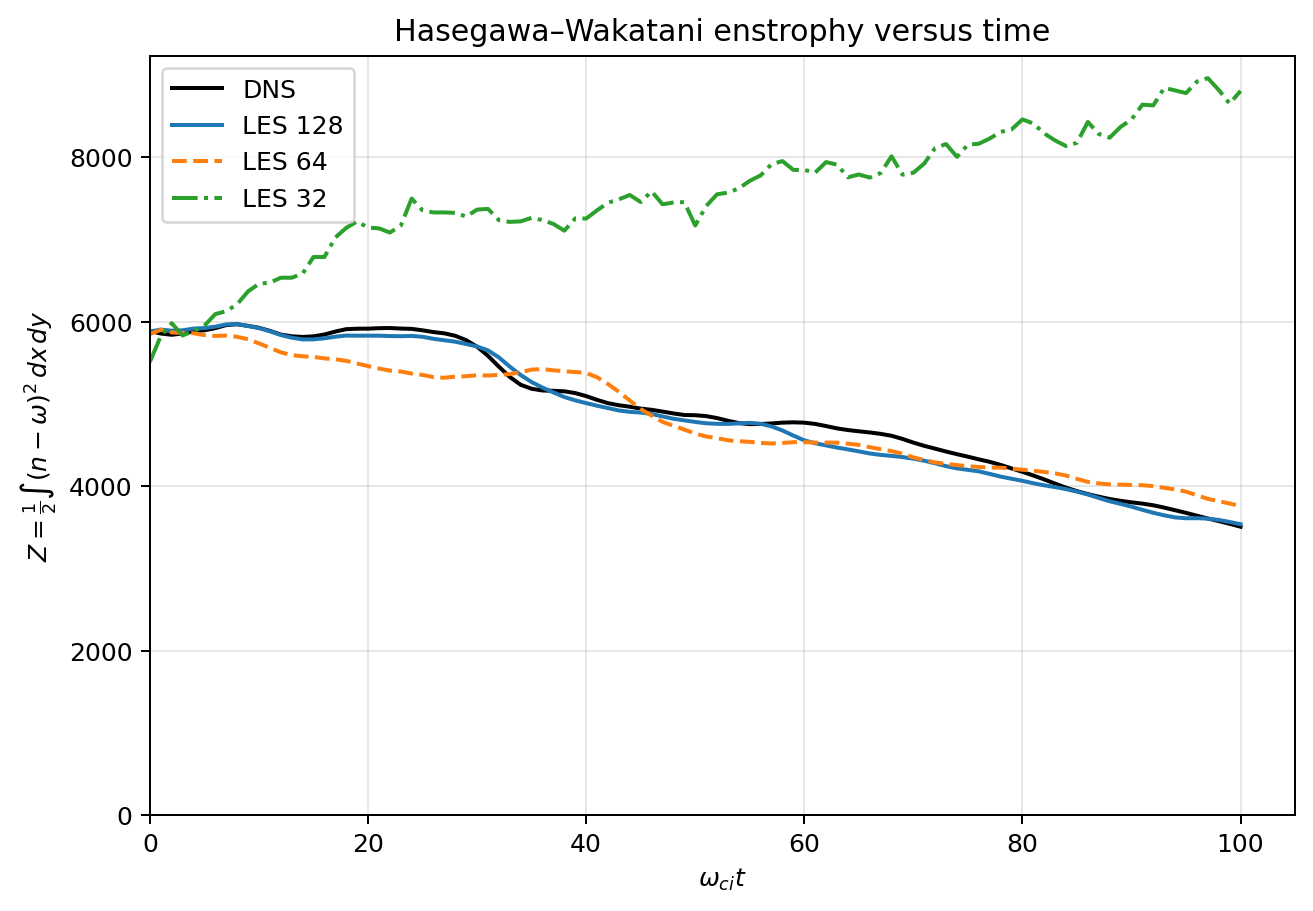
\includegraphics[width=\linewidth]{images/validation_current/mHW_N256/enstrophy_vs_time.png}
\caption{mHW\_N256}
\end{subfigure}
\hfill
\begin{subfigure}[t]{0.48\textwidth}
\centering
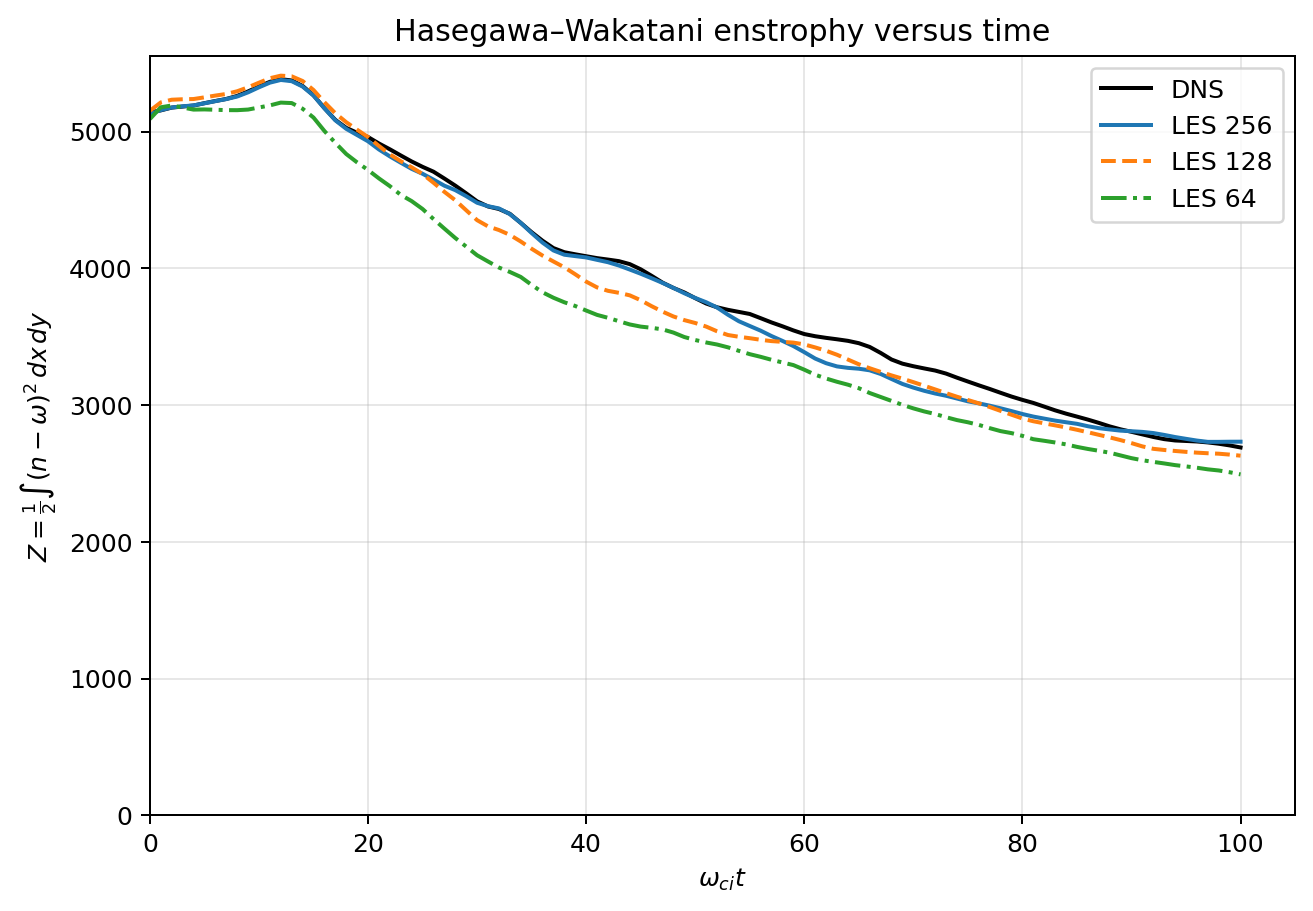
\includegraphics[width=\linewidth]{images/validation_current/mHW_N512/enstrophy_vs_time.png}
\caption{mHW\_N512}
\end{subfigure}
\caption{Generalized enstrophy over $0\leq t\leq1000$ for HW and $0\leq t\leq100$ for mHW. The coarse HW reconstructions have reduced enstrophy; the $32^2$ mHW\_N256 reconstruction instead develops excess enstrophy, while mHW\_N512 shows decay after an initial peak.}
\label{fig:enstrophy}
\end{figure}

\subsection{Spectral statistics}

The radial shell spectra include density and potential-gradient energy,
\begin{equation}
 E(k_s)=\frac12\sum_{\mathbf{k}\in\mathcal{S}_s}
 \left(|\widehat n_{\mathbf{k}}|^2+|\mathbf{k}|^2|\widehat\phi_{\mathbf{k}}|^2\right),
\end{equation}
where Fourier coefficients are normalized by the number of grid points and $\mathcal{S}_s$ is a radial wavenumber shell. This is a spectral energy density convention; summing the unsmoothed shells gives energy per unit area with spectral derivatives, rather than the finite-difference spatial integral above.

Figure~\ref{fig:spectra} compares the initial and final spectra. Initial spectra nearly overlap across the energetic modes. At $t=1000$, HW\_N256 with a $32^2$ LES mesh has a pronounced deficit across low and intermediate wavenumbers, consistent with its reduced integrated energy. A weak high-wavenumber tail remains, but does not compensate for the loss of energetic scales. The $128^2$ and $64^2$ LES spectra retain the main peak and broad decay more closely. HW\_N512 preserves the broad spectral shape across all three LES meshes, with differences at low wavenumbers, around the peak and in the weak dissipative tail. At $t=100$, the mHW\_N512 spectra remain close through the principal energy-containing range, with smaller differences toward the tail.

For mHW\_N256, the two finer LES meshes retain the final DNS spectral shape closely. The $32^2$ reconstruction has excess energy at intermediate and high wavenumbers, particularly for $k\gtrsim1$, consistent with its growing generalized enstrophy. Agreement near the principal spectral peak therefore does not imply correct small-scale behaviour.

Spectral agreement on logarithmic axes should be assessed together with the integrated diagnostics: similar shapes can coexist with energy deficits. The dotted line marks the $64^2$-grid Nyquist wavenumber in all panels; it is a fixed reference, not the cutoff of every LES mesh or a measured accuracy threshold.

\begin{figure}[p]
\centering
\begin{subfigure}[t]{0.98\textwidth}
\centering
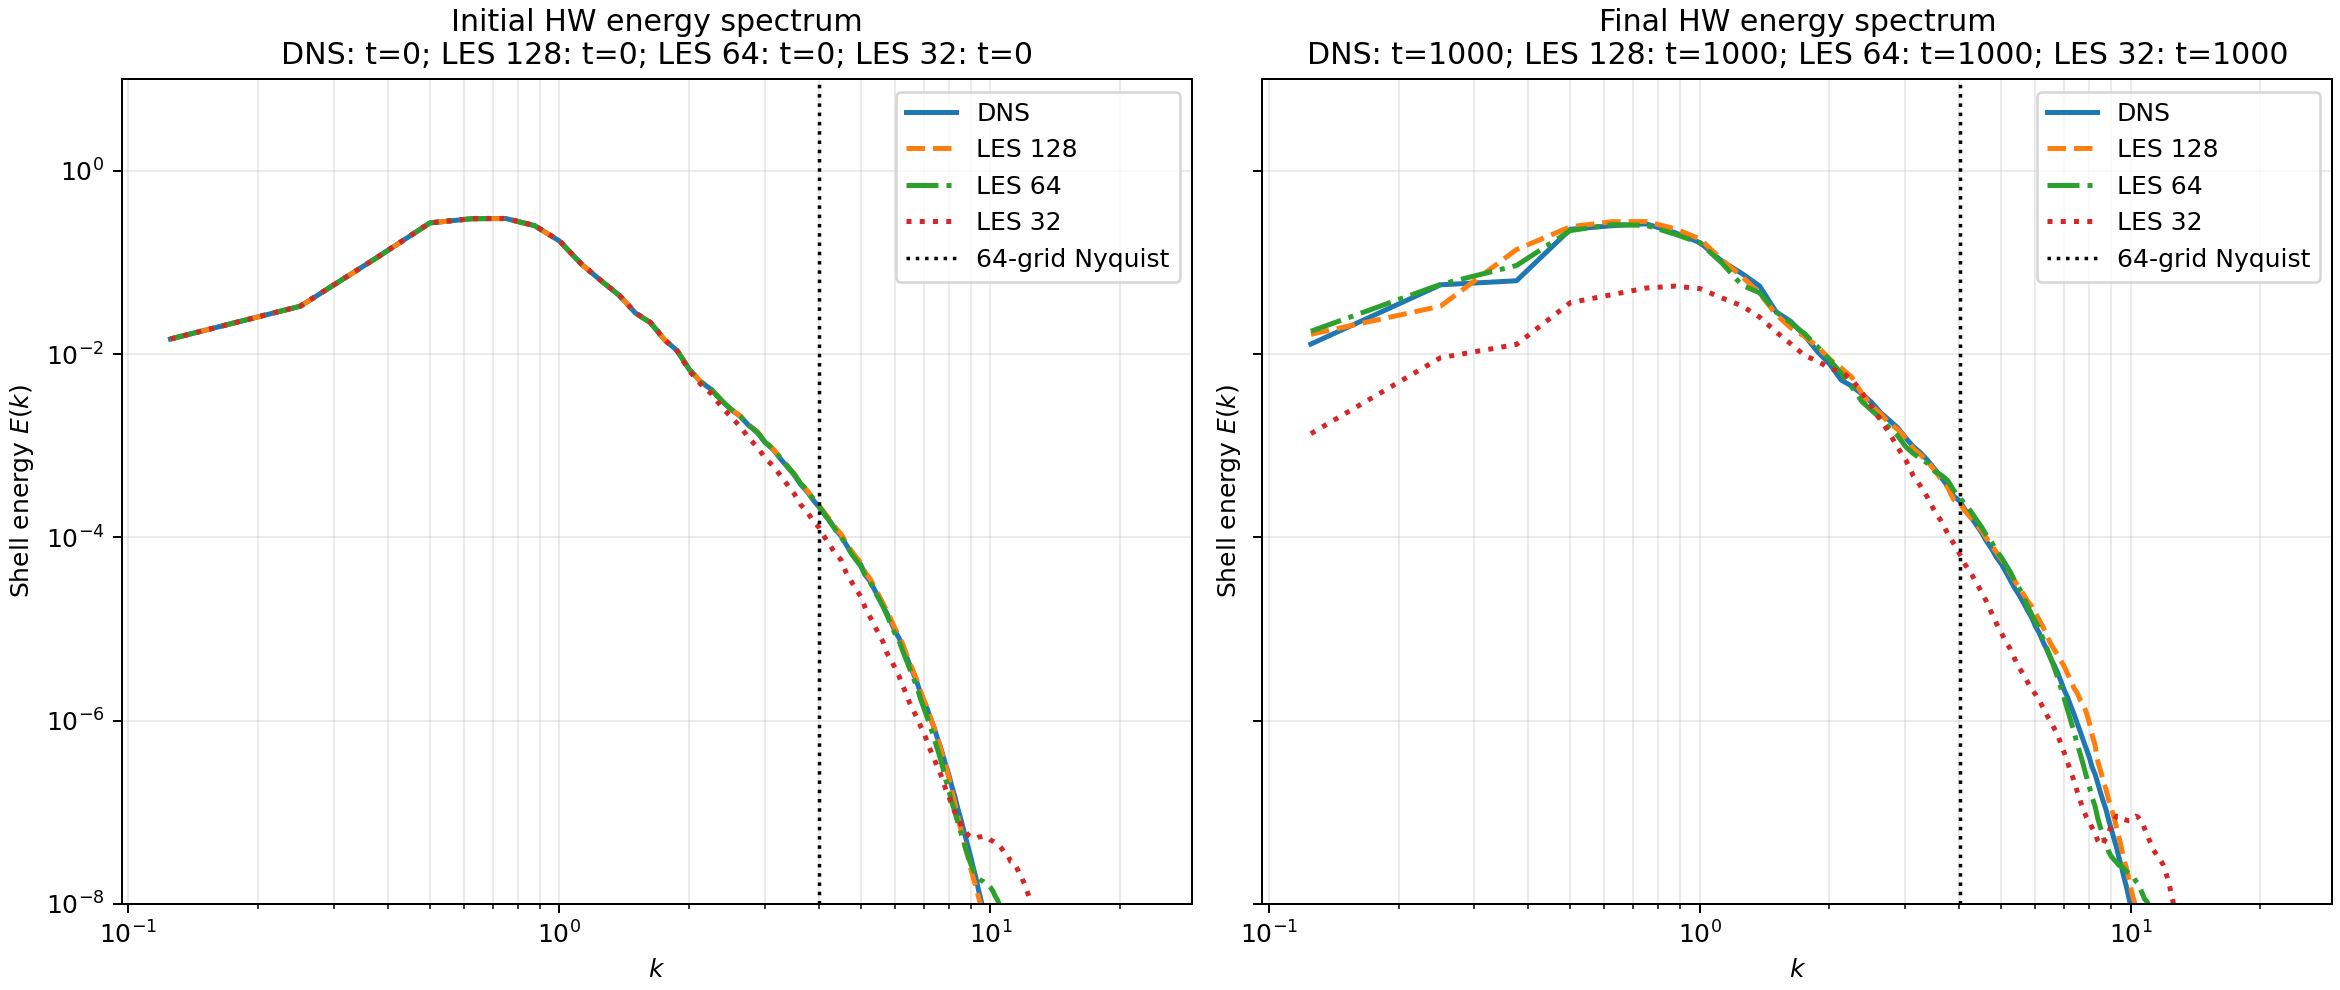
\includegraphics[width=\linewidth,height=0.175\textheight,keepaspectratio]{images/validation_current/HW_N256/hw_energy_spectra_initial_final.png}
\caption{HW\_N256}
\end{subfigure}
\par\smallskip
\begin{subfigure}[t]{0.98\textwidth}
\centering
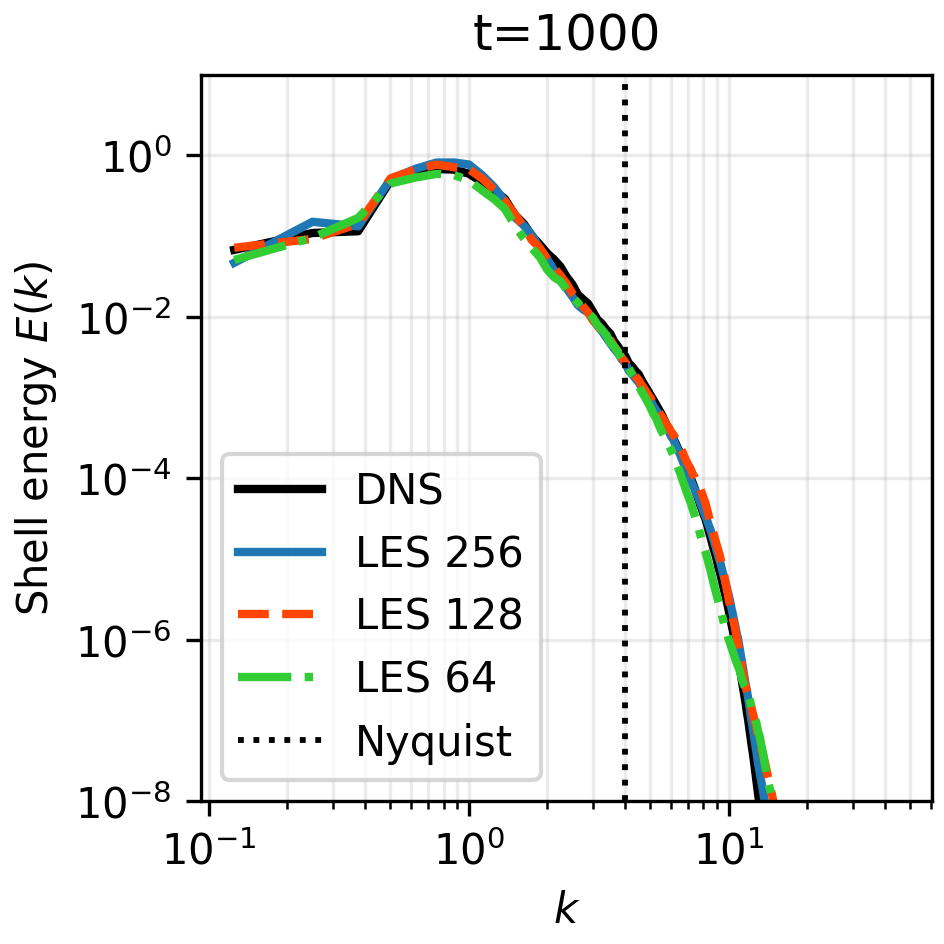
\includegraphics[width=\linewidth,height=0.175\textheight,keepaspectratio]{images/validation_current/HW_N512/hw_energy_spectra_initial_final.png}
\caption{HW\_N512}
\end{subfigure}
\par\smallskip
\begin{subfigure}[t]{0.98\textwidth}
\centering
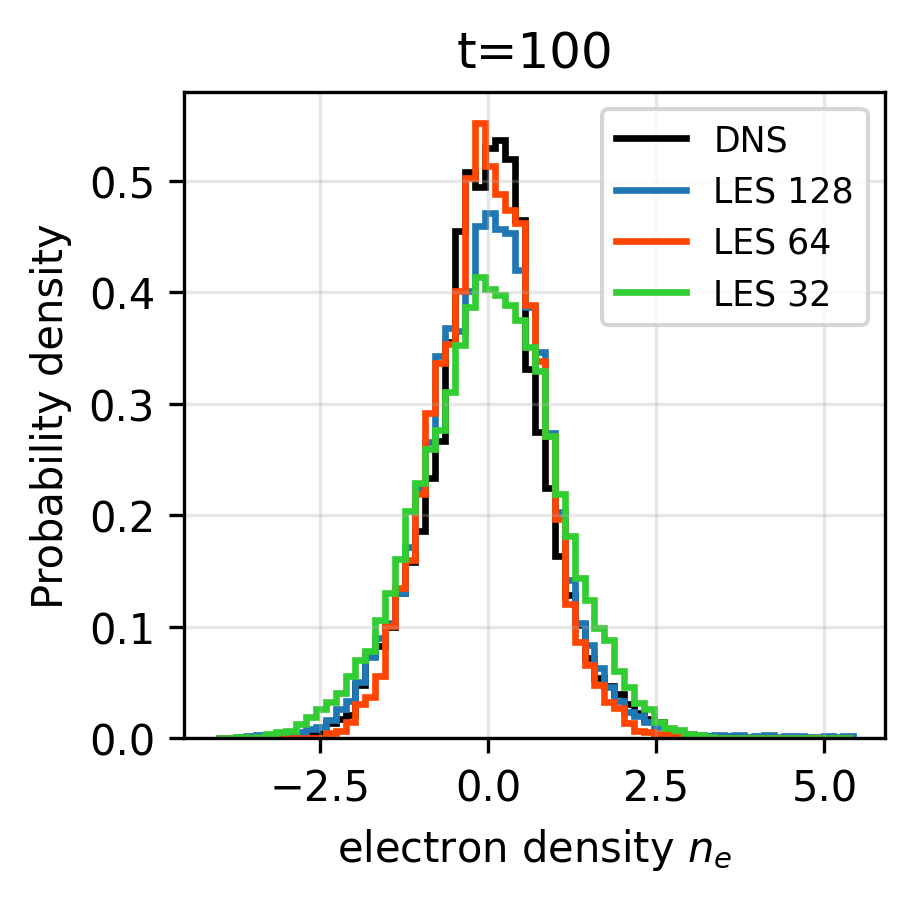
\includegraphics[width=\linewidth,height=0.175\textheight,keepaspectratio]{images/validation_current/mHW_N256/U_pdf_vs_time.png}
\caption{mHW\_N256}
\end{subfigure}
\par\smallskip
\begin{subfigure}[t]{0.98\textwidth}
\centering
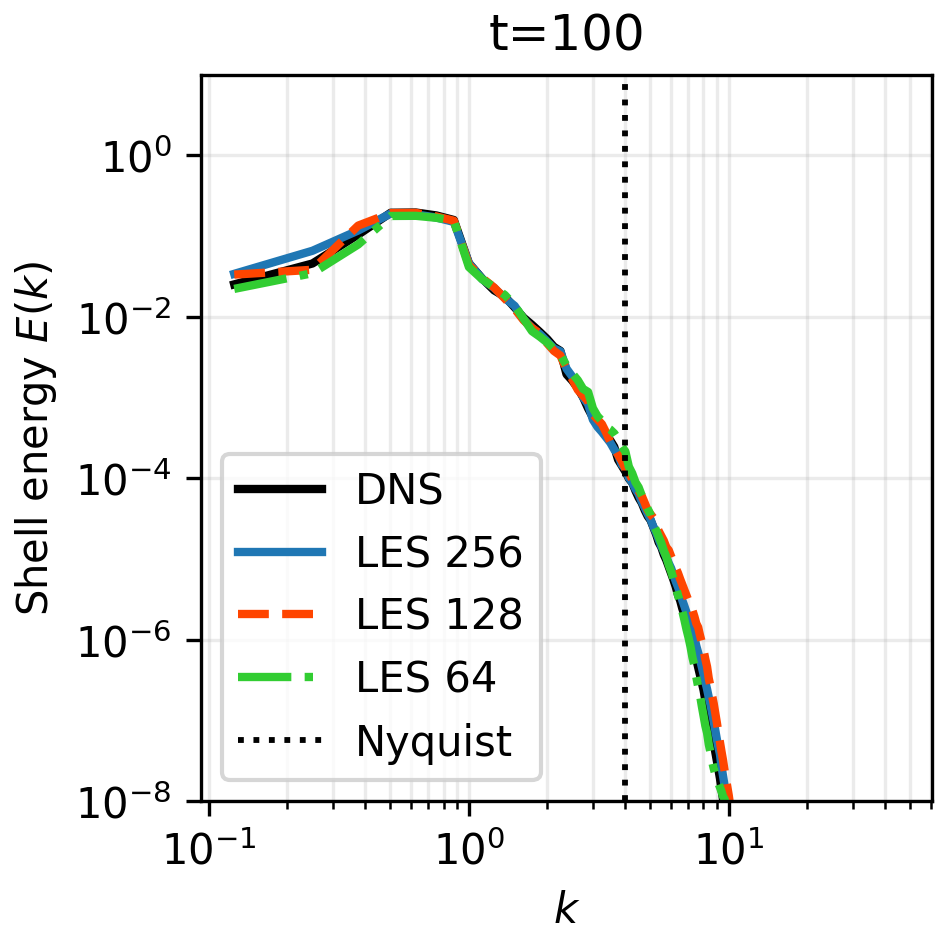
\includegraphics[width=\linewidth,height=0.175\textheight,keepaspectratio]{images/validation_current/mHW_N512/hw_energy_spectra_initial_final.png}
\caption{mHW\_N512}
\end{subfigure}
\caption{Initial ($t=0$, left) and final ($t=1000$ for HW and $t=100$ for mHW, right) shell-summed HW energy spectra for the available cases and all three LES resolutions. The dotted vertical line marks the $64^2$-grid Nyquist wavenumber.}
\label{fig:spectra}
\end{figure}

\subsection{Probability-density functions}

Figures~\ref{fig:pdf-density}--\ref{fig:pdf-vorticity} compare spatial PDFs at the two endpoints. The stored channels $U$, $V$ and $P$ denote $n$, $\phi$ and $\zeta$, respectively. Despite their filenames, these are endpoint distributions rather than PDFs accumulated over time.

Initial PDFs nearly overlap for all resolutions. At $t=1000$, the HW\_N256 $32^2$ LES has much narrower density and potential distributions: their central PDF peaks reach approximately $0.6$, compared with about $0.28$ for DNS. The vorticity PDF also becomes more sharply peaked. These changes agree with the loss of field amplitude indicated by energy and enstrophy. The two finer LES meshes retain broader distributions closer to DNS. For HW\_N512, the final distributions remain broadly similar, although the coarsest mesh sharpens the central vorticity peak and changes the density and potential peaks.

At $t=100$, mHW\_N512 retains a single dominant density peak, a broad structured potential PDF and a two-peaked vorticity PDF. The LES curves reproduce these qualitative shapes. Coarser density reconstructions have higher central peaks, while the potential and vorticity distributions differ locally around their peaks and the intervening troughs. Agreement of these spatial distributions does not imply that the instantaneous fields remain phase-aligned.

In mHW\_N256, the $128^2$ and $64^2$ reconstructions retain the final density and vorticity PDFs more closely than $32^2$. At $t=100$, the coarsest density PDF has a lower central peak (about $0.37$ versus $0.53$ for DNS) and broader tails; its vorticity PDF likewise broadens, with a peak near $0.26$ versus $0.39$ for DNS. The potential PDF remains broad and structured, with local differences between all reconstructions and DNS. These changes support the energy and enstrophy evidence of excessive fluctuations on the coarsest mesh.

These one-point statistics complement the field comparisons but do not measure spatial phase agreement or density--potential correlations. Their agreement can therefore coexist with differences in transport. The displayed linear-scale PDFs also do not establish quantitative accuracy for rare-event tails.

\begin{figure}[p]
\centering
\begin{subfigure}[t]{0.98\textwidth}
\centering
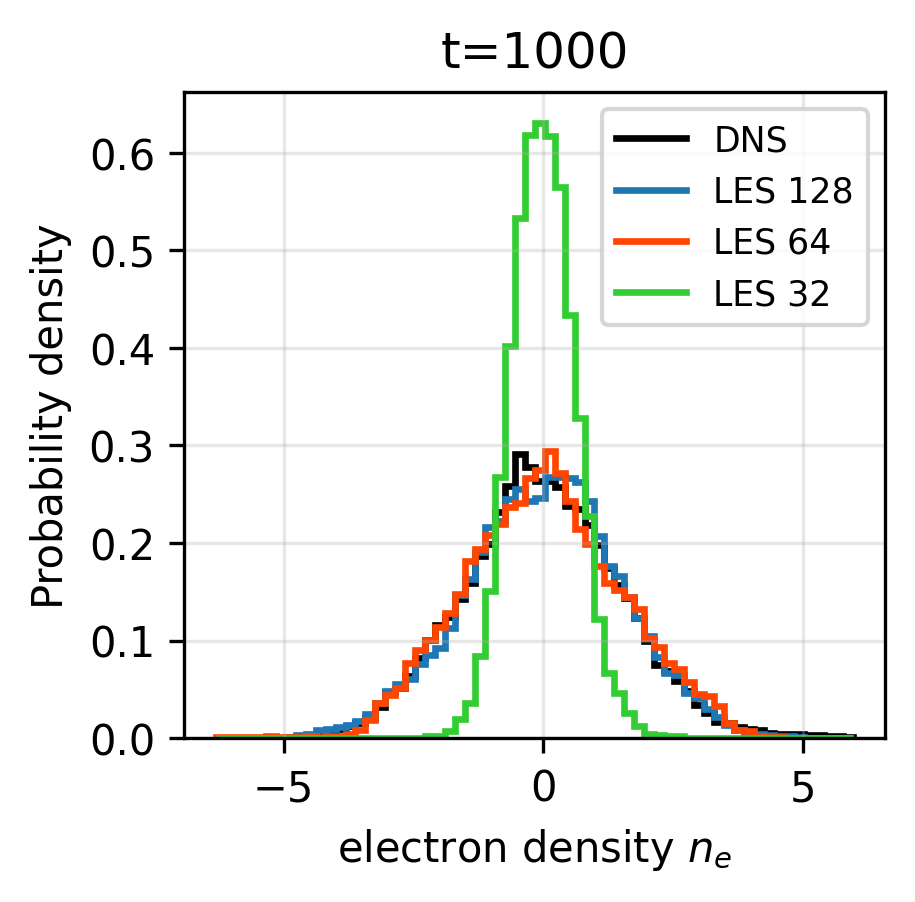
\includegraphics[width=\linewidth,height=0.175\textheight,keepaspectratio]{images/validation_current/HW_N256/U_pdf_vs_time.png}
\caption{HW\_N256}
\end{subfigure}
\par\smallskip
\begin{subfigure}[t]{0.98\textwidth}
\centering
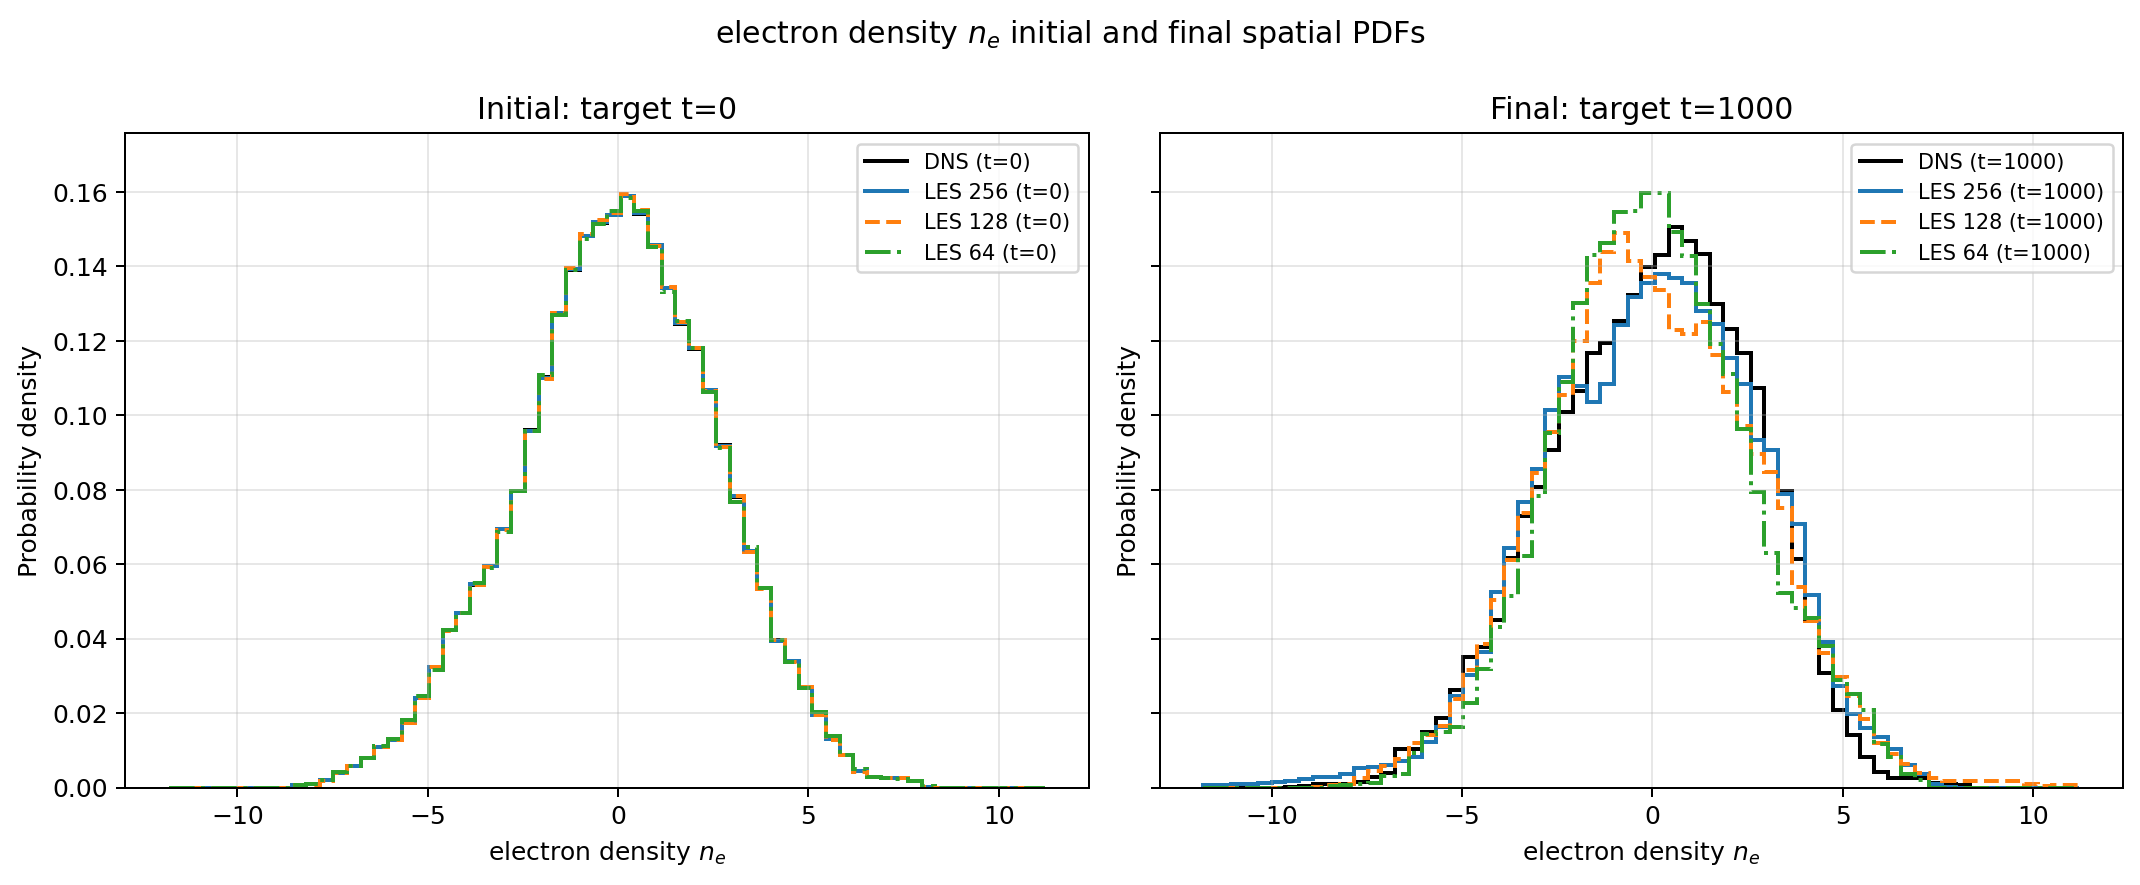
\includegraphics[width=\linewidth,height=0.175\textheight,keepaspectratio]{images/validation_current/HW_N512/U_pdf_vs_time.png}
\caption{HW\_N512}
\end{subfigure}
\par\smallskip
\begin{subfigure}[t]{0.98\textwidth}
\centering
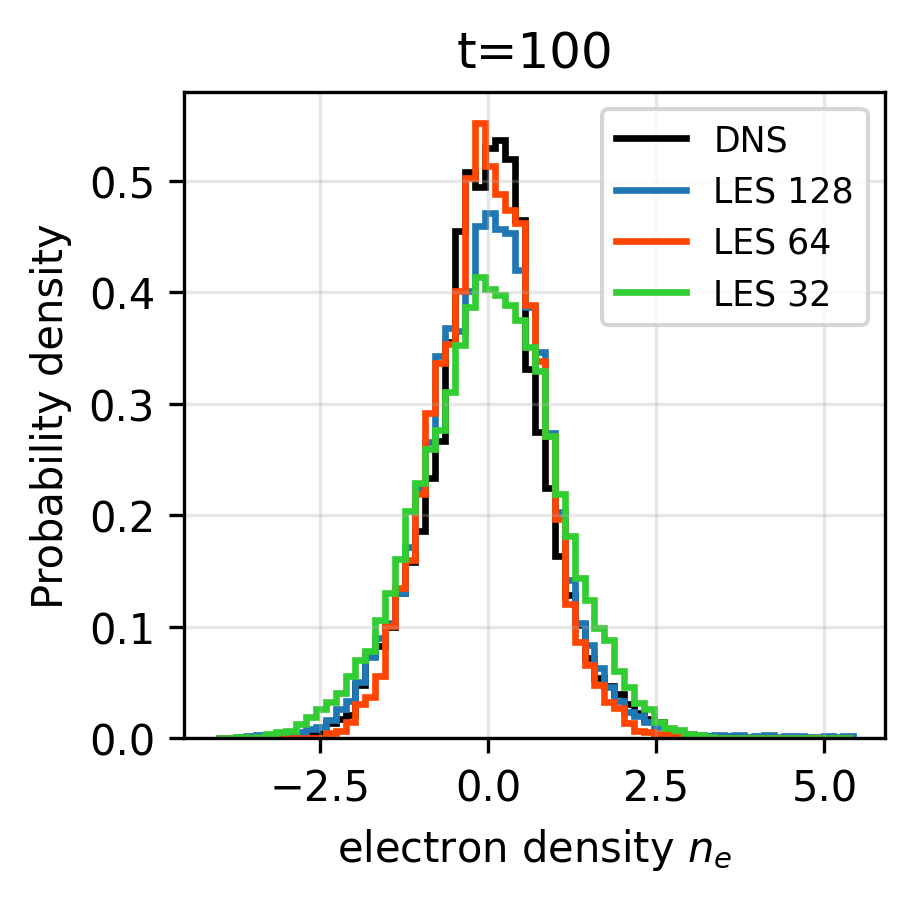
\includegraphics[width=\linewidth,height=0.175\textheight,keepaspectratio]{images/validation_current/mHW_N256/U_pdf_vs_time.png}
\caption{mHW\_N256}
\end{subfigure}
\par\smallskip
\begin{subfigure}[t]{0.98\textwidth}
\centering
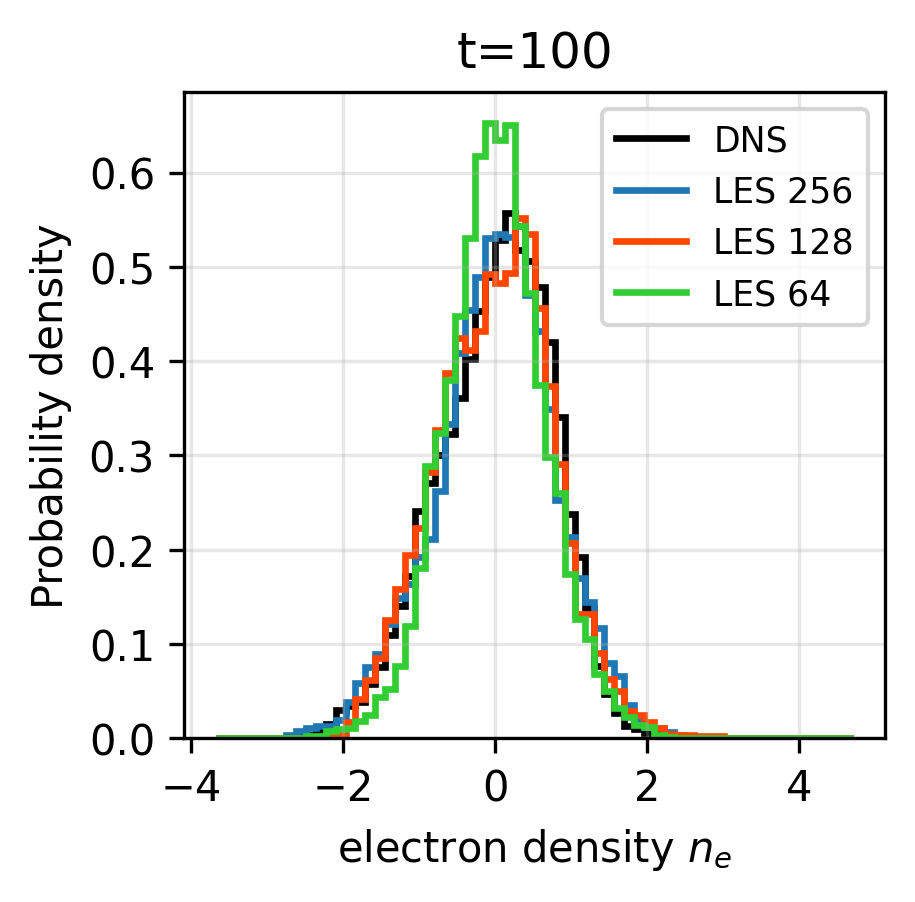
\includegraphics[width=\linewidth,height=0.175\textheight,keepaspectratio]{images/validation_current/mHW_N512/U_pdf_vs_time.png}
\caption{mHW\_N512}
\end{subfigure}
\caption{Spatial PDFs of density $n$ at $t=0$ (left) and $t=1000$ for HW or $t=100$ for mHW (right). Each available case includes DNS and three LES resolutions.}
\label{fig:pdf-density}
\end{figure}

\begin{figure}[p]
\centering
\begin{subfigure}[t]{0.98\textwidth}
\centering
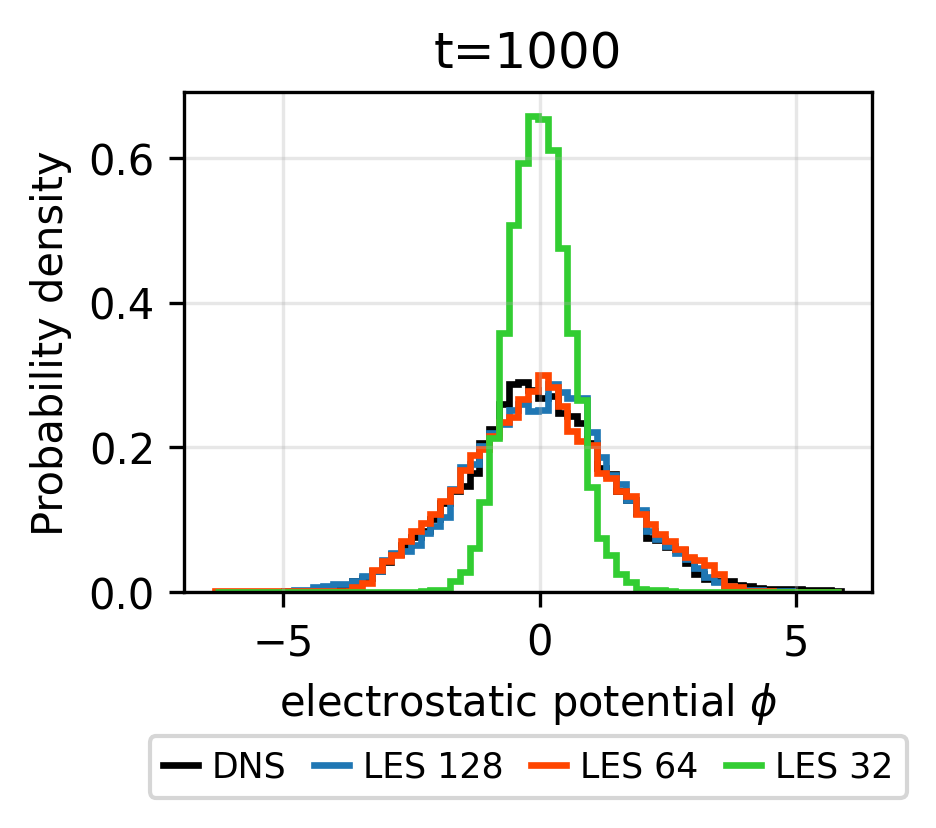
\includegraphics[width=\linewidth,height=0.175\textheight,keepaspectratio]{images/validation_current/HW_N256/V_pdf_vs_time.png}
\caption{HW\_N256}
\end{subfigure}
\par\smallskip
\begin{subfigure}[t]{0.98\textwidth}
\centering
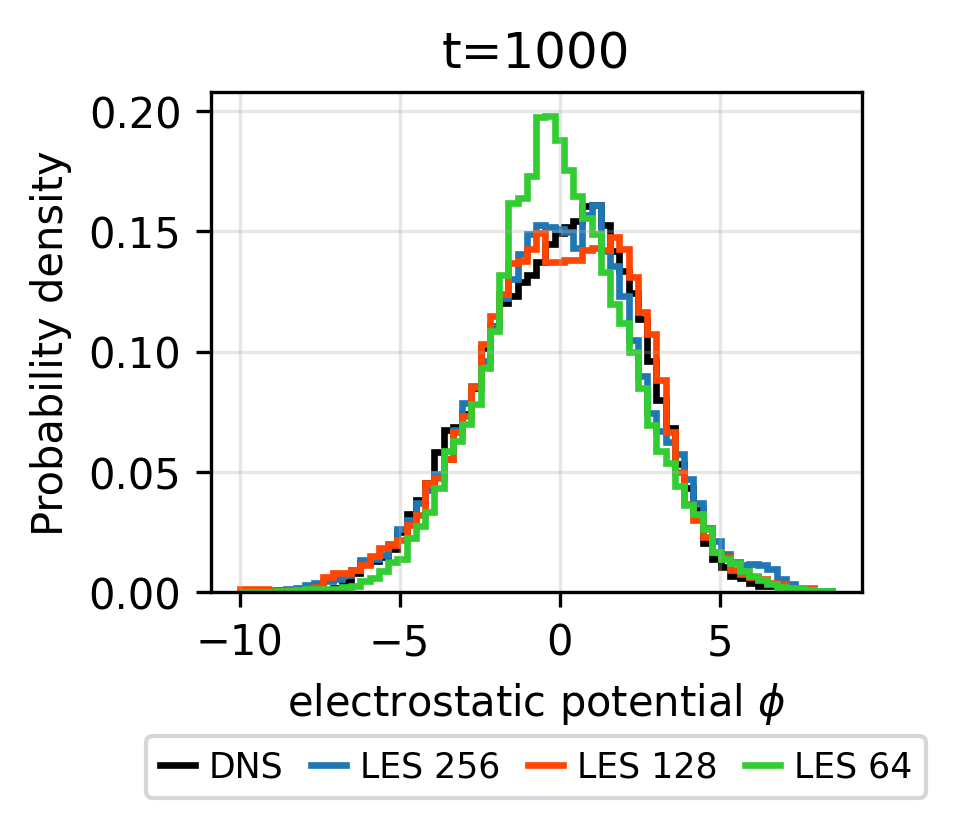
\includegraphics[width=\linewidth,height=0.175\textheight,keepaspectratio]{images/validation_current/HW_N512/V_pdf_vs_time.png}
\caption{HW\_N512}
\end{subfigure}
\par\smallskip
\begin{subfigure}[t]{0.98\textwidth}
\centering
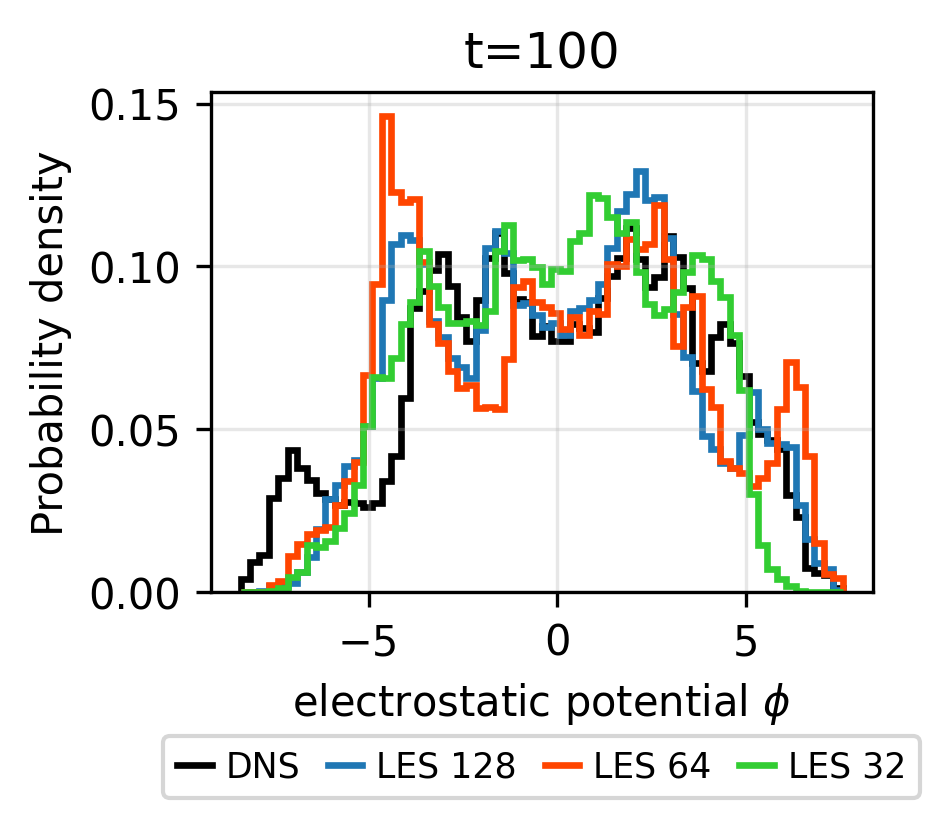
\includegraphics[width=\linewidth,height=0.175\textheight,keepaspectratio]{images/validation_current/mHW_N256/V_pdf_vs_time.png}
\caption{mHW\_N256}
\end{subfigure}
\par\smallskip
\begin{subfigure}[t]{0.98\textwidth}
\centering
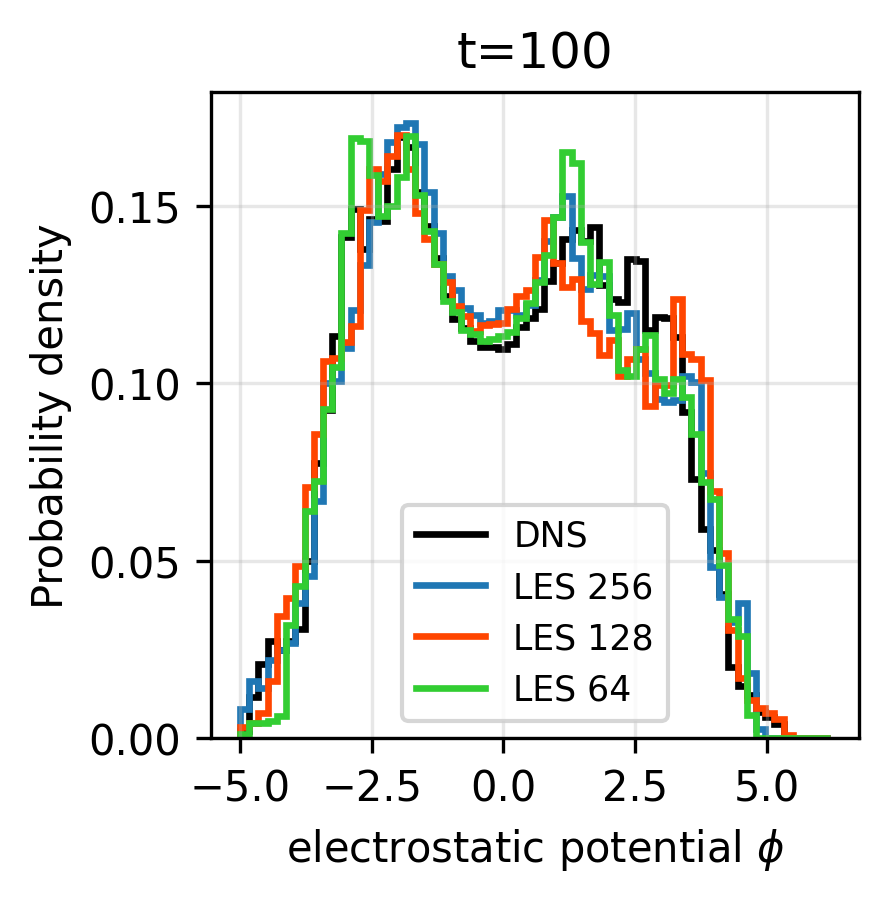
\includegraphics[width=\linewidth,height=0.175\textheight,keepaspectratio]{images/validation_current/mHW_N512/V_pdf_vs_time.png}
\caption{mHW\_N512}
\end{subfigure}
\caption{Spatial PDFs of electrostatic potential $\phi$ at $t=0$ (left) and $t=1000$ for HW or $t=100$ for mHW (right). Each available case includes DNS and three LES resolutions.}
\label{fig:pdf-potential}
\end{figure}

\begin{figure}[p]
\centering
\begin{subfigure}[t]{0.98\textwidth}
\centering
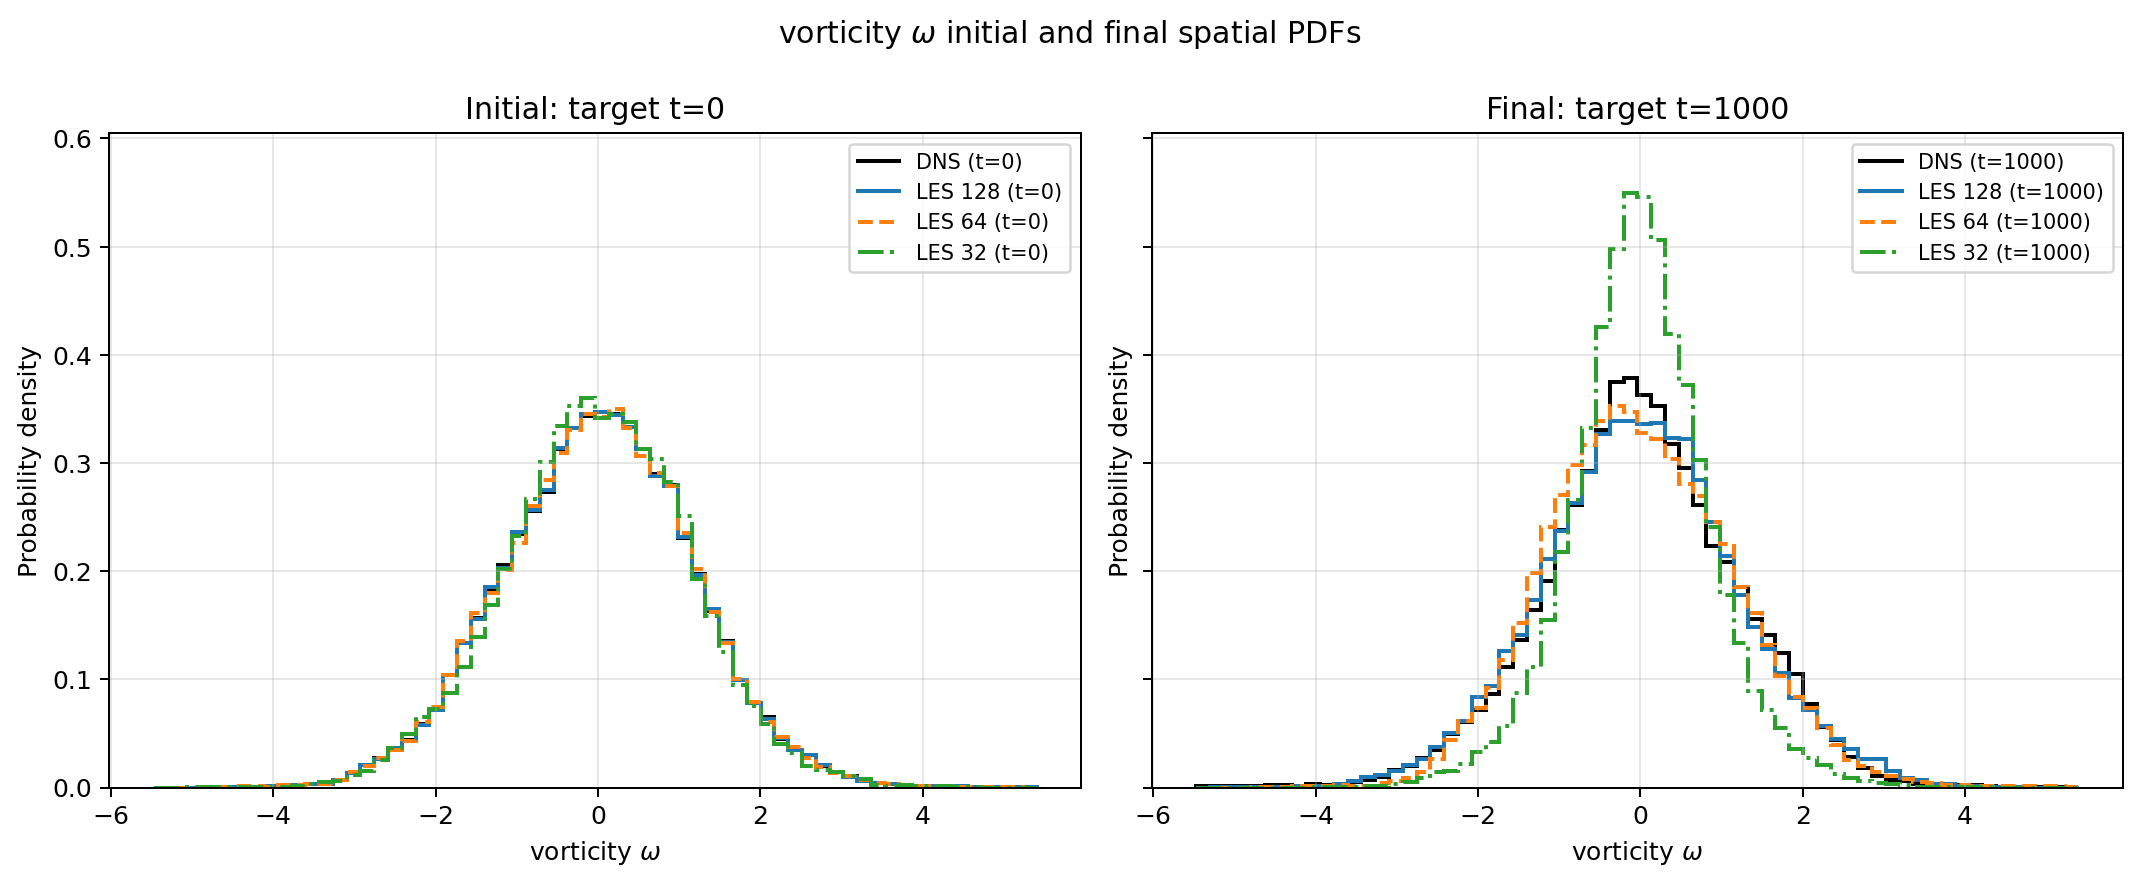
\includegraphics[width=\linewidth,height=0.175\textheight,keepaspectratio]{images/validation_current/HW_N256/P_pdf_vs_time.png}
\caption{HW\_N256}
\end{subfigure}
\par\smallskip
\begin{subfigure}[t]{0.98\textwidth}
\centering
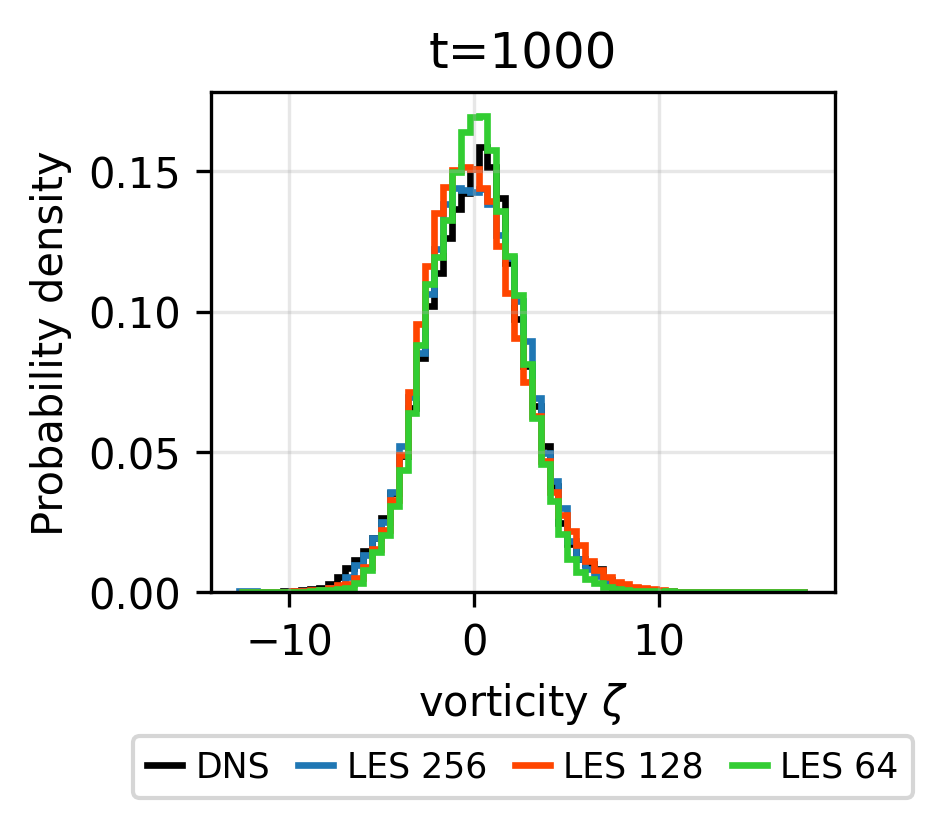
\includegraphics[width=\linewidth,height=0.175\textheight,keepaspectratio]{images/validation_current/HW_N512/P_pdf_vs_time.png}
\caption{HW\_N512}
\end{subfigure}
\par\smallskip
\begin{subfigure}[t]{0.98\textwidth}
\centering
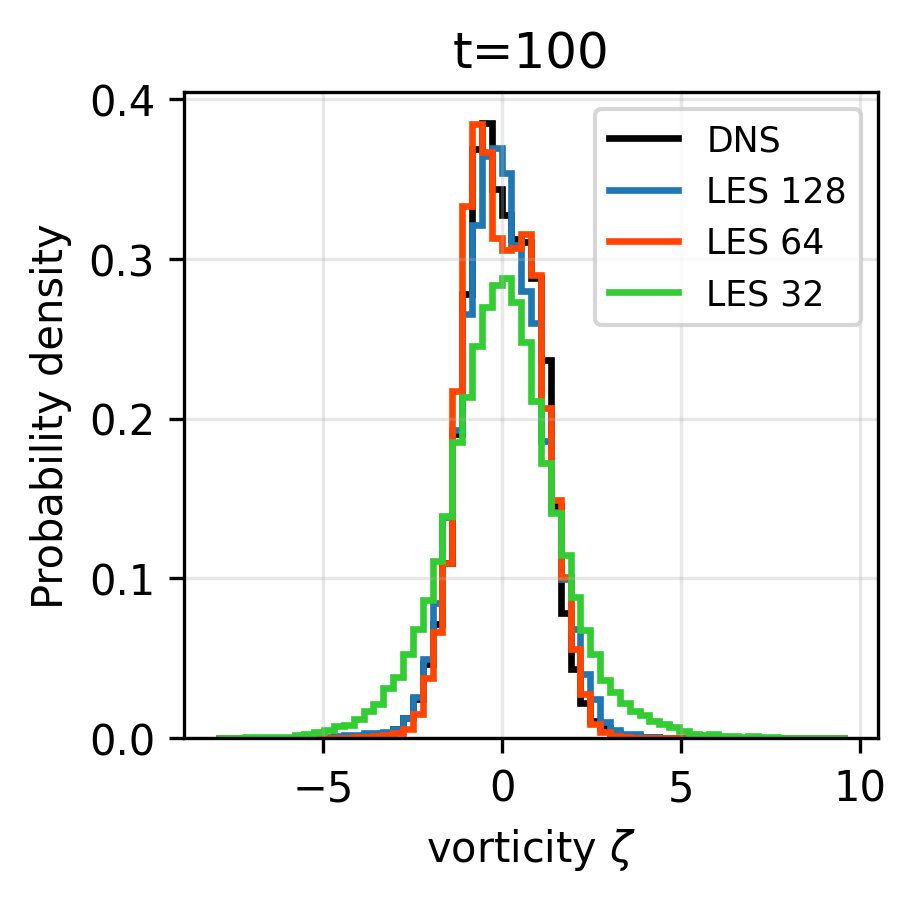
\includegraphics[width=\linewidth,height=0.175\textheight,keepaspectratio]{images/validation_current/mHW_N256/P_pdf_vs_time.png}
\caption{mHW\_N256}
\end{subfigure}
\par\smallskip
\begin{subfigure}[t]{0.98\textwidth}
\centering
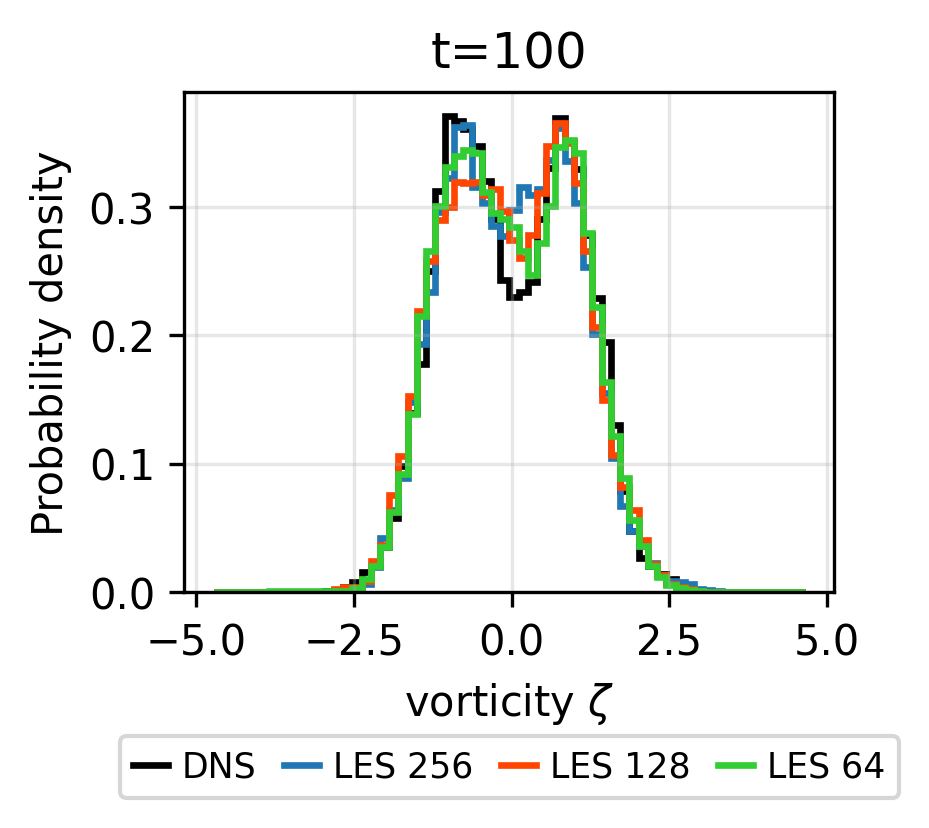
\includegraphics[width=\linewidth,height=0.175\textheight,keepaspectratio]{images/validation_current/mHW_N512/P_pdf_vs_time.png}
\caption{mHW\_N512}
\end{subfigure}
\caption{Spatial PDFs of vorticity $\zeta$ (labelled $\omega$ in the plots) at $t=0$ (left) and $t=1000$ for HW or $t=100$ for mHW (right). Each available case includes DNS and three LES resolutions.}
\label{fig:pdf-vorticity}
\end{figure}

\subsection{Transport diagnostics}

The flux diagnostic removes the poloidal mean density, $n'=n-\langle n\rangle_y$, and uses $v_x=-\partial_y\phi$ and $v_y=\partial_x\phi$. The displayed domain averages are
\begin{equation}
 \overline\Gamma_x=-\langle n'\partial_y\phi\rangle_{x,y},\qquad
 \overline\Gamma_y=\langle n'\partial_x\phi\rangle_{x,y}.
\end{equation}
The same fourth-order periodic derivatives used for energy enter the flux calculation. A zonal velocity contributes no net flux to this diagnostic because the poloidal mean of $n'$ vanishes.

Figure~\ref{fig:particle-flux} shows positive radial transport in all available cases. For HW\_N256, DNS fluctuates mainly around $0.11$--$0.15$, while the $32^2$ LES drops to approximately $0.04$ after the initial transient. The $128^2$ and $64^2$ meshes retain substantially more radial transport, although the latter is generally below DNS. In HW\_N512, DNS and the finest LES fluctuate mostly around $0.7$--$0.9$, whereas the coarsest mesh is typically around $0.55$--$0.65$. These deficits accompany the lower energy and enstrophy of the coarse solutions.

For mHW\_N256, DNS radial flux decreases from approximately $0.12$ to $0.026$ by $t=100$. The $128^2$ and $64^2$ reconstructions broadly follow this decline but end higher, at approximately $0.035$ and $0.033$. The $32^2$ reconstruction remains strongly fluctuating around $0.07$--$0.10$ after its initial transient and ends near $0.090$, more than three times the DNS value. Its excess transport accompanies the growth of energy and enstrophy rather than the DNS tendency toward laminarization. The finer meshes capture the early poloidal-flux extrema more closely; the coarsest mesh differs substantially in both timing and sign.

The mHW\_N512 radial flux peaks near $0.10$ early in the evolution and decreases to approximately $0.02$--$0.03$ by $t=100$. The finest LES follows the overall decline closely, and coarser meshes generally underpredict the early and intermediate transport. The marked decrease in transport accompanies the decay of generalized enstrophy as the flow evolves toward laminarization.

Poloidal transport fluctuates about zero and is smaller than radial transport. In HW\_N256, the $32^2$ LES strongly suppresses these fluctuations after the transient; the two finer meshes retain larger excursions but do not reproduce every DNS event. In HW\_N512, all curves remain strongly time dependent, with differences in the timing and amplitude of individual excursions. The mHW\_N512 LES curves capture the early negative excursions near $t\simeq13$ and $t\simeq27$ qualitatively, but differ from DNS later, including in sign. These comparisons distinguish preservation of the overall transport trend from agreement of instantaneous fluxes.

\begin{figure}[p]
\centering
\begin{subfigure}[t]{0.48\textwidth}
\centering
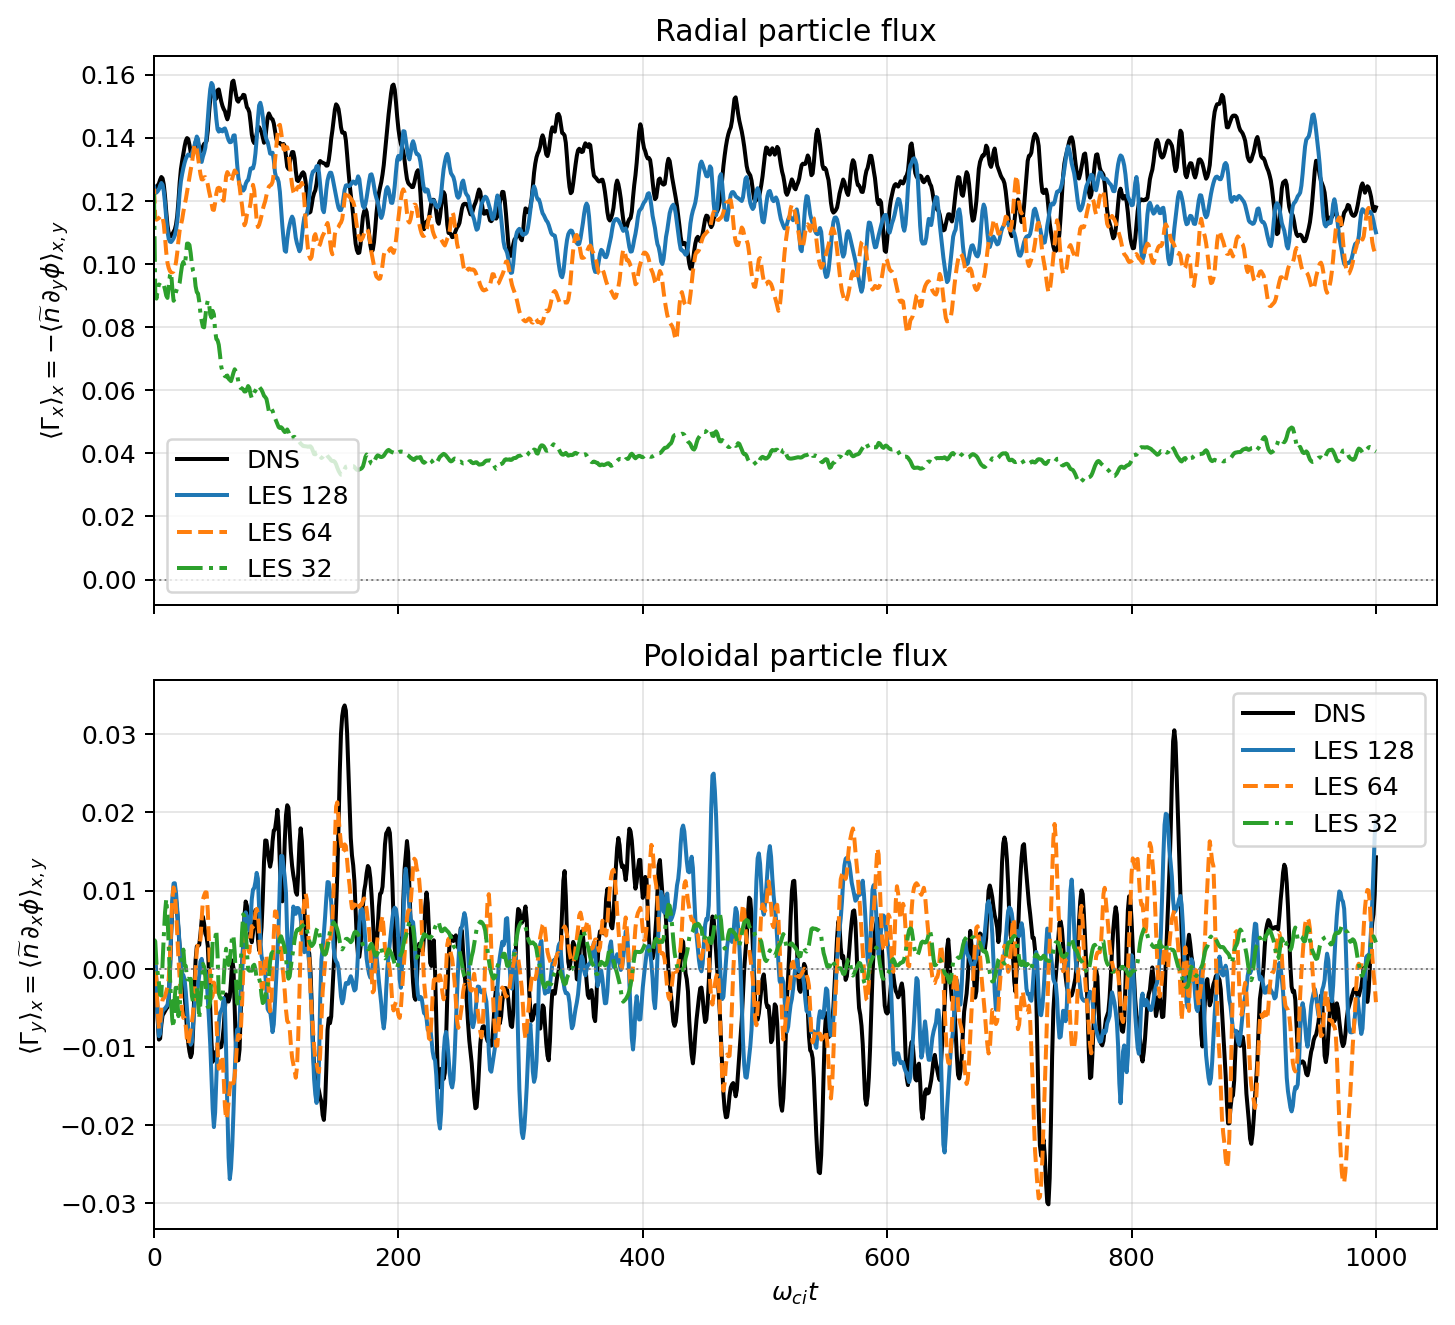
\includegraphics[width=\linewidth]{images/validation_current/HW_N256/particle_flux_vs_time.png}
\caption{HW\_N256}
\end{subfigure}
\hfill
\begin{subfigure}[t]{0.48\textwidth}
\centering
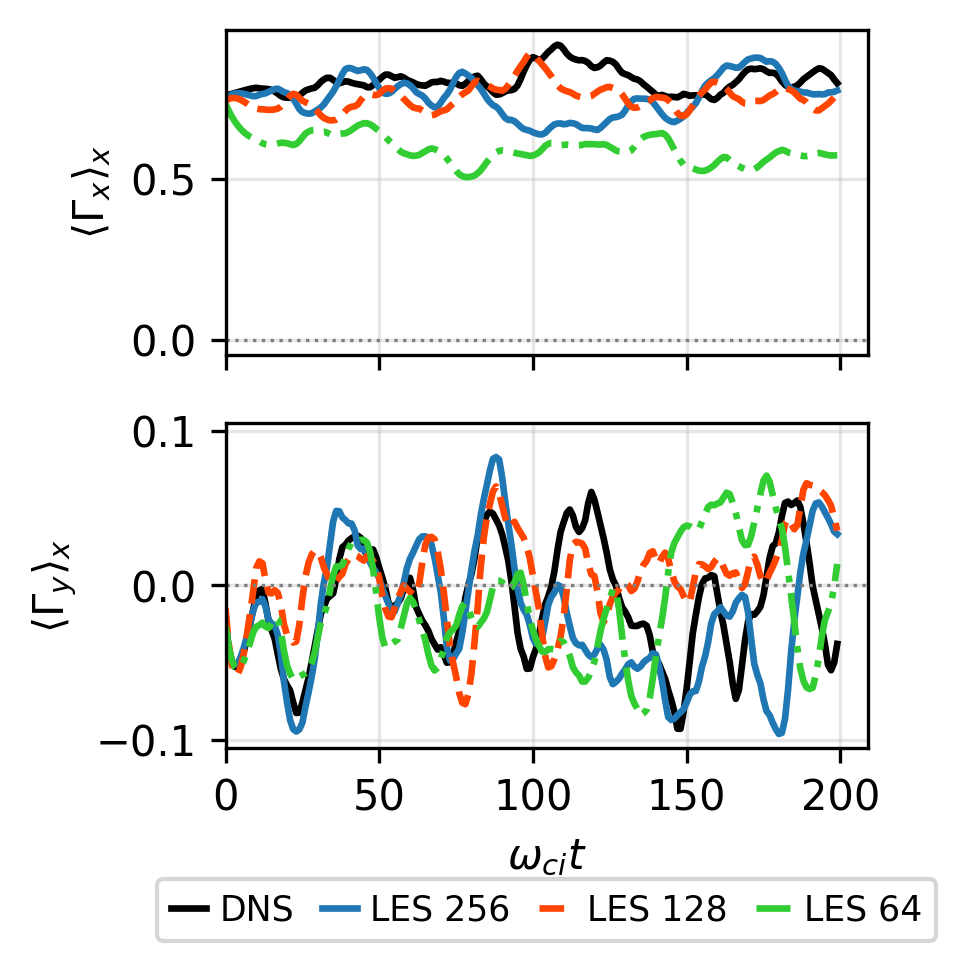
\includegraphics[width=\linewidth]{images/validation_current/HW_N512/particle_flux_vs_time.png}
\caption{HW\_N512}
\end{subfigure}
\par\smallskip
\begin{subfigure}[t]{0.48\textwidth}
\centering
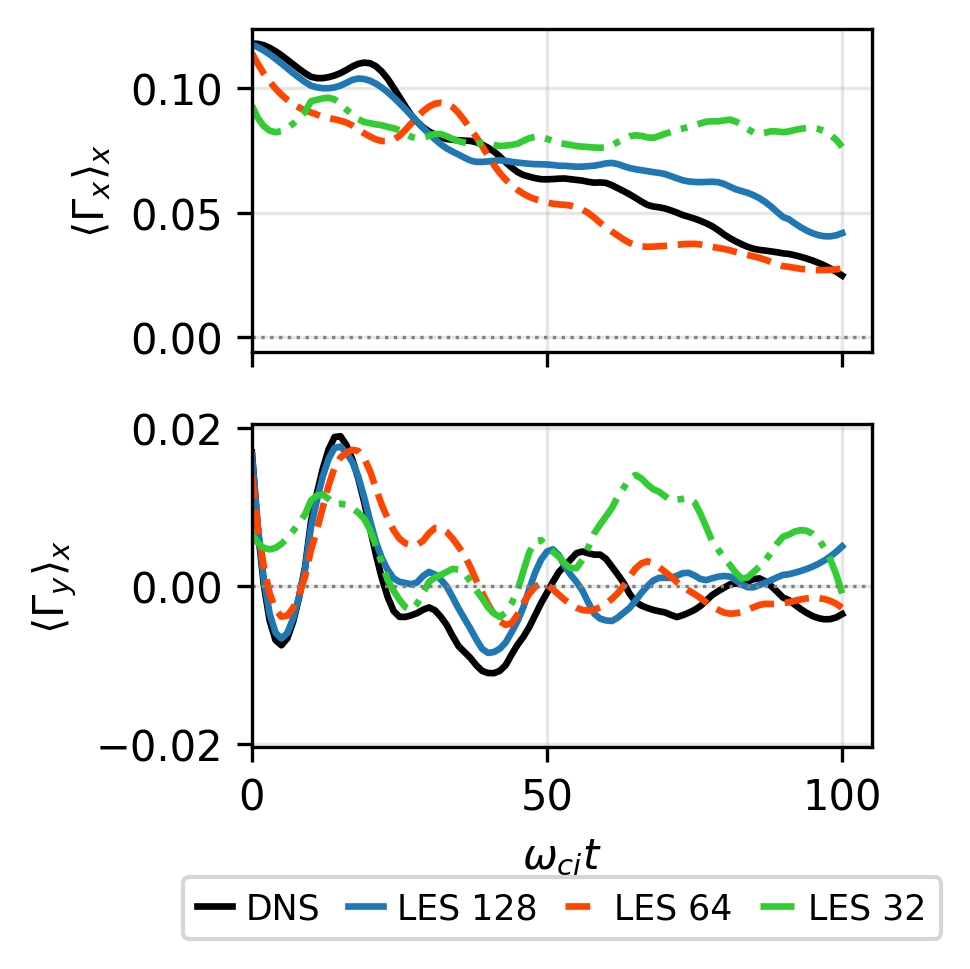
\includegraphics[width=\linewidth]{images/validation_current/mHW_N256/particle_flux_vs_time.png}
\caption{mHW\_N256}
\end{subfigure}
\hfill
\begin{subfigure}[t]{0.48\textwidth}
\centering
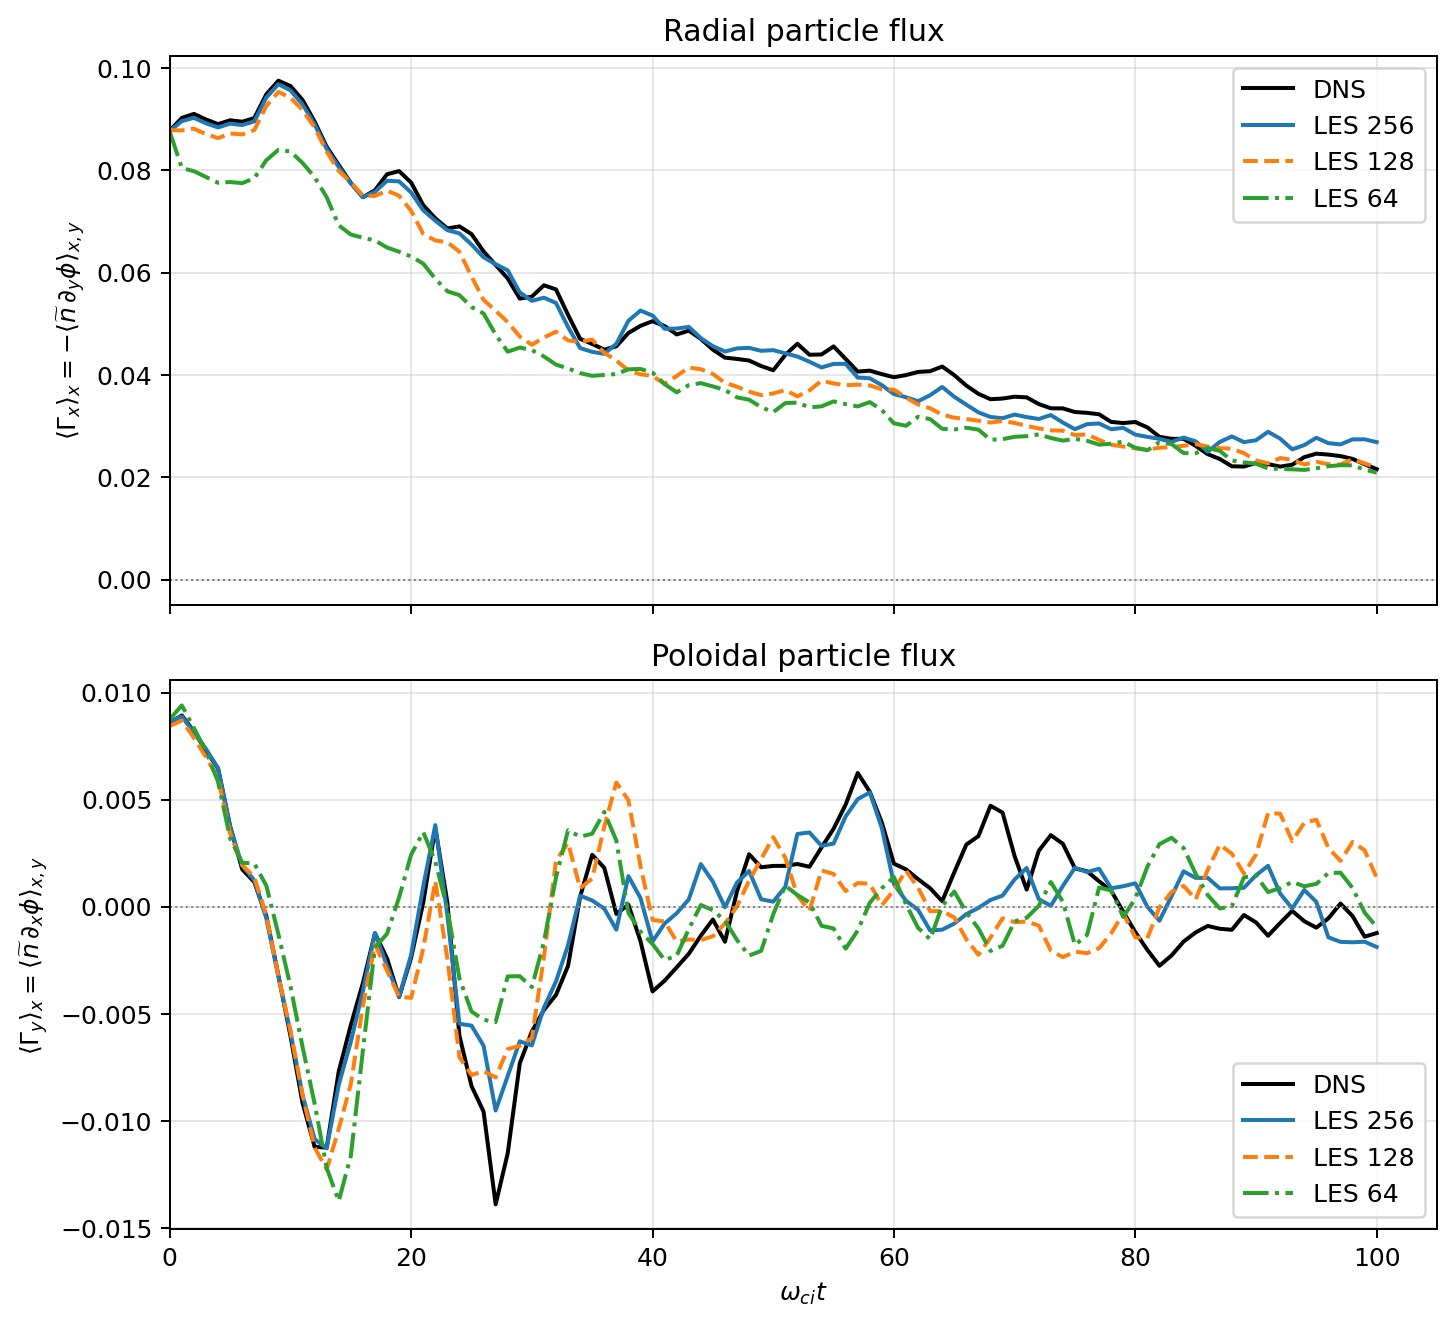
\includegraphics[width=\linewidth]{images/validation_current/mHW_N512/particle_flux_vs_time.png}
\caption{mHW\_N512}
\end{subfigure}
\caption{Domain-averaged radial (upper axes) and poloidal (lower axes) turbulent particle flux over $0\leq t\leq1000$ for HW and $0\leq t\leq100$ for mHW. Density fluctuations are defined relative to the poloidal mean. All three LES resolutions are shown for each available case.}
\label{fig:particle-flux}
\end{figure}

\subsection{Computational performance}

Wall-clock runtimes and MPI task counts were extracted from the final \texttt{Run time} entry and the \texttt{Processor number} entry, respectively, in the HW and mHW \texttt{BOUT.log.0} files. Each LES run is compared with the DNS run for the same model and reference resolution. The timing logs cover 1000 simulation time units for all 16 completed runs. These benchmark durations are distinct from the mHW statistical validation window, which is restricted to the first 100 time units. DNS uses 32 MPI tasks and LES uses one. Raw and duration-normalized wall-clock speedups therefore coincide. We define:
\begin{equation}
    S_{\mathrm{raw}}=\frac{T_{\mathrm{DNS}}}{T_{\mathrm{LES}}},
    \qquad
    S_{\mathrm{wall}}=
    \frac{T_{\mathrm{DNS}}/\Delta t_{\mathrm{DNS}}}
         {T_{\mathrm{LES}}/\Delta t_{\mathrm{LES}}},
    \qquad
    S_{\mathrm{MPI}}=S_{\mathrm{wall}}
    \frac{P_{\mathrm{DNS}}}{P_{\mathrm{LES}}},
\end{equation}
where $T$ is wall-clock runtime and $P$ is the number of MPI tasks. Here $S_{\mathrm{MPI}}$ measures the reduction in MPI task-time per unit simulated time; it is not a measured serial speedup. Values greater than unity indicate an improvement. Duration normalization compares average costs over the recorded trajectories rather than timings over an identical simulation interval.

\begin{table}[ht]
\centering
\small
\caption{Current HW and mHW runtimes extracted from \texttt{BOUT.log.0}. All runs cover 1000 simulation time units. Each DNS row is the baseline for its LES rows. Runtimes are displayed in minutes (m) and seconds (s), retaining the one-second precision reported by BOUT++; $S_{\mathrm{raw}}=S_{\mathrm{wall}}$ for these equal durations. For each case, we highlight the best performing $S_\mathrm{raw}$ and $S_\mathrm{wall}$ in bold.}
\label{tab:performance}
\begin{tabular}{lrrrr}
\toprule
Run & MPI tasks & Runtime & $S_{\mathrm{wall}}$ & $S_{\mathrm{MPI}}$ \\
\midrule
HW\_DNS256 & 32 & 4~m 36~s & \textbf{1.00} & 1.00 \\
HW\_DNS256\_LES32 & 1 & 7~m 19~s & 0.63 & \textbf{20.12} \\
HW\_DNS256\_LES64 & 1 & 12~m 42~s & 0.36 & 11.59 \\
HW\_DNS256\_LES128 & 1 & 27~m 26~s & 0.17 & 5.37 \\
\midrule
HW\_DNS512 & 32 & 59~m 3~s & 1.00 & 1.00 \\
HW\_DNS512\_LES64 & 1 & 42~m 25~s & \textbf{1.39} & \textbf{44.55} \\
HW\_DNS512\_LES128 & 1 & 92~m 5~s & 0.64 & 20.52 \\
HW\_DNS512\_LES256 & 1 & 320~m 41~s & 0.18 & 5.89 \\
\midrule
mHW\_DNS256 & 32 & 6~m 13~s & \textbf{1.00} & 1.00 \\
mHW\_DNS256\_LES32 & 1 & 21~m 27~s & 0.29 & 9.27 \\
mHW\_DNS256\_LES64 & 1 & 17~m 50~s & 0.35 & \textbf{11.16} \\
mHW\_DNS256\_LES128 & 1 & 41~m 17~s & 0.15 & 4.82 \\
\midrule
mHW\_DNS512 & 32 & 42~m 42~s & 1.00 & 1.00 \\
mHW\_DNS512\_LES64 & 1 & 27~m 38~s & \textbf{1.55} & \textbf{49.45} \\
mHW\_DNS512\_LES128 & 1 & 63~m 1~s & 0.68 & 21.68 \\
mHW\_DNS512\_LES256 & 1 & 185~m 37~s & 0.23 & 7.36 \\
\bottomrule
\end{tabular}
\end{table}

Table~\ref{tab:performance} shows MPI task-time reductions of 4.82--49.45 for the LES runs. The HW and mHW $512^2$ cases with $64^2$ LES meshes achieve wall-clock speedups of 1.39 and 1.55, respectively. All other LES runs have $S_{\mathrm{wall}}<1$. These measurements use integer-second runtimes and cover 1000 simulation time units per run. MPI task-time does not include accelerator resource costs, and these measurements do not quantify training cost or memory usage.


\section{Discussion}
The supplied results assess the evolution of reconstructed-field diagnostics; they do not compare against direct prediction of sub-grid terms. Physical consistency remains an important constraint on the reconstruction. In particular, calculating vorticity from the generated electrostatic potential enforces the elliptic relationship $\zeta=\nabla^2\phi$ and prevents independent-field drift.

The longer HW validation exposes a marked failure of the $32^2$ reconstruction for HW\_N256. For this case energy, generalized enstrophy and radial transport all collapse to levels well below DNS, and the endpoint PDFs become too narrow. Finer meshes retain more of the statistical behaviour, although instantaneous trajectories diverge. The mHW\_N512 results instead follow an early growth phase and subsequent decay through $t=100$, consistent with faster evolution toward laminarization. The different validation windows should therefore be interpreted in relation to the different dynamics, rather than as equal-duration stationary turbulence tests. The corrected mHW\_N256 diagnostics show that its $32^2$ reconstruction instead develops excess energy, enstrophy and radial transport, failing to reproduce the DNS decay. The two finer meshes retain the integral trends much more closely.

The approach has several limitations. First, the generator may produce nonphysical small-scale structures outside the training distribution. Second, long-time stability is not guaranteed solely by minimizing instantaneous reconstruction error. Finally, the present method is limited by the validity of the chosen filter and by the statistical coverage of the training dataset.
\todo[inline=true]{This last bit needs revised}
%----------------------------------------------------------------
%
%
%
%
%
%
%
%----------------------------------------------------------------
\section{Conclusions}\label{sec:Conclusions}

A hybrid AI-classical algorithm for edge-plasma LES closure has been developed by learning DNS fields filtered with a differential filter. We use the AI model to enhance the LES field towards a filtered DNS by removing details lost during the subsampling from DNS to LES resolutions. The DNS fields are then reconstructed by inverting the differential filter of \citet{germano_differential_1986}. The reconstructed fields are used to evaluate the nonlinear Poisson-bracket terms, while the vorticity is obtained directly from the generated electrostatic potential.

% The method was tested with the HW\_N256, HW\_N512, mHW\_N256 and mHW\_N512 configurations. The main conclusions are:

We benchmarked on the 2D Hasegawa-Wakatani and modified Hasegawa-Wakatani equations at two resolutions in BOUT++. Reconstructing from $32^2$ to $256^2$ resulted in poor prediction of the dynamics, as too much of the inertial subrange had been removed at this LES resolution, making the AI enhancement and differential filter inversion problematic. In all other cases, the time evolution statistics agreed well with the DNS for long time rollouts, showing enhanced stability compared to our previous study. This gave reasonable speedups of up to $1.5 \times$ on a single GPU (with LES on a single CPU), compared to DNS on 32 CPU cores. 
We expect larger speedups on larger problems such as 3D plasma turbulence, and parallelising the inference process for multi-CPU and multi-GPU. 
This will allow for accelerating edge plasma physics simulations for integration in powerplant design systems.

% \begin{itemize}
%     \item the generative model reconstructs the dominant spatial structures of the DNS fields;
%     \item the finer HW reconstructions retain several statistical features over 1000 time units, while the $32^2$ LES for HW\_N256 substantially underpredicts energy, enstrophy and radial transport;
%     \item the mHW\_N512 reconstruction captures the growth and subsequent decay through 100 time units; this shorter window reflects faster dynamics and the tendency toward laminarization;
%     \item the thousand-time-unit HW and mHW benchmarks show MPI task-time reductions of 4.82--49.45, with a maximum wall-clock speedup of 1.55 for mHW\_DNS512\_LES64;
%     \item the $32^2$ mHW\_N256 reconstruction develops excess energy, enstrophy and radial transport, whereas the finer meshes follow the DNS decay more closely; finite-window agreement does not establish stability beyond the tested conditions.
% \end{itemize}

% Future work will investigate parameter-conditioned generators, explicit enforcement of conservation laws, uncertainty quantification and extension to fully three-dimensional edge-plasma models such as Hermes-3.
%----------------------------------------------------------------
%
%
%
%
%
%
%
%----------------------------------------------------------------
\section*{Acknowledgements}

Simulations reported in this study were performed on X platform, funded by [TODO]. The authors acknowledge funding from X and UK-USA AI Partnership Programme (ISPF-240).

\bibliographystyle{elsarticle-harv}
\bibliography{references}


\end{document}
